% !TEX program = xelatex
% 使用 texlive 完整编译:
% xelatex -> bibtex -> xelatex -> xelatex
% zhbook 中文书籍 LaTeX 模板

%--- 正文前后都没有空白页 ---
% \documentclass[openany,twoside,zihao=-4]{zhbook}
% print 用于打印, 封面等生成空白页

%--- 正文前后都有空白页, 正文一章结束可空白页使新的一章是在奇数页开始 ---
\documentclass[twoside,openright,zihao=-4]{zhbook}


% 书籍信息设置
\title{线性代数之旁门左道}  % 标题
\subtitle{Linear Algebra Done Wrong}  % 副标题
\author{[美] Sergei Treil}  % 作者姓名
\date{\today}  % 日期
% \version{1.0}  % 版本
\bioinfo{译者}{吴俊达}  % 其他信息
\extrainfo{仅供个人学习使用，禁止商用}

% \extrainfo{\plogo \\[8pt] 出版社}

% 通用虚拟出版商标志
\newcommand{\plogo}{\fbox{$\mathcal{PL}$}}


%----- 设置英文字体 -----
% \usepackage{newtxtext}  %New TX font for text
\setmainfont{TeX Gyre Termes}  %Times New Roman 的开源复刻版本
% \setsansfont{TeX Gyre Termes}
% \setsansfont{TeX Gyre Heros}  %Helvetica 的开源复刻版本
% \setmonofont{TeX Gyre Cursor}  %Courier New 的开源复刻版本
% \setmainfont{Times New Roman}
% \setsansfont{Times New Roman}
\everydisplay{\def\arraystretch{0.8}}
\everymath{\def\arraystretch{0.8}}
%\setmonofont{Courier New}

%----- 设置数学字体 -----
%\usepackage{newtxmath}
%\usepackage{mathptmx}

%----- 添加其他宏包 -----
%\usepackage[notcite,notref]{showkeys}
\usepackage{listings}
% \usepackage{subfig}
\usepackage{nicematrix}
\usepackage{tikz}

%----- 取消链接颜色和方框 -----
%\hypersetup{hidelinks}

%----- 参考文献格式 -----
%\bibliographystyle{plain} % abbrv, unsrt, siam
\bibliographystyle{thuthesis-numeric}
%\bibliographystyle{thuthesis-author-year}

%----- 参考文献引用格式 -----
% \usepackage[numbers,sort&compress]{natbib}
%\usepackage[numbers,super,square,sort&compress]{natbib}
%\usepackage[authoryear,sort&compress]{natbib}
% \def\bibfont{\small}  % 修改参考文献字体
% \setlength{\bibsep}{7pt plus 3pt minus 3pt}  % 调整参考文献间距

%----- 制作索引 -----
% 自动编译 (默认字符编码排序)
%\usepackage{imakeidx}
%\makeindex[columns=2,intoc=true,title={索~~引}]
%\indexsetup{level=\chapter*}

% 可使用 zhmakeindex 改变索引排序 (默认拼音字母排序)
% \usepackage[noautomatic]{imakeidx}
\makeindex[columns=2,intoc=true,title={索~~引},options=xxx]


%----- 调整列表项的间距 -----
%\setlength{\itemsep}{3pt}

%----- 调整页面避免出现过大空白 -----
% \raggedbottom

%----- 定义符号描述命令  -----
\newcommand{\nameditem}[3][]{
\noindent\hspace{2em}\makebox[0.2\textwidth][l]{#2}{{#3}
\hfill\makebox[0.2\textwidth][l]{#1}\hspace*{2em}}\par}

%----- 插入 PDF 文件命令 -----
%\includepdf[pages=-]{pdfname.pdf}

%----- 微分算子 -----
\newcommand*{\dif}{\mathop{}\!\mathrm{d}}

%----- 自定义命令 -----
\newcommand{\CC}{\ensuremath{\mathbb{C}}}
\newcommand{\RR}{\ensuremath{\mathbb{R}}}
\newcommand{\A}{\mathcal{A}}
\newcommand{\tr}{\operatorname{trace}}
\newcommand{\nul}{\operatorname{Null}}
\renewcommand{\ker}{\operatorname{Ker}}
\newcommand{\rg}{\operatorname{Ran}}
\newcommand{\rank}{\operatorname{rank}}
\newcommand{\col}{\operatorname{Col}}
\newcommand{\ii}{\mathrm{i}\mkern1mu}
\newcommand{\abs}[1]{\lvert#1\rvert}
\newcommand{\norm}[1]{\left\lVert#1\right\rVert}
\newcommand{\dx}[1][x]{\mathop{}\!\mathrm{d}#1}
\newcommand{\red}[1]{\textcolor{red}{#1}}

\newCJKfontfamily\gothic{IPAexMincho}

%----- 脚注格式 -----
\usepackage{scrextend}
\renewcommand{\thefootnote}{[\arabic{footnote}]}
\deffootnote{2em}{1.5em}{\thefootnotemark\hspace{0.5em}}

\begin{document}


% 生成封面
\maketitle

% 插入封面 PDF文件
%\thispagestyle{empty}
%\includepdf{cover.pdf}
%\cleardoublepage


%%%%%%%%%%%%%%%%%%%%%%%%%%%%%%%%%%%%%%%%%%%%%%%%%%%

\frontmatter
%\pagenumbering{Roman} % 摘要页码为大写罗马数字

%%%%%%%%%%%%%%%%%%%%%% 前言 %%%%%%%%%%%%%%%%%%%%%%%%

\phantomsection
\chapter*{译者序}
\markboth{译者序}{译者序}
\addcontentsline{toc}{chapter}{译者序}
本书是对布朗大学Sergei Treil教授的著作《Linear Algebra Done Wrong》（更新于2024年10月1日）的翻译。
全书共分为9章，具体内容见后文“前言”一节，建议读者仔细阅读之，调整好阅读本书的心态和目标。

{\it 待完成：本书内容概要}

% 本书第一章引入一系列基本概念，首先是向量空间和线性组合，然后先引入基，再分别从存在性和唯一性引出张成和线性无关的概念。接下来介绍线性变换，借助矩阵的语言表述有关$\mathbb{F}^n$的情况，注重阐述了矩阵乘法的动机。然后介绍了可逆和同构。最后还给出了一小节应用实例。第二章。
% 第三章从低维几何角度（体积）引入行列式，同时也给出了基于置换的正式定义
% 本书对预备知识的要求低，语言通俗易懂，论述详细，
% 因此可作为非数学类学生的进阶自学用书，教师也可借此教材加开第二学期线性代数进阶课程。

% 特别感谢原书作者Sergei Treil教授及其同事的大力支持与热情鼓励。
本翻译使用的模板是在 \href{https://github.com/andy123t}{andy123t} 编写的 \href{https://github.com/andy123t/zhbook}{zhbook} 基础上修改而成的，
感谢 \href{https://github.com/andy123t}{andy123t} 精心打造这一美观的模板。

英文的表达习惯与中文有诸多不同，且原书语言生动，若直译难免生硬别扭、失其神韵。因此，
译者在充分尊重原文句意的前提下，对其中部分字眼不求字字对应，而根据自己的理解作了补充，必要时在脚注中作出解释。
翻译本质上是一种再创作，无法代替原著。希望读者不仅阅读翻译，更要能独立阅读原著，或者至少对照阅读一遍，
想必会更有收获。

由于译者只能利用业余时间进行翻译且水平有限，本翻译一定有不妥之处甚至错误，欢迎读者们多提意见和建议。
% 请将意见和建议发送至 \mailto{ladr2024@163.com}。

原书基于CC-BY-NC-ND 3.0许可协议发布，按照规定是不允许再创作的，此翻译版只是译者怀着帮助读者跨越“语言关”、更深入地掌握书中内容的朴素想法所作，译者不希望因此招致麻烦。所以，希望各位仅在课程群内交流，不要外传。谢谢大家。

{\hfill 译者\hspace{2em}}

{\hfill 2026年3月}

%%%%%%%%%%%%%%%%%%%% 前言 %%%%%%%%%%%%%%%%%%%%%

\begin{preface}

这本书的标题看上去有些故弄玄虚。如果这本书以“旁门左道”来讲线性代数，那人们为什么还要去读它呢？这本书的“旁”和“左”具体表现在哪里呢？

在回答这些问题之前，请允许我首先说明这本教材的目标读者群体。这本教材是“荣誉线性代数”课程的讲义。该课程是为数学基础较好的学生准备的{\bf 第一门}线性代数课程，面向虽还未熟悉抽象推理，但愿意超出“菜谱式”微积分课程而学习更加严谨的数学内容的学生，因而除作为线性代数入门课程外，本课程还旨在引导学生初步掌握{\bf 严谨}的数学证明与形式化定义——简言之，接触现代理论数学（抽象数学）的范式。目标读者要能借助通常在进阶教材中呈现的抽象定义和理论建构，来解释通常在入门线性代数教材中呈现的基本思想和具体实例。

本书另一特点是其编写视角并非来自代数专家，也非面向代数专家。因此我着重强调对分析学、几何学、概率论等领域重要的主题，省略了部分传统内容。例如，本书仅讨论实数域和复数域上的向量空间，完全不涉及其他域上的线性空间——因为我认为与其将时间用于介绍抽象域的概念，不如用来讲解其他学科需要掌握的经典主题。当学生后续在抽象代数课程中学习一般域的概念时，自会理解本书涉及的诸多理论结构同样适用于一般域。

此外，本书仅讨论有限维空间，且“基”均指有限基。原因在于：若不引入收敛性、范数、完备性等泛函分析基础概念，就无法对无限维空间进行深入讨论——而这显然是另一门课程（教材）的主题。因此本书不讨论无限哈默尔基：这类概念在分析和几何的大多数应用中并非必需，我认为它们更应属于抽象代数课程的范畴。

\subsection*{教学说明}

本书与通行的进阶线性代数教材存在若干差异。首先体现在基、线性无关性及生成组的定义方式上。我在书中首先将基定义为满足“任意向量都能唯一表示为线性组合”性质的向量组，随后基的两方面性质自然衍生出线性无关性（唯一性的体现）和生成性（存在性的体现）。

采用这种进路是因为，我认为基的概念远比线性无关性更重要——在大多数应用中，我们真正关心的是向量组能否构成基，而并不关注线性无关性。例如求解齐次方程组时，我们不仅需要线性无关解，更需要获取恰当数量的线性无关解（即解空间的基）。

并且，很容易向学生阐释基的重要性：基使我们能够引入坐标，从而可把研究抽象向量空间转化至研究$\mathbb{R}^n$（或$\mathbb{C}^n$）。此外，我们引入坐标是为了便于计算机运算——计算机尤其擅长矩阵处理。反观线性无关性的概念，我确实难以找到简明易懂的教学动机。

另一差异在于：我在讲解线性方程组解法之前先引入了线性变换。这种安排的缺点是直到第 \ref{chap:LinearSystems} 章才证明“仅方阵可逆”等重要结论。但是，提前定义线性变换能使行化简操作的阐述更具系统性。同时，我花费大量篇幅（两节）来阐释矩阵乘法的动机——希望充分说明这种看似奇特的乘法规则实则非常自然，且本质上是我们唯一的选择。

关于基、线性变换等的重要结论的证明（如向量空间中任意两个基包含相同数量向量这一结论）均在第 \ref{chap:LinearSystems} 章中，通过在行化简过程中数主元完成。尽管这些结论大多存在“无坐标”证明（形式上不涉及高斯消元法），但仔细分析便会发现：高斯消元与主元计数其实并未消失，只是暗含在多数证明过程中。因此，本书未采用进阶线性代数教材中常见的优雅却晦涩的“无坐标”证明，而是选用更常见于“微积分式”教材的“行化简”证明法——这样既能凸显诸证明背后的共同思路，也使数学基础有限的读者更易理解与记忆。

在第 \ref{chap:LinearSystems} 章第 \ref{sec:ChangeOfCoordinate} 节，我还提出了简单易记的基变换公式体系。

第 \ref{chap:Determinant} 章讨论行列式。我花费大量篇幅阐述行列式的来源，延后给出形式化定义。通过将行列式定义为体积计算工具，引导学生理解：若允许使用带符号体积以使行列式对各列是线性的（此时学生应已认识到线性的重要价值，且明白允许体积为负是其微不足道的代价）并假设若干自然性质，则必然推导出经典的行列式定义。需要强调的是，我并未先行设定行列式的反对称性，而是从体积的其他自然性质中推导得出。

需注意：虽然第 \ref{chap:BasicNotion} 至 \ref{chap:Determinant} 章形式上主要讨论实空间，但所有内容同样适用于复空间，甚至任意域上的向量空间。

第 \ref{chap:SpectralIntro} 章是谱理论入门，复空间$\mathbb{C}^n$在此自然登场（其形式定义虽在开篇已给出，但此前主要研究对象始终是实空间$\mathbb{R}^n$）。复特征值的出现表明：即便最初处理实矩阵（实空间上的算子），谱理论最自然的研究场域仍是复空间$\mathbb{C}^n$。本章重点在于对角化理论，并引入由特征空间构成的基的概念。

将涉及内积空间的第 \ref{chap:InnerProduct} 章置于谱理论之后，是因为我希望同步处理复数域与实数域情形，而谱理论为复空间提供了明确的动机。除却这层动机，第 \ref{chap:SpectralIntro}、\ref{chap:InnerProduct} 章内容相互独立，教师亦可选择先讲授第 \ref{chap:InnerProduct} 章。

尽管本书第 \ref{chap:SpectralAdvanced} 章介绍了若当标准形，但在单学期课程中通常没有时间涵盖该内容。我倾向于将更多时间用于第 \ref{chap:StructinInnerProdSpace}、\ref{chap:BilinearandInner} 章讨论的主题，例如正规算子与自伴算子的对角化、极分解与奇异值分解、正交矩阵的结构与取向，以及二次型理论。

我认为这些主题比若当标准形更具应用价值——尽管后者无疑具有理论美感。不过，我增设了第 \ref{chap:SpectralAdvanced} 章，因而教师能灵活调整教学内容：可选择跳过第 \ref{chap:StructinInnerProdSpace}、\ref{chap:BilinearandInner} 章部分主题，转而讲授若当分解定理。

本书（2009年版）还新增了关于对偶空间与张量的第 \ref{chap:DualandTensor} 章。我认为该部分内容（特别是张量相关章节）对一年级线性代数课程而言稍显拔高，但其中某些主题（如对偶空间中的坐标变换）可轻松纳入教学大纲。此外，该章也可作为进阶课程中张量理论的入门导引。需要说明的是，本章所有结论均适用于任意域。

在本书的呈现方式上，我力求采用非正式的表达风格：更倾向直观的几何推演而非形式化的代数运算，因此在纯粹主义者眼中本书可能不够严谨。全书通常将线性变换与其矩阵表示视为同一（只要不致引发混淆），这种简化标记法有助于初学者理解——过度强调变换及其矩阵的区别反而可能使初学者困惑。仅当这种区别至关重要时（例如分析基改变时线性变换矩阵的变化规律），我才会使用特殊标记法区分线性变换及其矩阵表示。

\end{preface}


% \phantomsection
\chapter*{翻译中更正的原书笔误}
\markboth{翻译中更正的原书笔误}{翻译中更正的原书笔误}

\section*{第6章}

{\bf 原书165页最后一行}：$\det(A-\lambda I)=(\lambda_1-\lambda)\det(A_1-\lambda)$应为$\det(A-\lambda I)=(\lambda_1-\lambda)\det(A_1-\lambda I)$

{\bf 原书197页习题6.4第一行}：$A=A^*>O$应为$A=A^*>0$

\section*{第7章}

{\bf 原书200页第2节第4段第4行}：$Q[{x}]=a_{1}x_{1}^{2}+a_{2}x_{2}^{2}+\ldots+a_{n}x_{n}^{2}$应为$Q[\mathbf{x}]=a_{1}x_{1}^{2}+a_{2}x_{2}^{2}+\ldots+a_{n}x_{n}^{2}$

{\bf 原书214页定理4.3证明第三段第一行}：$\mathbf{x}$应为$\mathbf{x}_0$

{\bf 原书216页最后一行}：$G=\{g_{j.k}\}_{j,k=1}^n$应为$G=\{g_{j,k}\}_{j,k=1}^n$

\section*{第9章}

{\bf 原书261页第三段}：$P(A)E\subset E$应为$p(A)E\subset E$

%%%%%%%%%%%%%%%%%%%%%%% 目录 %%%%%%%%%%%%%%%%%%%%%%%

% 生成目录
\maketoc

% 生成插图清单, 如不需要可以注释
% \makelof

% 生成表格清单, 如不需要可以注释
% \makelot

%%%%%%%%%%%%%%%%%%%% 主要符号表 %%%%%%%%%%%%%%%%%%%%%

% 如不需要可以注释
% \phantomsection
\chapter*{翻译版中更正的原书笔误}
\markboth{翻译版中更正的原书笔误}{翻译版中更正的原书笔误}

\section*{第1章}

{\bf 原书第6页（翻译第5页）定义2.1最后一段}：$x_{1}\mathbf{v}_{1}+x_{2}\mathbf{v}_{2}+\ldots+x_{m}\mathbf{v}_{n}=\mathbf{v}$改为$x_{1}\mathbf{v}_{1}+x_{2}\mathbf{v}_{2}+\ldots+x_{n}\mathbf{v}_{n}=\mathbf{v}$

{\bf 原书第6页例2.2最后一个行间公式（翻译第6页）}：$\mathbf{v}=x_1\mathbf{e}_1+x_2\mathbf{e}_2+\ldots x_n\mathbf{e}_n=\sum_{k=1}^nx_k\mathbf{e}_k$改为$\mathbf{v}=x_1\mathbf{e}_1+x_2\mathbf{e}_2+\ldots +x_n\mathbf{e}_n=\sum_{k=1}^nx_k\mathbf{e}_k$

{\bf 原书第8页线性组合定义的第一段（翻译第8页）}：$\alpha_{k}=\mathbf{0}\ \forall k$改为$\alpha_{k}=0\ \forall k$

{\bf 原书第12页（翻译第11页）“反射”的例子}：see the fig（见图）应该在上面的例子中。

{\bf 原书第20页第一个行间公式（翻译第19页）}：$\forall {x}\in\mathbb{F}^r$应为$\forall \mathbf{x}\in\mathbb{F}^r$

{\bf 原书第28页第3点（翻译第26页）}：is isomorphic to $\mathbb{R}^6$应为is isomorphic to $\mathbb{F}^6$

{\bf 原书第36页脚注3（翻译第33页）}：$\mathbb{R}^2$应为$\mathbb{R}^3$，$0$应为$\mathbf{0}$

\section*{第3章}

{\bf 原书79页第一个行间公式}：第一行多了一个等号


%%%%%%%%%%%%%%%%%%%%%%%%%%%%%%%%%%%%%%%%%%%%%%%%%%%%

\mainmatter

%%%%%%%%%%%%%%%%%%%% 正文内容 %%%%%%%%%%%%%%%%%%%%%%%


%----- 第1章 基本概念 -----

%%%%%%%%%%%%%%%%%%%% 基本概念 %%%%%%%%%%%%%%%%%%%%%

\chapter{基本概念}\label{chap:BasicNotion}

\section{向量空间}\label{sec:vector_space}

向量空间$V$是一系列对象所构成的（非空）集合，这些对象称为向量（本书中以粗体小写字母表示，例如$\mathbf{v}$）。其上还定义了两种运算——向量的加法以及向量与数（标量）的乘法\footnote{我们需要让向量和其他对象看起来有些区别，因此在本书中我们使用粗体小写字母来表示向量，并用正体小写字母来表示数（标量）。一些（进阶的）教材中，拉丁字母用于表示向量而希腊字母用于表示标量；更为进阶的教材里，任意字母可用于表示任意对象，而读者须从上下文推断每个符号的含义。我认为，尤其对于初学者而言，对不同对象加以视觉上的区分是有助于理解的，因此总用粗体小写字母来表示向量。在黑板上，则用箭头来标识向量（如$\vec{v}$所示）。}，这两种运算满足所得结果总属于$V$，以及以下的八条性质（所谓向量空间的{\bf 公理}）：

前 4 条性质是关于加法的：\marginpar{\small 问题来了：“这些性质怎么记得住呢？”回答是，并不需要记忆，详见后文！}
\begin{enumerate}
    \item 交换律：对于所有 $\mathbf{v},\mathbf{w}\in V$，都有$\mathbf{v} + \mathbf{w} = \mathbf{w} + \mathbf{v}$；
    \item 结合律：对于所有 $\mathbf{u},\mathbf{v},\mathbf{w}\in V$，都有$(\mathbf{u}+\mathbf{v})+\mathbf{w}=\mathbf{u}+(\mathbf{v}+\mathbf{w})$；
    \item 零向量：存在一个特殊的向量，记作$\mathbf{0}$，其满足$\mathbf{v}+\mathbf{0} = \mathbf{v}$对于所有$\mathbf{v}\in V$都成立；
    \item 加法逆元：对于每个向量$\mathbf{v}\in V$，都存在向量$\mathbf{w}\in V$使得$\mathbf{v}+\mathbf{w}=\mathbf{0}$。这一加法逆元常记作$-\mathbf{v}$；
\end{enumerate}

接下来两条性质是有关乘法的：

\begin{enumerate}[start=5]
    \item 乘法恒等元：对于所有$\mathbf{v}\in V$，都有$1\mathbf{v}=\mathbf{v}$；
    \item 乘法结合律：对于所有$\mathbf{v}\in V$和所有标量$\alpha,\beta$，都有$(\alpha\beta)\mathbf{v} = \alpha(\beta\mathbf{v})$；
\end{enumerate}

最后是两条分配性质，它们将乘法与加法联系起来：

\begin{enumerate}[start=7]
    \item 对于所有$\mathbf{u},\mathbf{v}\in V$和所有标量$\alpha$，都有$\alpha(\mathbf{u}+\mathbf{v})=\alpha\mathbf{u}+\alpha\mathbf{v}$；
    \item 对于所有$\mathbf{v}\in V$和所有标量$\alpha,\beta$，都有$(\alpha+\beta)\mathbf{v}=\alpha\mathbf{v}+\beta\mathbf{v}$。
\end{enumerate}

\begin{remark*}
    上述性质看起来很难记忆，但其实没必要记——它们就是标量代数的运算律，而这些内容你在中学期间就已经知道了。唯一新出现的难点是，你需要理解运算可作用的对象。你可以将向量相加，也可以将向量与数（标量）相乘。当然，你还可以对于数进行之前你学过的所有运算。然而，你不能将两个向量相乘，或将向量和数加在一起。
\end{remark*}

\begin{remark*}
    容易证明，零向量$\mathbf{0}$是唯一的，并且对于给定$\mathbf{v}\in V$，其加法逆元$-\mathbf{v}$也是唯一的。

    同样，（利用性质5、6和8）不难证明$\mathbf{0} = 0\mathbf{v}$对所有$\mathbf{v}\in V$都成立，且有$-\mathbf{v}=(-1)\mathbf{v}$。注意，在证明过程中，我们还需用到向量空间的其他性质，特别是性质3和4。
\end{remark*}

若标量为实数，那么我们称$V$为{\bf 实}向量空间。若标量为复数，意即我们可将向量与复数相乘，那么我们称$V$为{\bf 复}向量空间。

注意，任何的复向量空间也是实向量空间（如果我们可以做复数乘法，那么也可以做实数乘法），但反之不成立。

还可以考虑标量为任意的域$\mathbb{F}$中的元素的情况。\marginpar{\small 如果你不知道什么是域也不必担心，因为在这本书中我们只考虑实向量空间和复向量空间。}在这种情况里，我们说$V$是域$\mathbb{F}$上的向量空间。尽管本书的许多章节（特别地，第 \ref{chap:BasicNotion} 至 \ref{chap:Determinant} 章的全部内容）对于一般的域都适用，在本书中我们只考虑实向量空间和复向量空间。

如果我们不指明标量集合或使用$\mathbb{F}$来指代之，那么有关结论就对实向量空间和复向量空间都成立。如果需要区分实向量空间和复向量空间，那么我们就会说清楚到底在考虑何种情况。

注意，在“任意的域上的向量空间”这一定义中，我们{\bf 要求}标量集合为域，这样我们总是可以与非零标量做除法（并且不产生余数）。于是，向量空间的标量集可以取为有理数集，但不能取为整数集。

\subsection{例子}
\begin{example*}
    向量空间$\mathbb{R}^n$由长度为$n$的列向量（如下）所构成：
    \[\mathbf{v}=\begin{pmatrix}v_1\\v_2\\\vdots\\v_n\end{pmatrix}\]
    其中各项为实数。加法和乘法是逐项定义的，也即
    \[\alpha\begin{pmatrix}v_1\\v_2\\\vdots\\v_n\end{pmatrix}=\begin{pmatrix}\alpha v_1\\\alpha v_2\\\vdots\\\alpha v_n\end{pmatrix},\quad\begin{pmatrix}v_1\\v_2\\\vdots\\v_n\end{pmatrix}+\begin{pmatrix}w_1\\w_2\\\vdots\\w_n\end{pmatrix}=\begin{pmatrix}v_1+w_1\\v_2+w_2\\\vdots\\v_n+w_n\end{pmatrix}\]
\end{example*}

\begin{example*}
    向量空间$\mathbb{C}^n$同样由长度为$n$的列向量所构成，只是向量中各项为复数。加法和乘法与$\mathbb{R}^n$中的定义相同，唯一的区别在于如今可以将向量与{\bf 复}数相乘，也即，$\mathbb{C}^n$为{\bf 复}向量空间。
\end{example*}

本书中许多结论对于$\mathbb{R}^n$和$\mathbb{C}^n$都成立，在这样的情况下，我们将使用$\mathbb{F}^n$这个记号。

\begin{example*}
    向量空间$M_{m\times n}$（也记作$M_{m,n}$）由$m\times n$矩阵构成，加法和标量乘法是逐项定义的。如果我们限制各项为实数（并且只允许与实数相乘），那么我们就得到了一个实向量空间；如果我们允许各项为复数（并且允许与复数相乘），那么我们就得到了一个复向量空间。

    正式而言，我们需要区分实数与复数情形，也即分别写为$M_{m, n}^{\mathbb{R}}$和$M_{m, n}^{\mathbb{C}}$。然而，在大多数场合中，实数和复数情形并没有区别，于是也没有必要明确到底在考虑哪种情形。如果有所区别，我们会说清楚考虑的是哪种情况。
\end{example*}

\begin{remark*}
    如上所提到的，向量空间的公理仅仅是实数或复数的通常代数运算规则，因此如果我们将标量（数）视作向量，那么所有的公理都是成立的。于是，实数集合$\mathbb{R}$是实向量空间，复数集合$\mathbb{C}$是复向量空间。

    更重要的是，由于在上面的例子中，所有的向量运算（加法和标量乘法）都是逐项进行的，因此在这些例子中向量空间的公理是自动满足的，因为这些公理对标量成立（你能看出原因吗？）。因此，无需检验这些公理，我们就能得知上述例子中的集合的确是向量空间！

    同样的道理也适用于下面的例子，此处多项式的系数充当了（上述列向量或矩阵中）各项的角色。
\end{remark*}

\begin{example*}
    由次数至多为$n$的多项式所构成的向量空间$\mathbb{P}_n$，其中各元素$p$都是多项式，形式如下：\[p(t) = a_0 + a_1t + a_2t^2 + \dots +a_nt^n,\]
    其中$t$为自变量。注意，有些（甚至全部）系数$a_k$可以取$0$。

    系数$a_k$为实数时，我们就得到了一个实向量空间；系数$a_k$为复数时，此空间则为复向量空间。同样，仅在有必要的时候我们才说明考虑的是实数情形还是复数情形，否则所讨论的内容在两种情况下都适用。
\end{example*}

{\bf 问题：}上面这几个例子中的零向量是什么？

\subsection{矩阵记号}\label{subsec:matrix_notation}

一个$m\times n$的矩阵是一个有$m$行$n$列的数阵。这个阵列中的元素称为矩阵的{\bf 项}。

将矩阵的项记作带下标的字母是很方便的：第一个下标代表该项的行号，而第二个下标则代表列号。例如
\begin{equation}\label{matrix_notation}
    A=(a_{j,k})_{j=1,k=1}^{m,\quad n}=\begin{pmatrix}a_{1,1}&a_{1,2}&\ldots&a_{1,n}\\a_{2,1}&a_{2,2}&\ldots&a_{2,n}\\\vdots&\vdots&&\vdots\\a_{m,1}&a_{m,2}&\ldots&a_{m,n}\end{pmatrix}
\end{equation}
就是$m\times n$矩阵的通常表示形式。

矩阵$A$中的第$j$行第$k$列的项往往表示为$A_{j,k}$或$(A)_{j,k}$，有时也像上面的式 \eqref{matrix_notation} 那样用小写字母加下标来表示。

给定一矩阵$A$，其{\bf 转置}（或转置矩阵）$A^T$定义为将$A$的行变为列所得的矩阵。例如
\[\begin{pmatrix}1&2&3\\4&5&6\end{pmatrix}^T=\begin{pmatrix}1&4\\2&5\\3&6\end{pmatrix}.\]
因此，$A^T$的各列就是$A$的各行。反之亦然：$A^T$的各行就是$A$的各列。

正式的定义是：$(A^T)_{j,k}=(A)_{k,j}$，意为：$A^T$的第$j$行第$k$列的项等于$A$的第$k$行第$j$列的项。

就线性变换而言，矩阵的转置可用于给出一个很优美的阐释，也即其能导出所谓{\bf 伴随}变换，我们将在后面详细研究它，目前转置仅仅是一种有用且正式的运算。

转置的用处首先在于使我们得以将列向量$\mathbf{x}\in\mathbb{F}^n$（回想一下，$\mathbb{F}$是指$\mathbb{R}$或$\mathbb{C}$）写为$\mathbf{x} = (x_1,x_2,\dots,x_n)^T$。如果我们将列向量竖着写，那么其占据的空间就会大大增加。

\begin{problemset}
\item 令$\mathbf{x}=(1,2,3)^{T},\mathbf{y}=(y_{1},y_{2},y_{3})^{T},\mathbf{z}=(4,2,1)^{T}$。计算$2\mathbf{x},3\mathbf{y},\mathbf{x}+2\mathbf{y}-3\mathbf{z}$。
\item 下面哪些集合（具有自然的加法和标量乘法运算）是向量空间？论证你的结论。
\begin{probenumerate}
    \item 所有区间$[0,1]$上的连续函数所成的集合；
    \item 所有区间$[0,1]$上的非负函数所成的集合；
    \item 所有次数{\bf 恰}为$n$的多项式所成的集合；
    \item 所有$n\times n$对称矩阵所成的集合，即所有满足$A^T=A$的矩阵$A=\{a_{j,k}\}_{j,k=1}^n$所成的集合。
\end{probenumerate}
\item 判断正误：
\begin{probenumerate}
    \item 每个向量空间都包含零向量；
    \item 一向量空间可包含多个零向量；
    \item $m\times n$矩阵有$m$行$n$列；
    \item 若$f$和$g$是次数为$n$的多项式，那么$f+g$也是次数为$n$的多项式；
    \item 若$f$和$g$是次数至多为$n$的多项式，那么$f+g$也是次数至多为$n$的多项式。
\end{probenumerate}
\item 证明：向量空间$V$的零向量$\mathbf{0}$唯一。
\item 向量空间$M_{2\times 3}$的零向量是何矩阵？
\item 证明：向量空间公理4所定义的加法逆元是唯一的。
\item 证明：$0\mathbf{v} = \mathbf{0}$对于所有向量$\mathbf{v}\in V$都成立。
\item 证明：对于所有向量$\mathbf{v}$，其加法逆元$-\mathbf{v}$由$(-1)\mathbf{v}$给出。
\end{problemset}

\section{线性组合、基}

令$V$为一向量空间，并令$\mathbf{v}_{1},\mathbf{v}_{2},\ldots,\mathbf{v}_{p}\in V$为一系列向量。向量$\mathbf{v}_{1},\mathbf{v}_{2},\ldots,\mathbf{v}_{p}$的{\bf 线性组合}是形式如下的求和式：
\[\alpha_1\mathbf{v}_1+\alpha_2\mathbf{v}_2+\ldots+\alpha_p\mathbf{v}_p=\sum_{k=1}^p\alpha_k\mathbf{v}_k.\]

\begin{definition}
    称一组向量\footnote{原书对于若干向量有两种表达：“a system of vectors”和“a set of vectors”，此处一律采用国内通行翻译“向量组”。——译者注}$\mathbf{v}_{1},\mathbf{v}_{2},\ldots,\mathbf{v}_{n}\in V$为（向量空间$V$的）基，若任意向量$\mathbf{v}\in V$都能被{\bf 唯一}写成线性组合的形式：\[\mathbf{v}=\alpha_1\mathbf{v}_1+\alpha_2\mathbf{v}_2+\ldots+\alpha_n\mathbf{v}_n=\sum_{k=1}^n\alpha_k\mathbf{v}_k.\]
    系数$\alpha_1,\alpha_2,\dots,\alpha_n$称为向量$\mathbf{v}$（在基下，或者说关于基$\mathbf{v}_{1},\mathbf{v}_{2},\ldots,\mathbf{v}_{n}$）的{\bf 坐标}。

    $\mathbf{v}_{1},\mathbf{v}_{2},\ldots,\mathbf{v}_{n}$是基的另一种表述是，方程$x_{1}\mathbf{v}_{1}+x_{2}\mathbf{v}_{2}+\ldots+x_{n}\mathbf{v}_{n}=\mathbf{v}$（未知数为各$x_k$）对于任意右端项$\mathbf{v}$皆有唯一解。
\end{definition}

在讨论基的性质之前，首先给出一些例子来说明“基”这种对象确实存在，并且研究它们是有意义的。

\begin{example}
    在这第一个例子当中，向量空间$V$等于$\mathbb{F}^n$，其中$\mathbb{F}$是$\mathbb{R}$或$\mathbb{C}$。考虑向量
    \[\mathbf{e}_1=\begin{pmatrix}1\\0\\0\\\vdots\\0\end{pmatrix},\quad\mathbf{e}_2=\begin{pmatrix}0\\1\\0\\\vdots\\0\end{pmatrix},\quad\mathbf{e}_3=\begin{pmatrix}0\\0\\1\\\vdots\\0\end{pmatrix},\ldots,\quad\mathbf{e}_n=\begin{pmatrix}0\\0\\0\\\vdots\\1\end{pmatrix},\]
    （向量$\mathbf{e}_k$除第$k$项为$1$外，其余各项均为$0$）。
    
    向量组$\mathbf{e}_1,\mathbf{e}_2,\dots,\mathbf{e}_n$是$\mathbb{F}^n$的基。的确，任意向量\[\mathbf{v}=\begin{pmatrix}x_1\\x_2\\\vdots\\x_n\end{pmatrix}\in\mathbb{F}^n\]
    都能被表示成线性组合
    \[\mathbf{v}=x_1\mathbf{e}_1+x_2\mathbf{e}_2+\ldots +x_n\mathbf{e}_n=\sum_{k=1}^nx_k\mathbf{e}_k\]
    且该表示唯一。向量组$\mathbf{e}_1,\mathbf{e}_2,\dots,\mathbf{e}_n$称为$\mathbb{F}^n$的{\bf 标准基}。
\end{example}

\begin{example}
    本例中考虑的是次数至多为$n$的多项式所构成的向量空间$\mathbb{P}_n$。考虑定义如下的向量（多项式）$\mathbf{e}_0,\mathbf{e}_1,\mathbf{e}_2,\dots,\mathbf{e}_n\in \mathbb{P}_n$
    \[\mathbf{e}_0:=1,\quad\mathbf{e}_1:=t,\quad\mathbf{e}_2:=t^2,\quad\mathbf{e}_3:=t^3,\quad\ldots,\quad\mathbf{e}_n:=t^n.\]
    显然，对任意多项式$p$，$p(t)=a_0+a_1t+a_2t^2+\ldots+a_nt^n$，其均能被唯一表示为
    \[p=a_0\mathbf{e}_0+a_1\mathbf{e}_1+\ldots+a_n\mathbf{e}_n.\]
    因此向量组$\mathbf{e}_0,\mathbf{e}_1,\mathbf{e}_2,\ldots,\mathbf{e}_n\in\mathbb{P}_n$是$\mathbb{P}_n$的基。我们称其为$\mathbb{P}_n$的标准基。
\end{example}

\begin{remark}\label{remark:fn_to_abstract}
    若向量空间$V$有基$\mathbf{v}_{1},\mathbf{v}_{2},\ldots,\mathbf{v}_{n}$，\marginpar{\small 这个注记很重要，整本书都会用到它。它使我们得以将适用于标准向量空间$\mathbb{F}^n$的各种表述迁移至具有基$\mathbf{v}_{1},\mathbf{v}_{2},\ldots,\mathbf{v}_{n}$的向量空间$V$。}那么任意向量$\mathbf{v}$都能被线性组合式$\mathbf{v}=\sum_{k=1}^{n}\alpha_{k}\mathbf{v}_{k}$中的系数唯一决定。因此，如果我们将各系数$\alpha_k$写在一列中，那么我们处理任意向量就如同处理列向量一样，也就是如同处理$\mathbb{F}^n$中的元素一样（此处$\mathbb{F}$仍然代表$\mathbb{R}$或$\mathbb{C}$，不过此处的结论对于任意的域$\mathbb{F}$也是成立的）。

    这就是说，若$\mathbf{v}=\sum_{k=1}^{n}\alpha_{k}\mathbf{v}_{k}$且$\mathbf{w}=\sum_{k=1}^{n}\beta_{k}\mathbf{v}_{k}$，则
    \[\mathbf{v}+\mathbf{w}=\sum_{k=1}^n\alpha_k\mathbf{v}_k+\sum_{k=1}^n\beta_k\mathbf{v}_k=\sum_{k=1}^n(\alpha_k+\beta_k)\mathbf{v}_k,\]
    即为了得到求和结果的坐标所构成的列向量，只需将各求和项的坐标所构成的列向量相加。类似地，为了得到$\alpha\mathbf{v}$的坐标，我们只需将$\mathbf{v}$的坐标所构成的列向量乘以$\alpha$。
\end{remark}

\subsection{生成组与线性无关组}

基的定义中说到，任意向量都能被唯一表示成基向量的线性组合。这个说法其实包含两方面：一是表达式存在，二是表达式唯一。让我们分开来分析这两个方面。

如果我们只考虑存在性，我们就得到下面的概念：

\begin{definition}
    称一组向量$\mathbf{v}_{1},\mathbf{v}_{2},\ldots,\mathbf{v}_{p}\in V$为$V$中的生成组（也称为{\bf 张成组}或{\bf 完备组}），若任意向量$\mathbf{v}\in V$都能被写成线性组合的形式：\[\mathbf{v}=\alpha_1\mathbf{v}_1+\alpha_2\mathbf{v}_2+\ldots+\alpha_p\mathbf{v}_p=\sum_{k=1}^p\alpha_k\mathbf{v}_k.\]
\end{definition}

该定义与基的定义的唯一区别在于，我们并不假设上述表示形式唯一。

此处{\bf 生成}、{\bf 张成}和{\bf 完备}是同义词。我本人更喜欢“完备”这个词，这是由于我在算子理论方面的专业背景。“生成”和“张成”则更经常用于线性代数教材中。

显然，任一基都是张成（完备）向量组。并且，如果我们向基$\mathbf{v}_{1},$ $\mathbf{v}_{2},\ldots,\mathbf{v}_{n}$中加入若干向量$\mathbf{v}_{n+1},\ldots,\mathbf{v}_{p}$，那么新的向量组是张成（完备）向量组。的确如此：我们可以将任意向量表示成$\mathbf{v}_{1},\mathbf{v}_{2},\ldots,$ $\mathbf{v}_{n}$的线性组合，并直接忽略新加入的向量（取对应的系数$\alpha_k=0$）。

现在，让我们将注意力转向唯一性。我们不想产生存在性方面的顾虑，因此我们考虑零向量$\mathbf{0}$，其总是能够以线性组合式表出。

\begin{definition*}
    称线性组合$\alpha_{1}\mathbf{v}_{1}+\alpha_{2}\mathbf{v}_{2}+\ldots+\alpha_{p}\mathbf{v}_{p}$是{\bf 平凡的}，若$\alpha_k = 0\ \forall k$。
\end{definition*}

平凡的线性组合总等于$\mathbf{0}$（无论向量$\mathbf{v}_1,\mathbf{v}_2,\ldots,\mathbf{v}_p$是什么），这可能也是其名称的来历。

\begin{definition*}
    称一组向量$\mathbf{v}_{1},\mathbf{v}_{2},\ldots,\mathbf{v}_{p}\in V$为{\bf 线性无关的}，若$\mathbf{v}_{1},\mathbf{v}_{2},\ldots,\mathbf{v}_{p}$只有平凡线性组合（$\sum_{k=1}^{p}\alpha_{k}\mathbf{v}_{k}$，其中$\alpha_{k}=0\ \forall k$）等于$\mathbf{0}$。

    换言之，向量组$\mathbf{v}_{1},\mathbf{v}_{2},\ldots,\mathbf{v}_{p}$是线性无关的，当且仅当方程$x_1\mathbf{v}_1+x_2\mathbf{v}_2+\ldots+x_p\mathbf{v}_p=\mathbf{0}$（未知数为$x_k$）仅有平凡解（$x_{1}=x_{2}=\ldots=x_{p}=0$）。
\end{definition*}

若一向量组不是线性无关的，就称其为{\bf 线性相关的}。通过取线性无关定义的否定，我们得到以下定义：

\begin{definition*}
    称一组向量$\mathbf{v}_{1},\mathbf{v}_{2},\ldots,\mathbf{v}_{p}\in V$为{\bf 线性相关的}，若$\mathbf{0}$可被表示为非平凡的线性组合$\mathbf{0}=\sum_{k=1}^{p}\alpha_{k}\mathbf{v}_{k}$。此处的“非平凡”是指至少一个系数$\alpha_{k}$是非零的。这可以写为（也通常表示为）$\sum_{k=1}^{p}|\alpha_{k}|\neq0$。
\end{definition*}

换种方式表述该定义，我们可以说，向量组$\mathbf{v}_{1},\mathbf{v}_{2},\ldots,\mathbf{v}_{p}$是线性相关的，当且仅当存在标量$\alpha_1,\alpha_2,\ldots,\alpha_p$且$\sum_{k=1}^{p}|\alpha_{k}|\neq0$使得\[\sum_{k=1}^p\alpha_k\mathbf{v}_k=\mathbf{0}.\]

还有一种定义（以方程的语言表述）是：向量组$\mathbf{v}_{1},\mathbf{v}_{2},\ldots,\mathbf{v}_{p}$是线性相关的，当且仅当方程\[x_1\mathbf{v}_1+x_2\mathbf{v}_2+\ldots+x_p\mathbf{v}_p=\mathbf{0}\]
（未知数为$x_k$）有非平凡解。此处的“非平凡”还是指至少一个$x_{k}$是非零的，并可写作$\sum_{k=1}^{p}|x_{k}|\neq0$。

以下命题又给出了线性相关组的一种描述。
\begin{proposition}
    一组向量$\mathbf{v}_{1},\mathbf{v}_{2},\ldots,\mathbf{v}_{p}\in V$是线性相关的，当且仅当其中有一向量$\mathbf{v}_{k}$可被表示成其他向量的线性组合
    \begin{equation}\label{eq_2_1}
        \mathbf{v}_k=\sum_{\begin{subarray}{c}j=1\\j\neq k\end{subarray}}^p\beta_j\mathbf{v}_j.
    \end{equation}
\end{proposition}
\begin{proof}
    假设向量组$\mathbf{v}_{1},\mathbf{v}_{2},\ldots,\mathbf{v}_{p}$是线性相关的。那么存在标量$\alpha_{k}$，\\$\sum_{k=1}^{p}|\alpha_{k}|\neq0$使得
    \[\alpha_1\mathbf{v}_1+\alpha_2\mathbf{v}_2+\cdots+\alpha_p\mathbf{v}_p=\mathbf{0}.\]
    令$k$为使得$\alpha_k\ne 0$的下标。于是，将除了$\alpha_{k}\mathbf{v}_{k}$之外的项移到右端可得\[\alpha_k\mathbf{v}_k=-\sum_{\begin{subarray}{c}j=1\\j\neq k\end{subarray}}^p\alpha_j\mathbf{v}_j.\]
    将两边都除以$\alpha_k$可得式 \eqref{eq_2_1}，其中$\beta_j = -\alpha_j/\alpha_k$。

    另一方面，若 \eqref{eq_2_1} 成立，那么$\mathbf{0}$可被表示为非平凡线性组合\[\mathbf{v}_k-\sum_{\begin{subarray}{c}j=1\\j\neq k\end{subarray}}^p\beta_j\mathbf{v}_j=\mathbf{0}.\]
\end{proof}

显然，任一基都是线性无关组。的确如此：若向量组$\mathbf{v}_{1},\mathbf{v}_{2},\ldots,\mathbf{v}_{n}$是基，那么$\mathbf{0}$可被唯一表示为\[\mathbf{0}=\alpha_1\mathbf{v}_1+\alpha_2\mathbf{v}_2+\cdots+\alpha_n\mathbf{v}_n=\sum_{k=1}^n\alpha_k\mathbf{v}_k.\]
由于$\mathbf{0}$总可被平凡线性组合表出，所以平凡线性组合就是{\bf 唯一}线性表出$\mathbf{0}$的方法。

\marginpar{\small 在许多教材中，基被定义为既完备又线性无关的向量组。由命题 \ref{prop:complete_li_basis}，这种定义和本书的定义是等价的。}

所以，如我们已经讨论的，若一向量组是基，则其是完备（生成）组，也是线性无关组。下面命题表明，这句话反过来也是成立的。

\begin{proposition}\label{prop:complete_li_basis}
    向量组$\mathbf{v}_{1},\mathbf{v}_{2},\ldots,\mathbf{v}_{n}\in V$是基，当且仅当其既是完备（生成）组又线性无关。
\end{proposition}

\begin{proof}
    我们已经知道基一定是既完备又线性无关的，所以该命题的一个方向已经得证了。

    让我们证明另一个方向。设向量组$\mathbf{v}_{1},\mathbf{v}_{2},\ldots,\mathbf{v}_{n}$是线性无关且完备的。取任意向量$\mathbf{v}\in V$。因为向量组$\mathbf{v}_{1},\mathbf{v}_{2},\ldots,\mathbf{v}_{n}$是完备（生成）组，因此$\mathbf{v}$可表示为\[\mathbf{v}=\alpha_1\mathbf{v}_1+\alpha_2\mathbf{v}_2+\cdots+\alpha_n\mathbf{v}_n=\sum_{k=1}^n\alpha_k\mathbf{v}_k.\]
    我们只需证明此表达式是唯一的。

    设$\mathbf{v}$还可被表示为\[\mathbf{v}=\sum_{k=1}^{n}\widetilde{\alpha}_{k}\mathbf{v}_{k}.\]
    那么\[\sum_{k=1}^n(\alpha_k-\widetilde{\alpha}_k)\mathbf{v}_k=\sum_{k=1}^n\alpha_k\mathbf{v}_k-\sum_{k=1}^n\widetilde{\alpha}_k\mathbf{v}_k=\mathbf{v}-\mathbf{v}=\mathbf{0}.\]
    因为该组是线性无关的，所以$\alpha_k-\widetilde{\alpha}_k = 0\ \forall k$，从而表达式$\mathbf{v}=\alpha_{1}\mathbf{v}_{1}+\alpha_{2}\mathbf{v}_{2}+\ldots+\alpha_{n}\mathbf{v}_{n}$唯一。
\end{proof}

\begin{remark*}
    在许多教材中，基被定义为既完备又线性无关的向量组（由命题 \ref{prop:complete_li_basis}，这种定义和本书的定义是等价的）。尽管这种定义比本书所示的定义更为常见，我还是更喜欢后者。它强调了基的主要性质，即任意向量都能被基向量的线性组合唯一表出。
\end{remark*}

\begin{proposition}\label{prop:generating_contain_basis}
    任意（有限）生成组包含一个基。
\end{proposition}

\begin{proof}
    设$\mathbf{v}_{1},\mathbf{v}_{2},\ldots,\mathbf{v}_{p}\in V$是生成（完备）组。若它是线性无关的，它就是基，则我们已经达成目标。

    设它不是线性无关的，即它是线性相关的。那么存在向量$\mathbf{v}_k$，其可被表示为向量$\mathbf{v}_j,j\ne k$的线性组合。

    因为$\mathbf{v}_k$可被表示为向量$\mathbf{v}_j,j\ne k$的线性组合，向量组$\mathbf{v}_{1},\mathbf{v}_{2},\ldots,\mathbf{v}_{p}$的任意线性组合都可被除了$\mathbf{v}_{k}$之外的向量（即$\mathbf{v}_j,1\le j\le p, j\ne k$）的线性组合表示。因此，如果我们去除向量$\mathbf{v}_k$，新向量组将仍是完备的。

    若新向量组是线性无关的，那么我们达成了目标。若仍不是，则重复上述过程。

    在重复上述过程有限多次后，我们必得到一线性无关且完备的向量组，否则我们就会删除所有向量并且得到空组了。

    因此，任意有限的完备（生成）组都包含一完备的线性无关子集，也就是基。
\end{proof}

\begin{problemset}
    \item 求出$3\times 2$矩阵所成的向量空间$M_{3\times 2}$的基。
    \item 判断正误：
    \begin{probenumerate}
        \item 任意包含零向量的向量组都是线性相关的；
        \item 基必包含$\mathbf{0}$；
        \item 线性相关向量集合的子集是线性相关的；
        \item 线性无关向量集合的子集是线性无关的；
        \item 若$\alpha_{1}\mathbf{v}_{1}+\alpha_{2}\mathbf{v}_{2}+\ldots+\alpha_{n}\mathbf{v}_{n}=\mathbf{0}$，那么所有标量$\alpha_{k}$都为零。
    \end{probenumerate}
    \item 回想一下，称矩阵$A$是对称的，若$A^T=A$。写出由$2\times 2$对称矩阵所构成的向量空间的一个基（有很多可能的答案）。该基中包含几个元素？
    \item 写出由下列元素构成的空间的基：
    \begin{probenumerate}
        \item $3\times 3$对称矩阵；
        \item $n\times n$对称矩阵；
        \item $n\times n$反对称矩阵（$A^T=-A$）。
    \end{probenumerate}
    \item \label{ex:1_2_5}设向量组$\mathbf{v}_{1},\mathbf{v}_{2},\ldots,\mathbf{v}_{r}$是线性无关的，但不是生成组。证明：可以找到向量$\mathbf{v}_{r+1}$使得向量组$\mathbf{v}_{1},\mathbf{v}_{2},\ldots,\mathbf{v}_{r},\mathbf{v}_{r+1}$是线性无关的。{\bf 提示}：取$\mathbf{v}_{r+1}$为任一无法被表示为线性组合$\sum_{k=1}^r\alpha_k\mathbf{v}_k$的向量，再证明向量组$\mathbf{v}_{1},\mathbf{v}_{2},\ldots,\mathbf{v}_{r},\mathbf{v}_{r+1}$是线性无关的。
    \item 是否可能出现这样的情况：向量$\mathbf{v}_{1},\mathbf{v}_{2},\mathbf{v}_{3}$是线性相关的，但向量$\mathbf{w}_1=\mathbf{v}_1+\mathbf{v}_2,\mathbf{w}_2=\mathbf{v}_2+\mathbf{v}_3$与$\mathbf{w}_3=\mathbf{v}_3+\mathbf{v}_1$是线性{\bf 无关}的？
\end{problemset}

\section{线性变换、矩阵-向量乘法}

从集合$X$到集合$Y$的\textbf{变换}$T$是一种对应关系，\marginpar{\small “变换”、“映射”、\\“算子”、“函数”都是指同类对象。\footnotemark}将任意自变量（输入）$x\in X$对应到一值（输出）$y=T(x)\in Y$。\footnotetext{一般来说，算子的定义域和陪域一样。本书有些地方的“算子”实为一般的变换，翻译将予以区分。——译者注}

集合$X$称为$T$的{\bf 定义域}，集合$Y$称为$T$的{\bf 目标空间}或{\bf 陪域}。

我们记$T:X\to Y$表示$T$是定义域为$X$而目标空间为$Y$的变换。

\begin{definition}
    令$V,W$为（同一域$\mathbb{F}$上的）向量空间。称变换$T:V\to W$是线性的，若
    \begin{enumerate}
        \item $T(\mathbf{u}+\mathbf{v})=T(\mathbf{u})+T(\mathbf{v})\ \forall\mathbf{u},\mathbf{v}\in V$；
        \item $T(\alpha\mathbf{v})=\alpha T(\mathbf{v})$对所有$\mathbf{v}\in V$和所有标量$\alpha\in \mathbb{F}$都成立。
    \end{enumerate}
\end{definition}

性质1、2合起来等价于下面说法：
\begin{center}
    对于所有标量$\alpha,\beta$和所有$\mathbf{u},\mathbf{v}\in V$，有$T(\alpha\mathbf{u}+\beta\mathbf{v})=\alpha T(\mathbf{u})+\beta T(\mathbf{v})$。
\end{center}

\subsection{例子}

你之前已经和线性变换打过交道了——可能你还未曾意识到这一点。请看下面示出的例子。

\begin{example*}
    微分：令$V=\mathbb{P}_n$（次数至多为$n$的多项式所成的集合），$W=\mathbb{P}_{n-1}$，并令$T:\mathbb{P}_n\to \mathbb{P}_{n-1}$为微分算子
    \[T(p):=p^{\prime}\quad\forall p\in\mathbb{P}_n.\]
    因为$(f+g)^{\prime}=f^{\prime}+g^{\prime}$且$(\alpha f)^{\prime}=\alpha f^{\prime}$，所以这是一个线性变换。
\end{example*}

\begin{example*}
    旋转：在本例中$V=W=\mathbb{R}^2$（即通常的坐标平面），变换$T_{\gamma}:\mathbb{R}^2\to\mathbb{R}^2$将$\mathbb{R}^2$中的向量逆时针旋转$\gamma$弧度。因为$T_{\gamma}$是将平面整体做旋转，所以它会将用于定义两向量之和（平行四边形法则）的平行四边形整体做旋转（见图）。因此，其满足线性变换的性质1。容易看出，性质2也是成立的。
\end{example*}

\begin{figure}[htbp]
    \centering
    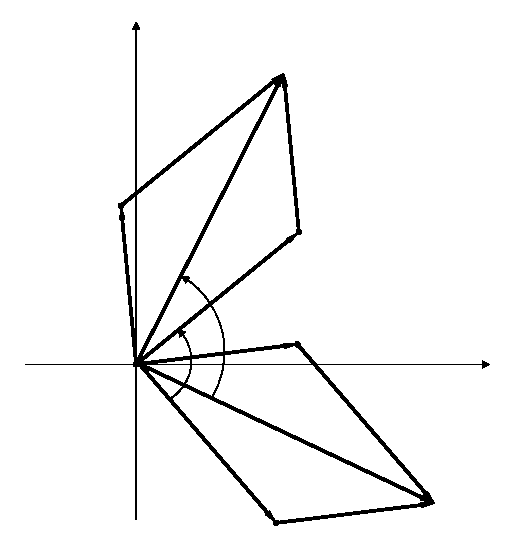
\includegraphics[scale=0.9]{figures/fig1_3_1.pdf}
    \caption{旋转}
\end{figure}

\begin{example*}
    反射：在本例中$V=W=\mathbb{R}^2$，变换$T_{\gamma}:\mathbb{R}^2\to\mathbb{R}^2$是关于第一轴的反射。可以从几何的角度证明该变换为线性的，但我们将用另一种方法来证明。

    方法是：写出$T$的表达式\[T\left(\begin{pmatrix}x_1\\x_2\end{pmatrix}\right)=\begin{pmatrix}x_1\\-x_2\end{pmatrix}\]
    根据该式，我们很容易检验该变换是线性的。
\end{example*}

\begin{example*}
    考察线性变换$T:\mathbb{R}\to\mathbb{R}$。任一此类变换都由下式给出\[T(x)=ax\quad\text{其中}~a=T(1).\]
    的确如此：\[T(x)=T(x\times1)=xT(1)=xa=ax.\]
    因此，$\mathbb{R}$上的任一线性变换仅仅是与常数的乘法。
\end{example*}

\subsection{\texorpdfstring{$\mathbb{F}^n\to \mathbb{F}^m$}{F**n到F**m}的线性变换、矩阵-列向量乘法}

线性变换$T:\mathbb{F}^n\to\mathbb{F}^m$也可用一乘法表示，不过不是与标量相乘，而是与矩阵相乘。

我们来看看是如何乘的。令$T:\mathbb{F}^n\to\mathbb{F}^m$为一线性变换。为了对所有向量$\mathbf{x}\in\mathbb{F}^{n}$计算$T(\mathbf{x})$，我们需要什么信息呢？我的观点是，知道$T$作用于$\mathbb{F}^{n}$中的标准基$\mathbf{e}_1,\mathbf{e}_2,\ldots,\mathbf{e}_n$的结果就足够了。也即，知道$\mathbb{F}^m$中的这$n$个向量（即若干长度为$m$的向量）就足够了：
\[\mathbf{a}_1=T(\mathbf{e}_1),\quad\mathbf{a}_2:=T(\mathbf{e}_2),\quad\ldots,\quad\mathbf{a}_n:=T(\mathbf{e}_n).\]
的确如此：令\[\mathbf{x}=\begin{pmatrix}x_1\\x_2\\\vdots\\x_n\end{pmatrix}.\]
那么$\mathbf{x}=x_{1}\mathbf{e}_{1}+x_{2}\mathbf{e}_{2}+\ldots+x_{n}\mathbf{e}_{n}=\sum_{k=1}^{n}x_{k}\mathbf{e}_{k}$，且有
\[T(\mathbf{x})=T\left(\sum_{k=1}^nx_k\mathbf{e}_k\right)=\sum_{k=1}^nT(x_k\mathbf{e}_k)=\sum_{k=1}^nx_kT(\mathbf{e}_k)=\sum_{k=1}^nx_k\mathbf{a}_k.\]

因此，如果我们将列向量$\mathbf{a}_{1},\mathbf{a}_{2},\ldots,\mathbf{a}_{n}$一起放入一矩阵$A=[\mathbf{a}_1,$ $\mathbf{a}_2,\ldots,\mathbf{a}_n]$（$\mathbf{a}_{k}$是$A$的第$k$列，$k=1,2,\ldots,n$），该矩阵就包含了$T$的所有信息。

下面我们说明如何定义矩阵和列向量的乘积才能将变换$T$表示为乘积$T(\mathbf{x})=A\mathbf{x}$。令
\[A=\begin{pmatrix}a_{1,1}&a_{1,2}&\ldots&a_{1,n}\\a_{2,1}&a_{2,2}&\ldots&a_{2,n}\\\vdots&\vdots&&\vdots\\a_{m,1}&a_{m,2}&\ldots&a_{m,n}\end{pmatrix}.\]

回想一下，$A$的第$k$列是向量$\mathbf{a}_{k}$，即\[\mathbf{a}_k=\begin{pmatrix}a_{1,k}\\a_{2,k}\\\vdots\\a_{m,k}\end{pmatrix}.\]
于是，如果我们要使$A\mathbf{x} = T(\mathbf{x})$，我们就有
\[A\mathbf{x}=\sum_{k=1}^nx_k\mathbf{a}_k=x_1\begin{pmatrix}a_{1,1}\\a_{2,1}\\\vdots\\a_{m,1}\end{pmatrix}+x_2\begin{pmatrix}a_{1,2}\\a_{2,2}\\\vdots\\a_{m,2}\end{pmatrix}+\ldots+x_n\begin{pmatrix}a_{1,n}\\a_{2,n}\\\vdots\\a_{m,n}\end{pmatrix}.\]

因此，矩阵-向量乘法应该按照下述“{\bf 列乘以坐标}”法则来进行：
\begin{center}
    \fbox{将矩阵的各列与向量的对应坐标相乘。}
\end{center}

\begin{example*}
    \[\begin{pmatrix}1&2&3\\3&2&1\end{pmatrix}\begin{pmatrix}1\\2\\3\end{pmatrix}=1\begin{pmatrix}1\\3\end{pmatrix}+2\begin{pmatrix}2\\2\end{pmatrix}+3\begin{pmatrix}3\\1\end{pmatrix}=\begin{pmatrix}14\\10\end{pmatrix}.\]
\end{example*}

“列乘以坐标”法则很适于并行计算，在之后的一些理论推导中也很重要。

不过，当手工进行计算时，逐项计算更为方便。这种计算可按以下“{\bf 行乘以列}”法则来进行：
\begin{center}
    \fbox{\parbox{0.8\linewidth}{要得到结果的第$k$项，我们需要将矩阵的第$k$行与向量相乘。也就是说，若$A\mathbf{x}=\mathbf{y}$，那么$y_{k}=\sum_{j=1}^{n}a_{k,j}x_{j},k=1,2,\ldots, m$。}}
\end{center}
此处$x_j$和$y_k$分别是向量$\mathbf{x}$和$\mathbf{y}$的坐标，$a_{j,k}$则为矩阵$A$的项。

\begin{example*}
    \[\begin{pmatrix}1&2&3\\4&5&6\end{pmatrix}\begin{pmatrix}1\\2\\3\end{pmatrix}=\begin{pmatrix}1\cdot1+2\cdot2+3\cdot3\\4\cdot1+5\cdot2+6\cdot3\end{pmatrix}=\begin{pmatrix}14\\32\end{pmatrix}\]
\end{example*}

\subsection{线性变换与生成组}

我们上面讨论过，从$\mathbb{F}^n$到$\mathbb{F}^m$的线性变换$T$完全决定于其在$\mathbb{F}^n$的标准基上的取值。

其实，我们并不一定要考虑标准基，而是可以考虑任意的基，甚至可以考虑任意生成（张成）组。即
\begin{center}
    \fbox{\parbox{0.8\linewidth}{线性变换$T:V\to W$完全由其在生成组上的取值所决定（特别地，由其在基上的取值所决定）。}}
\end{center}
所以，若$\mathbf{v}_{1},\mathbf{v}_{2},\ldots,\mathbf{v}_{n}$是$V$中的生成组（特别地，若其是$V$的基），并且$T$与$T_1$是线性变换，$T,T_1:V\to W$，使得\[T\mathbf{v}_k=T_1\mathbf{v}_k,\quad k=1,2,\ldots,n\]
那么$T=T_1$。

此结论的证明很简单，留作习题。

\subsection{结论}

\begin{itemize}
    \item 要得到线性变换$T:\mathbb{F}^{n}\to\mathbb{F}^{m}$的矩阵，我们需要将向量$\mathbf{a}_{k}=T\mathbf{e}_{k}$（其中$\mathbf{e}_1,\mathbf{e}_2,\ldots,\mathbf{e}_n$是$\mathbb{F}^n$的标准基）组合成一个矩阵：该矩阵的第$k$列是$\mathbf{a}_{k},k=1,2,\dots,n$。
    \item 若线性变换$T$的矩阵$A$是已知的，那么$T(\mathbf{x})$能通过矩阵-向量乘法$T(\mathbf{x})=A\mathbf{x}$求出。矩阵-向量乘法可用“列乘以坐标”或“行乘以列”法则来运算。
    
    后者更适于手工运算，而前者更适用于并行计算机且将被用于各种理论推导中。
\end{itemize}

对线性变换$T:\mathbb{F}^{n}\to\mathbb{F}^{m}$，其矩阵常记作$[T]$。不过，人们往往不区分线性变换及其矩阵，并常对两者用相同的记号。不致混淆时，我们也会用同样的符号来表示线性变换和其矩阵。

因为线性变换本质上就是乘法，因此常用记号$T\mathbf{v}$而不是$T(\mathbf{v})$表示。我们也会用前者。注意，代数运算的一般顺序仍然适用，也即，$T\mathbf{v}+\mathbf{u}$意为$T(\mathbf{v})+\mathbf{u}$，而非$T(\mathbf{v}+\mathbf{u})$。

\begin{remark*}
    在矩阵-向量乘法$A\mathbf{x}$中，矩阵$A$的列数必须与向量$\mathbf{x}$的长度相同，即$\mathbb{F}^n$中的向量只能被$m\times n$矩阵所乘。

    这是合理的，因为$m\times n$矩阵定义了$\mathbb{F}^n\to\mathbb{F}^m$的线性变换，所以向量$\mathbf{x}$必须属于$\mathbb{F}^n$。

    记住这一点的最简单方法，\marginpar{\small 在用“行乘以列”法则计算矩阵-向量乘法时，确保矩阵的行中的项数和列向量中的项数相同。行中的项和列向量中的项应该被同时用尽；否则所做的乘法未定义。}就是记住如果在做乘法的时候有某种元素先被用光了，那么此乘法就是未定义的。例如，如果用“行乘以列”法则时，你将矩阵的行中各项都用尽了，而列向量中的项仍有未用到的，那么所做的乘法就是未定义的。同样，如果你先用尽列向量中的项，而矩阵的行中各项尚有未用到的，那么该乘法也是未定义的。
\end{remark*}

\begin{remark*}
    不要将自己束缚在$\mathbb{F}^n$及其标准基的情形中：本节陈述的所有内容适用于任意向量空间之间的线性变换——只要定义域和目标空间中都有基。当然，如果基改变了，那么线性变换的矩阵也会相应变化。这将在第 \ref{chap:LinearSystems} 章第 \ref{sec:ChangeOfCoordinate} 节中讨论。
\end{remark*}

\begin{problemset}
    \item 做乘法：
    \begin{probenumerate}
        \item $\begin{pmatrix}1&2&3\\4&5&6\end{pmatrix}\begin{pmatrix}1\\3\\2\end{pmatrix}$；
        \item $\left.\left(\begin{array}{cc}1&2\\0&1\\2&0\end{array}\right.\right)\begin{pmatrix}1\\3\end{pmatrix}$；
        \item $\begin{pmatrix}1&2&0&0\\0&1&2&0\\0&0&1&2\\0&0&0&1\end{pmatrix}\begin{pmatrix}1\\2\\3\\4\end{pmatrix}$；
        \item $\begin{pmatrix}1&2&0\\0&1&2\\0&0&1\\0&0&0\end{pmatrix}\begin{pmatrix}1\\2\\3\\4\end{pmatrix}$。
    \end{probenumerate}
    \item 设$\mathbb{R}^2$上的线性变换为关于直线$x_1=x_2$的反射。求其矩阵。
    \item 对于下述线性变换，求其矩阵：
    \begin{probenumerate}
        \item $T:\mathbb{R}^2\to\mathbb{R}^3$，定义为$T(x,y)^T=(x+2y,2x-5y,7y)^T$；
        \item $T:\mathbb{R}^4\to\mathbb{R}^3$，定义为$T(x_{1},x_{2},x_{3},x_{4})^{T}=(x_{1}+x_{2}+x_{3}+x_{4},x_{2}-x_{4},x_{1}+3x_{2}+6x_{4})^T$；
        \item $T:\mathbb{P}_{n}\to\mathbb{P}_{n},Tf(t)=f^{\prime}(t)$（求其关于标准基$1,t,t^2,\ldots,t^n$的矩阵）；
        \item $T:\mathbb{P}_{n}\to\mathbb{P}_{n},Tf(t)=2f(t)+3f^{\prime}(t)-4f^{\prime\prime}(t)$（仍求其关于标准基$1,t,t^2,\ldots,t^n$的矩阵）。
    \end{probenumerate}
    \item 求出表示下列$\mathbb{R}^3$上的线性变换的$3\times 3$矩阵：
    \begin{probenumerate}
        \item 将所有向量投影至$x$-$y$平面；
        \item 将所有向量关于$x$-$y$平面反射；
        \item 将$x$-$y$平面旋转$30^\circ$，并保持$z$轴不变。
    \end{probenumerate}
    \item 令$A$为线性变换。若$\mathbf{z}$是直线区间$[\mathbf{x},\mathbf{y}]$的中点，证明：$A\mathbf{z}$是区间$[A\mathbf{x},A\mathbf{y}]$的中点。{\bf 提示}：“$\mathbf{z}$是区间$[\mathbf{x},\mathbf{y}]$的中点”意味着什么？
    \item 复数集合$\mathbb{C}$可与向量空间$\mathbb{R}^2$自然对应——视任一$z=x+iy\in\mathbb{C}$为列向量$(x,y)^T\in\mathbb{R}^2$。
    \begin{probenumerate}
        \item 视$\mathbb{C}$为复向量空间，证明与$\alpha=a+ib\in\mathbb{C}$的乘法是$\mathbb{C}$上的线性变换。该变换的矩阵是什么？
        \item 视$\mathbb{C}$为实向量空间$\mathbb{R}^2$，证明与$\alpha=a+ib$的乘法是其上的线性变换。该变换的矩阵是什么？
        \item 定义$T(x+iy)=2x-y+i(x-3y)$。证明：该变换不是复向量空间$\mathbb{C}$上的线性变换，但如果我们把$\mathbb{C}$视为实向量空间$\mathbb{R}^2$，那么该变换是其上的线性变换（即$T$是实线性变换而非复线性变换）。
        
        求出该实线性变换$T$的矩阵。
    \end{probenumerate}
    \item 证明：$\mathbb{C}$（视为复向量空间）中的任意线性变换都是与$\alpha\in\mathbb{C}$的乘法。
\end{problemset}

\section{线性变换作为向量空间的元素}

我们可以对线性变换做什么运算呢？我们总可以将线性变换乘以一标量，也即，设有线性变换$T:V\to W$与标量$\alpha$，我们可定义一新的变换$\alpha T$为
\[(\alpha T)\mathbf{v}=\alpha(T\mathbf{v})\quad\forall\mathbf{v}\in V.\]
容易检验，$\alpha T$亦为线性变换：
\[\begin{aligned}
    (\alpha T)(\alpha_{1}\mathbf{v}_{1}+\alpha_{2}\mathbf{v}_{2})&=\alpha(T(\alpha_{1}\mathbf{v}_{1}+\alpha_{2}\mathbf{v}_{2}))\quad\text{由}~\alpha T~\text{的定义}\\
    &=\alpha(\alpha_{1}T\mathbf{v}_{1}+\alpha_{2}T\mathbf{v}_{2})\quad\text{由}~ T~\text{的线性}\\
    &=\alpha_{1}\alpha T\mathbf{v}_{1}+\alpha_{2}\alpha T\mathbf{v}_{2}=\alpha_{1}(\alpha T)\mathbf{v}_{1}+\alpha_{2}(\alpha T)\mathbf{v}_{2}
\end{aligned}\]

若$T_1$和$T_2$是具有相同的定义域和目标空间的线性变换（$T_{1}:V\to W$并且$T_{2}:V\to W$，或者简写作$T_{1},T_{2}:V\to W$），那么我们可以将这两个线性变换相加，并定义新的变换$T=(T_1+T_2):V\to W$为
\[(T_1+T_2)\mathbf{v}=T_1\mathbf{v}+T_2\mathbf{v}\quad\forall\mathbf{v}\in V.\]
容易检验，变换$T_1+T_2$也是线性的——只需重复上面用于说明$\alpha T$之线性的推理过程即可。

所以，如果我们固定向量空间$V$和$W$，并且考虑所有从$V$到$W$的线性变换所成的集合（将其记为$\mathcal{L}(V,W)$），那么我们可以在$\mathcal{L}(V,W)$上定义两种运算：标量乘法和加法。容易证明，这些运算符合向量空间的所有公理——见第 \ref{sec:vector_space} 节。

读者应该不会对此感到意外，因为向量空间的公理本质上意味着向量的运算符合代数的一般规则，而线性变换的运算的定义天然满足这些规则！

作为演示，我们写出向量空间第一条分配性质（公理7）的正式证明。待证命题是$\alpha(T_{1}+T_{2})=\alpha T_{1}+\alpha T_{2}$。对任意$\mathbf{v}\in V$都有
\[\begin{aligned}
    \alpha(T_{1}+T_{2})\mathbf{v}&=\alpha((T_{1}+T_{2})\mathbf{v})&\text{由乘法的定义}\\
    &=\alpha(T_1\mathbf{v}+T_2\mathbf{v})&\text{由加法的定义}\\
    &=\alpha T_{1}\mathbf{v}+\alpha T_{2}\mathbf{v}&\text{由}~W~\text{的公理7}\\
    &=(\alpha T_{1}+\alpha T_{2})\mathbf{v}&\text{由加法的定义}
\end{aligned}\]
因此，的确有$\alpha(T_{1}+T_{2})=\alpha T_{1}+\alpha T_{2}$。

\begin{remark*}
    适用于线性变换$T:\mathbb{F}^n\to \mathbb{F}^m$的线性运算（加法和标量乘法）与适用于其矩阵的运算相对应。因为我们知道$m\times n$矩阵所成的集合是向量空间，所以立刻可知$\mathcal{L}(\mathbb{F}^n, \mathbb{F}^m)$是向量空间。

    上面我们演示了抽象的证明，原因之一是其适用于一般的空间（例如，不存在基的空间，这种情况我们无法利用坐标来处理），原因之二则是类似于此处抽象证明的推理过程会在许多场合被用到，因此理解它对于读者而言是有益的。

    并且，随着读者愈来愈精通数学，他/她将发现此处的抽象推理其实非常简单——几乎是不假思索就能做出。
\end{remark*}

\section{线性变换的复合与矩阵乘法}

\subsection{矩阵乘法的定义}

在了解矩阵-向量乘法后，很容易猜出两矩阵乘积$AB$的一种自然的定义方式：将$B$的各列乘以$A$（用矩阵-向量乘法），再将所得各列向量组成矩阵。正式而言，
\begin{center}
    \fbox{\parbox{0.8\linewidth}{若$B$的各列是$\mathbf{b}_{1},\mathbf{b}_{2},\ldots,\mathbf{b}_{r}$，那么$A\mathbf{b}_{1},A\mathbf{b}_{2},\ldots,A\mathbf{b}_{r}$是矩阵$AB$的各列。}}
\end{center}
回忆矩阵-向量乘法的“{\bf 行乘以列}”规则，我们得到了下述{\bf 矩阵的}“{\bf 行乘以列}”{\bf 规则}：
\begin{center}
    \fbox{\parbox{0.8\linewidth}{乘积$AB$的项$(AB)_{j,k}$（第$j$行第$k$列中的项）定义为\[(AB)_{j,k}=(A~\text{的第}~j~\text{行})\cdot(B~\text{的第}~k~\text{列})\]}}
\end{center}
正式而言，其可写为\[(AB)_{j,k}=\sum_{l}a_{j,l}b_{l,k},\]
其中$a_{j,k}$和$b_{j,k}$分别表示矩阵$A$和$B$的项。

我特地没说明矩阵$A$和$B$的大小，但是如果我们回想一下矩阵-向量乘法的“行乘以列”规则，我们就能看出，如果一个乘积是有定义的，那么$A$的行的长度应该等于$B$的列的长度。

换言之，乘积$AB$是有定义的，当且仅当$A$是$m\times n$矩阵且$B$是$n\times r$矩阵。

\subsection{缘起：线性变换的复合}

这里，我们不妨问问自己：为什么要用如此复杂的方式定义乘法呢？为什么我们不直接将矩阵逐项相乘呢？

回答是：定义如上的这种乘法，是从线性变换的复合中自然产生的。

假设我们有两个线性变换$T_1:\mathbb{F}^n\to\mathbb{F}^m$和$T_2:\mathbb{F}^r\to\mathbb{F}^n$。定义线性变换$T_1,T_2$的复合$T=T_1\circ T_2$为\[T(\mathbf{x})=T_1(T_2(\mathbf{x}))\quad\forall \mathbf{x}\in\mathbb{F}^r.\]
注意$T_{2}(\mathbf{x})\in\mathbb{F}^{n}$。由于$T_{1}:\mathbb{F}^{n}\to\mathbb{F}^{m}$，所以表达式$T_1(T_2(\mathbf{x}))$是定义完善的，且变换后的结果属于$\mathbb{F}^m$。因此$T:\mathbb{F}^{r}\to\mathbb{F}^{m}$。

容易证明，\marginpar{\small 我们通常会把线性变换与其矩阵等同起来看，不过在下面几段中我们会将它们区分开。}$T$是线性变换（留作习题），因此其由一$m\times r$矩阵所确定。如何在已知$T_1$和$T_2$的矩阵的情况下求出这个矩阵呢？

令$A$是$T_1$的矩阵，$B$是$T_2$的矩阵。在之前的小节中我们讨论过，$T$的各列是向量$T(\mathbf{e}_{1}),T(\mathbf{e}_{2}),\ldots,T(\mathbf{e}_{r})$，其中$\mathbf{e}_1,\mathbf{e}_2,\ldots,\mathbf{e}_r$是$\mathbb{F}^r$的标准基。对$k=1,2,\ldots,r$我们有\[T(\mathbf{e}_k)=T_1(T_2(\mathbf{e}_k))=T_1(B\mathbf{e}_k)=T_1(\mathbf{b}_k)=A\mathbf{b}_k\]
（变换$T_2$和$T_1$分别是与$B$和$A$做乘法）

因此，$T$的矩阵各列是$A\mathbf{b}_{1},A\mathbf{b}_{2},\ldots,A\mathbf{b}_{r}$，而这就是矩阵$AB$的定义！

我们重新将线性变换与其矩阵等同起来看。由于矩阵乘法与线性变换的复合是一致的，我们可以（并且将要）用$T_1T_2$这种写法取代$T_1\circ T_2$，并且用$T_{1}T_{2}\mathbf{x}$这种写法取代$T_{1}(T_{2}(\mathbf{x}))$。

注意，在复合$T_1T_2$中，\marginpar{\small {\bf 注意}：变换的顺序！}首先作用的是变换$T_2$！记住这一点的方法是，注意到在$T_1T_2\mathbf{x}$中，首先碰上$\mathbf{x}$的是变换$T_2$。

\begin{remark*}
    除“行乘以列”法则以外，还有一种检验矩阵乘积中各矩阵大小的方法：要使复合$T_1T_2$有定义，$T_2\mathbf{x}$必须属于$T_1$的定义域。若$T_2$从某个空间（比如说$\mathbb{F}^r$）映射到$\mathbb{F}^n$，那么$T_1$一定要从$\mathbb{F}^n$映射到某个空间（比如说$\mathbb{F}^m$）。所以，要使$T_1T_2$有定义，$T_1$和$T_2$的矩阵的大小必须分别是$m\times n$和$n\times r$——这和我们由“{\bf 行乘以列}”法则所得到的条件是一样的。
\end{remark*}

\begin{example*}
    令$T:\mathbb{R}^{2}\to\mathbb{R}^{2}$是关于直线$x_1=3x_2$的反射。它是线性变换，现在来求其矩阵。要求这个矩阵，我们需计算$T\mathbf{e}_{1}$和$T\mathbf{e}_{2}$。然而，直接计算$T\mathbf{e}_{1}$和$T\mathbf{e}_{2}$所需的三角学知识远远超出了一个正常人愿意记忆的范畴。

    $T$的矩阵的一个更为简便的求法是，将$T$表示成若干简单线性变换的复合。具体而言，令$\gamma$为$x_1$轴和直线$x_1=3x_2$之间的夹角，并令$T_0$为沿$x_1$轴的反射。那么，要得到反射$T$，我们可以首先将平面旋转$-\gamma$以将直线$x_1=3x_2$转到$x_1$轴上，然后将向量沿$x_1$轴反射，最后将平面旋转$\gamma$以恢复原状。正式而言，这三步可以写成
    \[T=R_\gamma T_0R_{-\gamma}\]
    （注意各项的顺序！）其中$R_\gamma$表示旋转$\gamma$弧度。$T_0$的矩阵很容易计算：
\[T_0=\begin{pmatrix}1&0\\0&-1\end{pmatrix},\]
而旋转矩阵是我们已知的：
\[\begin{aligned}
    R_{\gamma}&=\begin{pmatrix}{\cos\gamma}&{-\sin\gamma}\\{\sin\gamma}&{\cos\gamma}\end{pmatrix},\\
    R_{-\gamma}&=\left(\begin{array}{cc}{\cos(-\gamma)}&{-\sin(-\gamma)}\\{\sin(-\gamma)}&{\cos(-\gamma)}\end{array}\right)=\begin{pmatrix}{\cos\gamma}&{\sin\gamma}\\{-\sin\gamma}&{\cos\gamma}\end{pmatrix}\end{aligned}
\]
为计算$\sin\gamma$和$\cos\gamma$，可在直线$x_1=3x_2$上取一向量，比如向量$(3,1)^T$。那么\[\cos\gamma=\frac{\text{第一个坐标}}{\text{长度}}=\frac{3}{\sqrt{3^2+1^2}}=\frac{3}{\sqrt{10}}\]
类似地\[\sin\gamma=\frac{\text{第二个坐标}}{\text{长度}}=\frac{1}{\sqrt{3^2+1^2}}=\frac{1}{\sqrt{10}}\]
将上面这些组合起来可得
\[\begin{aligned}T=R_{\gamma}T_{0}R_{-\gamma}&=\frac{1}{\sqrt{10}}\begin{pmatrix}{3}&{-1}\\{1}&{3}\end{pmatrix}\begin{pmatrix}{1}&{0}\\{0}&{-1}\end{pmatrix}\frac{1}{\sqrt{10}}\begin{pmatrix}{3}&{1}\\{-1}&{3}\end{pmatrix}\\&=\frac{1}{10}\begin{pmatrix}3&-1\\1&3\end{pmatrix}\begin{pmatrix}1&0\\0&-1\end{pmatrix}\begin{pmatrix}3&1\\-1&3\end{pmatrix}\end{aligned}\]
只需计算矩阵乘法，即可得到最终结果。
\end{example*}

\subsection{矩阵乘法的性质}

矩阵乘法有许多性质，而这些性质我们在高中代数课就已熟悉：
\begin{enumerate}
    \item 结合律：$A(BC)=(AB)C$——前提是左侧或右侧的乘积都是定义完善的。从而我们就能（并且将会）把这种情况简记作$ABC$。
    \item 分配律：$A(B+C)=AB+AC,(A+B)C=AC+BC$——前提是左侧或右侧的乘积都是定义完善的。
    \item 标量可以提出：$A(\alpha B)=(\alpha A)B=\alpha(AB)=\alpha AB$。
\end{enumerate}
这些性质很容易证明。你应该证明线性变换的对应性质——由定义即很容易得到，然后再由线性变换的这些性质推出矩阵乘法的对应性质。

此处新出现的难点是，交换律不成立：
\begin{quote}
    矩阵乘法是不可交换的，即一般来说$AB\ne BA$。
\end{quote}
容易看出，期望矩阵乘法的交换律成立是不合理的。的确如此：令$A$和$B$分别为$m\times n$和$n\times r$矩阵。那么乘积$AB$是定义完善的，但若$m\ne r$则$BA$是未定义的。

即便两个乘积都有定义，比如说$A$和$B$都是$n\times n$方阵的情况，乘法仍然不是可交换的。如果我们随机选择矩阵$A$和$B$，那么大概率$AB\ne BA$，运气很好的时候才会恰巧得到$AB=BA$的结果。

\subsection{转置矩阵与乘法}

简单分析“行乘以列”规则可得\[(AB)^{T}=B^{T}A^{T},\]
即，当对乘积取转置时，需更改各项的顺序。\footnote{原书中本节的大多数内容在 \ref{subsec:matrix_notation} 节中已经陈述过了，此处将重复的部分略去。——译者注}

\subsection{迹与矩阵乘法}

对于方阵（$n\times n$矩阵）$A=(a_{j,k})$，其迹（记为$\tr A$）是对角线项之和：
\[\operatorname{trace}A=\sum_{k=1}^{n}a_{k,k}.\]
\begin{theorem}\label{thm:trace_commute}
    令$A$和$B$分别为$m\times n$和$n\times m$矩阵（则乘积$AB$和$BA$都是定义完善的）。那么\[\tr (AB)=\tr(BA)\]
\end{theorem}
此定理的证明留作习题（见下习题 \ref{ex:1_5_6}）。其实，这个定理有两种证法。第一种方法是计算$AB$与$BA$的对角线项并比较两者的和。这种方法对于操作嵌套的求和有较高的要求。

如果你不擅长代数运算，还可用另一种方法。我们可以考虑两个从$M_{n\times m}$到$\mathbb{F}=\mathbb{F}^1$的线性变换$T$和$T_1$，定义为：\[T(X)=\mathrm{trace}(AX),\quad T_{1}(X)=\mathrm{trace}(XA)\]
只需证明$T=T_1$即可得证——代入$X=B$可得到原定理。

由于线性变换完全由其在生成组上的取值所决定，我们只需对一些简单的矩阵检验$T=T_1$——比如考虑矩阵$X_{j,k}$，其中除了第$j$列第$k$行的项为$1$外，其余各项均为$0$。

\begin{problemset}
    \item 令
    \[A=\begin{pmatrix}1&2\\3&1\end{pmatrix},B=\begin{pmatrix}1&0&2\\3&1&-2\end{pmatrix},C=\begin{pmatrix}1&-2&3\\-2&1&-1\end{pmatrix},D=\begin{pmatrix}-2\\2\\1\end{pmatrix}\]
    \begin{probenumerate}
        \item 选出所有有定义的乘积，并给出乘积的大小：$AB,BA,ABC,ABD,BC,$ $BC^{T},B^{T}C,DC,D^{T}C^{T}.$
        \item 计算$AB,A(3B+C),B^{T}A,A(BD),(AB)D.$
    \end{probenumerate}
    \item 令$T_\gamma$为$\mathbb{R}^2$中旋转$\gamma$弧度的矩阵。用矩阵乘法检验$T_{\gamma}T_{-\gamma}=T_{-\gamma}T_{\gamma}=I$。
    \item 将两个旋转矩阵$T_{\alpha}$和$T_{\beta}$相乘（该乘法是罕见的可交换乘法，即$T_\alpha T_\beta=T_\beta T_\alpha$，故顺序不重要）。据此推导$\sin(\alpha+\beta)$和$\cos(\alpha+\beta)$的公式。
    \item 求出$\mathbb{R}^2$中向直线$x_1=-2x_2$上正交投影的矩阵。{\bf 提示}：向坐标轴$x_1$上投影的矩阵是什么？
    \item 求出线性变换$A,B:\mathbb{R}^{2}\to\mathbb{R}^{2}$使得$AB=\mathbf{0}$但$BA\ne \mathbf{0}$。
    \item \label{ex:1_5_6}证明定理 \ref{thm:trace_commute}，即证明$\tr (AB)=\tr(BA)$。
    \item 构造非零矩阵$A$使得$A^{2}=\mathbf{0}$。
    \item 求出关于直线$y=-2x/3$的反射的矩阵。请将所有乘法都算到最终结果。
\end{problemset}

\section{可逆变换与矩阵、同构}

\subsection{恒等变换和恒等矩阵}

在所有线性变换中，有个很特殊的线性变换——恒等变换（恒等算子）$I$，$I\mathbf{x}=\mathbf{x},\forall\mathbf{x}$。

准确地说，恒等变换有无数多个：对任意向量空间$V$，都有一个恒等变换$I=I_{V}:V\to V,I_{V}\mathbf{x}=\mathbf{x},\forall\mathbf{x}\in V$。然而，不致混淆时，我们将用同一符号$I$表示所有的恒等算子（恒等变换）。只有在强调该变换作用于哪个空间时，我们才用记号$I_V$。

显然，\marginpar{\small 通常，线性代数教材中用符号$E$表示恒等矩阵。我更中意$I$，因为在算子理论中用的是它。}如果$I:\mathbb{F}^n\to\mathbb{F}^n$是$\mathbb{F}^n$上的恒等变换，则其矩阵为$n\times n$矩阵\[I=I_n=\begin{pmatrix}1&0&\ldots&0\\0&1&\ldots&0\\\vdots&\vdots&\ddots&\vdots\\0&0&\ldots&1\end{pmatrix}\]
（主对角线上全为$1$，而其余地方全为$0$）。当我们需要强调矩阵的大小时，就用$I_n$做个记号；否则我们用$I$即可。

显然，对于任意线性变换$A$，等式\[AI=A,\quad IA=A\]成立（只要乘积是有定义的）。

\subsection{可逆变换}

\begin{definition*}
    令$A:V\to W$为一线性变换。称变换$A$是{\bf 左可逆的}，若存在线性变换$B:W\to V$使得\[BA=I\quad(\text{此处}~I=I_{V}).\]
    称变换$A$是{\bf 右可逆的}，若存在线性变换$C:W\to V$使得\[AC=I\quad(\text{此处}~I=I_{W}).\]
    线性变换$B$和$C$分别称为$A$的{\bf 左逆}和{\bf 右逆}。注意，我们并没有假设$B$和$C$的唯一性，并且通常左逆和右逆也不是唯一的。
\end{definition*}

\begin{definition*}
    称线性变换$A:V\to W$是{\bf 可逆的}，若其既是左可逆的又是右可逆的。
\end{definition*}

\begin{theorem}\label{thm:inverse_unique}
    若线性变换$A:V\to W$是可逆的，那么其左逆$B$和右逆$C$是唯一且相等的。
\end{theorem}

\begin{corollary*}
    线性变换$A:V\to W$是可逆的，\marginpar{\small 这条性质往往被用作可逆线性变换的定义。}当且仅当存在唯一的线性变换（记为$A^{-1}$），$A^{-1}:W\to V$使得\[A^{-1}A=I_V,\quad AA^{-1}=I_W.\]
    变换$A^{-1}$称作$A$的{\bf 逆}。
\end{corollary*}

\begin{proof}[定理 \ref{thm:inverse_unique} 的证明]
    令$BA=I$且$AC=I$。那么\[BAC=B(AC)=BI=B.\]
    另一方面，\[BAC=(BA)C=IC=C,\]
    因此$B=C$。

    假设对于某个线性变换$B_1$有$B_1A=I$。将上面对$B$所做的推理作用于$B_1$，可得$B_1=C$。因此，左逆$B$是唯一的。类似可证$C$的唯一性。
\end{proof}

\begin{definition*}
    称矩阵是{\bf 可逆的}（意即{\bf 左可逆}且{\bf 右可逆}），如果相应的线性变换是可逆的（意即{\bf 左可逆}且{\bf 右可逆}）。
\end{definition*}

定理 \ref{thm:inverse_unique} 表明若存在唯一的矩阵$A^{-1}$使得$A^{-1}A=I,AA^{-1}=I$，则矩阵$A$是可逆的。矩阵$A^{-1}$称作$A$的{\bf 逆}。

\subsubsection*{例子}

\begin{enumerate}
    \item 恒等变换（恒等矩阵）是可逆的，$I^{-1} = I$；
    \item 旋转$R_\gamma$\[R_\gamma=\begin{pmatrix}\cos\gamma&-\sin\gamma\\\sin\gamma&\cos\gamma\end{pmatrix}\]
    是可逆的，且其逆为$(R_{\gamma})^{-1}=R_{-\gamma}$。从$R_\gamma$的几何描述很容易得到该等式，也可以通过矩阵乘法来检验它。
    \item 列向量$(1,1)^T$是左可逆的但不是右可逆的。其左逆可以是行向量$(1/2,1/2)$。
    
    为了说明该矩阵不是右可逆的，只需注意到该矩阵存在不止一个左逆。{\bf 习题}：描述该矩阵的所有左逆。
    \item 行向量$(1,1)$是右可逆的，但不是左可逆的。可能的右逆之一是列向量$(1/2,1/2)^T$。
\end{enumerate}

\begin{remark}
    可逆矩阵{\bf 必为}方阵（$n\times n$）。此外，若方阵$A$有左逆或右逆，那么其为可逆 的。因此，只需检验等式$AA^{-1}=I,A^{-1}A=I$其中之一。

    该结论会在后面证明。在证明该结论之前，我们将不会使用它。我在此处先提及它只是为了防止学生误入歧途。
\end{remark}

\subsubsection{逆变换的性质}

\begin{theorem}[乘积的逆]
    若线性变换$A$和$B$是可逆的（并且乘积$AB$是有定义的），那么乘积$AB$是可逆的，且\[(AB)^{-1}=B^{-1}A^{-1}\]
    （注意顺序的变化！）
\end{theorem}
\begin{proof}
    直接计算有\[(AB)(B^{-1}A^{-1})=A(BB^{-1})A^{-1}=AIA^{-1}=AA^{-1}=I\]
    类似地\[(B^{-1}A^{-1})(AB)=B^{-1}(A^{-1}A)B=B^{-1}IB=B^{-1}B=I\]
\end{proof}

\begin{remark}
    乘积$AB$的可逆性并不蕴涵$A$和$B$的可逆性（你能举出一个例子吗？）。然而，如果因子之一（$A$或$B$）是可逆的，且乘积$AB$可逆，那么另一个因子也是可逆的。

    我们将这一结论的证明留作习题。
\end{remark}

\begin{theorem}[$A^T$的逆]
    若矩阵$A$可逆，那么$A^T$也可逆，且\[(A^T)^{-1}=(A^{-1})^T\]
\end{theorem}
\begin{proof}
    利用$(AB)^{T}=B^{T}A^{T}$，我们有\[(A^{-1})^TA^T=(AA^{-1})^T=I^T=I,\]
    类似地，\[A^T(A^{-1})^T=(A^{-1}A)^T=I^T=I.\]
\end{proof}
最后，若$A$可逆，那么$A^{-1}$也可逆，且$(A^{-1})^{-1}=A$。

让我们总结逆的主要性质：
\begin{enumerate}
    \item 若$A$可逆，那么$A^{-1}$也可逆，且$(A^{-1})^{-1}=A$；
    \item 若$A$和$B$是可逆的，并且乘积$AB$是有定义的，那么$AB$是可逆的，且$(AB)^{-1}=B^{-1}A^{-1}$；
    \item 若$A$可逆，那么$A^T$也可逆，且$(A^T)^{-1}=(A^{-1})^T$。
\end{enumerate}

\subsection{同构、同构向量空间}

称可逆线性变换$A:V\to W$为{\bf 同构}。我们并未引入任何新概念，只是给我们已研究过的对象取了一个新名字而已。

称两个向量空间$V$和$W$是{\bf 同构的}（记作$V\cong W$），若存在同构$A:V\to W$。

同构的向量空间可视作同一向量空间的不同表达，意即涉及向量空间运算的所有性质和推导在同构下都是保持不变的。

以下定理形象展示了这一说法。

\begin{theorem}\label{thm:preserve_basis}
    令$A:V\to W$是同构，并令$\mathbf{v}_1,\mathbf{v}_2,\ldots,\mathbf{v}_n$是$V$的基。那么向量组$A\mathbf{v}_{1},A\mathbf{v}_{2},\ldots,A\mathbf{v}_{n}$是$W$的基。
\end{theorem}

此定理的证明留作习题。

\begin{remark*}
    可以将上述定理中的“基”换成“线性无关组”、“生成组”或“线性相关组”——所有这些性质在同构下都是保持不变的。
\end{remark*}

\begin{remark*}
    若$A$为同构，那么$A^{-1}$也是同构。因此我们可以把上述定理表述成$\mathbf{v}_1,\mathbf{v}_2,\ldots,\mathbf{v}_n$是基当且仅当$A\mathbf{v}_{1},A\mathbf{v}_{2},\ldots,A\mathbf{v}_{n}$是基。
\end{remark*}

定理 \ref{thm:preserve_basis} 的逆命题也是成立的。

\begin{theorem}\label{thm:basis_to_basis}
    令$A:V\to W$是线性映射，并令$\mathbf{v}_1,\mathbf{v}_2,\ldots,\mathbf{v}_n$和$\mathbf{w}_1,\mathbf{w}_2,\ldots,$ $\mathbf{w}_n$分别为$V$和$W$的基。若$A\mathbf{v}_{k}=\mathbf{w}_{k},k=1,2,\dots,n$，那么$A$是同构。
\end{theorem}
\begin{proof}
    定义逆变换$A^{-1}$为$A^{-1}\mathbf{w}_{k}=\mathbf{v}_{k},k=1,2,\dots,n$（我们知道，线性变换由其在基上的取值所决定）。
\end{proof}

\subsubsection*{例子}

\begin{enumerate}
    \item 令$A:\mathbb{F}^{n+1}\to\mathbb{P}_{n}^{\mathbb{F}}$（$\mathbb{P}_{n}^{\mathbb{F}}$是次数最高为$n$的多项式$\sum_{k=0}^{n}\alpha_{k}t^{k},\alpha_{k}\in\mathbb{F}$所成的集合）定义为\[A\mathbf{e}_1=1,A\mathbf{e}_2=t,\ldots,A\mathbf{e}_n=t^{n-1},A\mathbf{e}_{n+1}=t^n\]
    由定理 \ref{thm:basis_to_basis}，$A$为同构，故$\mathbb{P}_n^\mathbb{F}\cong\mathbb{F}^{n+1}$。
    \item 令$V$为$\mathbb{F}$上的向量空间，\marginpar{\small 任一具有基的实向量空间都与$\mathbb{R}^n$（$n$为适当的数）同构。类似地，任一具有基的复向量空间都与$\mathbb{C}^n$同构。}基为$\mathbf{v}_{1},\mathbf{v}_{2},\ldots,\mathbf{v}_{n}$。定义变换$A:\mathbb{F}^{n}\to V$为\[A\mathbf{e}_k=\mathbf{v}_k,\quad k=1,2,\ldots,n,\]
    其中$\mathbf{e}_1,\mathbf{e}_2,\ldots,\mathbf{e}_n$是$\mathbb{F}^n$的标准基。同样由定理 \ref{thm:basis_to_basis}，$A$为同构，故$V\cong\mathbb{F}^{n}$。
    \item 由$2\times 3$矩阵（各项属于$\mathbb{F}$）所构成的向量空间$M_{2\times3}^{\mathrm{F}}$同构于$\mathbb{F}^6$；
    \item 更一般地，$M_{m\times n}^{\mathbb{F}}\cong\mathbb{F}^{m\cdot n}$。
\end{enumerate}

\subsection{可逆性与方程}\label{subsec:invert_eq}

\begin{theorem}\label{thm:invert_unique}
    令$A:X\to Y$为线性变换。\marginpar{\small 这是不是让你想起了基？}那么$A$可逆，当且仅当对任意右端项$\mathbf{b}\in Y$，方程\[A\mathbf{x}=\mathbf{b}\]有唯一解$\mathbf{x}\in X$。
\end{theorem}
\begin{proof}
    设$A$是可逆的。那么$\mathbf{x}=A^{-1}\mathbf{b}$是方程$A\mathbf{x}=\mathbf{b}$的解。为证明该解是可逆的，设另一向量$\mathbf{x}_1\in X$满足\[A\mathbf{x}_1=\mathbf{b}\]
    将此等式两端左乘$A^{-1}$，可得\[A^{-1}A\mathbf{x}_{1}=A^{-1}\mathbf{b},\]
    因此$\mathbf{x}_{1}=A^{-1}\mathbf{b}=\mathbf{x}$。注意，$AA^{-1}=I$和$A^{-1}A=I$这两个等式都用到了。

    现在假设方程$A\mathbf{x}=\mathbf{b}$对于任意$\mathbf{b}\in Y$有唯一解。下面用符号$\mathbf{y}$而不用$\mathbf{b}$。我们知道，给定$\mathbf{y}\in Y$，方程\[A\mathbf{x}=\mathbf{y}\]有唯一解$\mathbf{x}\in X$。记此解为$B(\mathbf{y})$。

    注意$B(\mathbf{y})$对于所有$\mathbf{y}\in Y$都有定义，因此我们定义了一个变换$B:Y\to X$。

    下面检验$B$是线性变换。我们需要证明$B(\alpha\mathbf{y}_{1}+\beta\mathbf{y}_{2})=\alpha B(\mathbf{y}_{1})+\beta B(\mathbf{y}_{2})$。令$\mathbf{x}_{k}:=B(\mathbf{y}_{k}),k=1,2$，即$A\mathbf{x}_{k}=\mathbf{y}_{k},k=1,2$。那么\[A(\alpha\mathbf{x}_1+\beta\mathbf{x}_2)=\alpha A\mathbf{x}_1+\beta A\mathbf{x}_2=\alpha\mathbf{y}_1+\beta\mathbf{y}_2,\]
    这表明\[B(\alpha\mathbf{y}_1+\beta\mathbf{y}_2)=\alpha B(\mathbf{y}_1)+\beta B(\mathbf{y}_2).\]

    最后，我们证明$B$的确是$A$的逆。取$\mathbf{x}\in X$并令$\mathbf{y}=A\mathbf{x}$，则根据$B$的定义，我们有$\mathbf{x}=B\mathbf{y}$。那么对所有$\mathbf{x}\in X$有\[BA\mathbf{x}=B\mathbf{y}=\mathbf{x},\]
    故$BA=I$。类似地，对任意$\mathbf{y}\in Y$令$\mathbf{x}=B\mathbf{y}$，故$\mathbf{y}=A\mathbf{x}$。则对所有$\mathbf{y}\in Y$均有\[AB\mathbf{y}=A\mathbf{x}=\mathbf{y},\]
    故$AB=I$。
\end{proof}

回忆一下基的定义，我们可得定理 \ref{thm:preserve_basis} 和 \ref{thm:basis_to_basis} 的如下推论。

\begin{corollary}\label{cor:invert_basis}
    $m\times n$矩阵是可逆的，当且仅当它的列形成$\mathbb{F}^m$的基。
\end{corollary}

\begin{problemset}
    \item 证明：若$A:V\to W$是同构（即可逆线性变换），且$\mathbf{v}_1,\mathbf{v}_2,\ldots,\mathbf{v}_n$是$V$的基。那么$A\mathbf{v}_{1},A\mathbf{v}_{2},\ldots,A\mathbf{v}_{n}$是$W$的基。
    \item 求出$1\times 2$矩阵（行向量）$A=(1,1)$的所有右逆，并由此得出结论：行向量$A$不是左可逆的。
    \item 求出列向量$(1,2,3)^T$的所有左逆。
    \item 列向量$(1,2,3)^T$是右可逆的吗？论证之。
    \item 找出两个矩阵$A$和$B$，满足$AB$是可逆的，但$A$和$B$不是。{\bf 提示}：方阵$A$和$B$并不能用于举例。{\bf 注}：在$AB$是$1\times 1$矩阵（标量）时，很容易构造$A$和$B$。但你能否对于$AB$为$2\times 2$矩阵的情况进行构造？$3\times 3$和$n\times n$呢？
    \item 设乘积$AB$可逆。证明：$A$是右可逆的且$B$是左可逆的。{\bf 提示}：写出右逆和左逆的表达式。
    \item 设$A$和$AB$都可逆（假设乘积$AB$是定义完善的）。证明：$B$是可逆的。
    \item 设$A$是$n\times n$矩阵。证明：若$A^2=\mathbf{0}$，那么$A$不可逆。
    \item 设$AB=\mathbf{0}$对某非零矩阵$B$成立。$A$可能是可逆的吗？论证之。
    \item 写出$\mathbb{F}^5$中线性变换$T_1$和$T_2$的矩阵。这两个变换的定义是：$T_1$将向量$\mathbf{x}$的坐标$x_2$和$x_4$互换，而$T_2$将$x_4$的$a$倍加到$x_2$，并不改变其他坐标，即
    \[T_1\begin{pmatrix}x_1\\x_2\\x_3\\x_4\\x_5\end{pmatrix}=\begin{pmatrix}x_1\\x_4\\x_3\\x_2\\x_5\end{pmatrix},\quad T_2\begin{pmatrix}x_1\\x_2\\x_3\\x_4\\x_5\end{pmatrix}=\begin{pmatrix}x_1\\x_2+ax_4\\x_3\\x_4\\x_5\end{pmatrix};\]
    此处$a$为某固定的数。

    证明：$T_1$和$T_2$是可逆变换，并写出它们的逆的矩阵。{\bf 提示}：比起猜想（或计算）$T_1,T_2$这两个矩阵的逆，先描述出逆变换再求出逆变换的矩阵可能更为容易。
    \item 求出$\mathbb{R}^3$中绕向量$(1,2,3)^T$旋转$\alpha$角度这一变换的矩阵。我们假设从向量的尾端看向原点时，所做的旋转为逆时针方向。
    
    你可以将答案写成若干矩阵相乘的形式，而不需要将所有乘法都算到最后。
    \newpage
    \item 给出满足下面条件的矩阵（比如$2\times 2$矩阵）的例子：
    \begin{probenumerate}
        \item $A+B$不可逆，尽管$A$和$B$都可逆；
        \item $A+B$可逆，尽管$A$和$B$都不可逆；
        \item $A$、$B$、$A+B$都可逆。
    \end{probenumerate}
    \item 令$A$为可逆的对称矩阵（$A^T=A$）。$A$的逆还是对称的吗？论证之。
\end{problemset}

\section{子空间}\label{sec:subspace}

向量空间$V$的{\bf 子空间}是$V$的非空子集$V_0\subset V$，它对于向量加法和标量乘法都是封闭的，也即：
\begin{enumerate}
    \item 若$\mathbf{v}\in V_0$，那么对于所有标量$\alpha$都有$\alpha \mathbf{v}\in V_0$；
    \item 对于任意$\mathbf{u},\mathbf{v}\in V_0$，都有求和结果$\mathbf{u}+\mathbf{v}\in V_0$；
\end{enumerate}

同样，这两个条件可替换成下面这一个：
\begin{center}
    对于所有标量$\alpha,\beta$和所有$\mathbf{u},\mathbf{v}\in V_0$，都有$\alpha\mathbf{u}+\beta\mathbf{v}\in V_0$。
\end{center}

注意，具有继承自$V$的运算（向量加法和标量乘法）的子空间$V_0\subset V$是向量空间。的确如此：由于$V$非空，它至少包含一个向量$\mathbf{v}$，又因为$\mathbf{0}=0\mathbf{v}$，上述条件1表明零向量$\mathbf{0}$属于$V$。并且对于任意$\mathbf{v}\in V$，其加法逆元$-\mathbf{v}$由$-\mathbf{v}=(-1)\mathbf{v}$给出，所以同样由性质1可得$-\mathbf{v}\in V$。向量空间的其余公理也都成立，因为所有运算都继承自$V$。唯一可能出问题的一点，就是运算的结果可能不属于$V_0$。但是子空间的定义规避了这种情况！

现在我们考虑一些例子：
\begin{enumerate}
    \item 向量空间$V$的{\bf 平凡}子空间，即$V$自身和$\{\mathbf{0}\}$（仅包含零向量的子空间）。注意，空集$\varnothing$不是向量空间（因为不包含零向量），因此它不是子空间。
\end{enumerate}
对于每个线性变换$A:V\to W$，有以下两个子空间与之关联：
\begin{enumerate}[start=2]
    \item $A$的{\bf 零空间}或{\bf 核}，记为$\nul A$或$\ker A$，由所有满足$A\mathbf{v}=\mathbf{0}$的向量$\mathbf{v}\in V$所构成。
    \item \textbf{值域}$\rg A$定义为由所有可被表示成$\mathbf{w}=A\mathbf{v}$（其中$\mathbf{v}\in V$）的向量$\mathbf{w}\in W$所构成的集合。
\end{enumerate}
若$A$为矩阵，即$A:\mathbb{F}^m\to\mathbb{F}^n$，回想一下矩阵-向量乘法的“{\bf 列乘以坐标}”规则，我们可看出，任意向量$\mathbf{w}\in \rg A$可表示成矩阵$A$各列的线性组合。这就能解释为何常使用列空间（记号为$\col A$）这个术语来指代矩阵的值域。因此，对于矩阵$A$，更常用记号$\col A$而非$\rg A$。

最后一个例子是：
\begin{enumerate}[start=4]
    \item 给定向量组$\mathbf{v}_{1},\mathbf{v}_{2},\ldots,\mathbf{v}_{r}\in V$，其{\bf 线性张成空间}（有时可简称为{\bf 张成空间}）$\mathcal{L}\{\mathbf{v}_{1},\mathbf{v}_{2},\ldots,\mathbf{v}_{r}\}$是可被表示为$\mathbf{v}_{1},\mathbf{v}_{2},\ldots,\mathbf{v}_{r}$的线性组合$\mathbf{v}=\alpha_{1}\mathbf{v}_{1}+\alpha_{2}\mathbf{v}_{2}+\ldots+\alpha_{r}\mathbf{v}_{r}$的所有向量$\mathbf{v}\in V$所构成的集合。除$\mathcal{L}\{\mathbf{v}_{1},\mathbf{v}_{2},\ldots,\mathbf{v}_{r}\}$外，也用记号$\operatorname{span}\{\mathbf{v}_{1},\mathbf{v}_{2},\ldots,\mathbf{v}_{r}\}$来表示。
\end{enumerate}
容易检验，这些例子中的向量空间的确是子空间——留给读者作为习题。其中有些结论会在后文得到证明。

\begin{problemset}
    \item 令$X$和$Y$是向量空间$V$的子空间。证明$X\cap Y$是$V$的子空间。
    \item 令$V$是向量空间。对于$X,Y\subset V$，$X+Y$是所有可被表示为$\mathbf{v}=\mathbf{x}+\mathbf{y},\mathbf{x}\in X,\mathbf{y}\in Y$的向量$\mathbf{v}$所构成的集合。证明若$X$和$Y$是$V$的{\bf 子空间}，那么$X+Y$也是$V$的子空间。
    \item 令$X$是向量空间$V$的子空间，并令$\mathbf{v}\in V,\mathbf{v}\notin X$。证明：若$\mathbf{x}\in X$则$\mathbf{x}+\mathbf{v}\not\in X$。
    \item 令$X$和$Y$是向量空间$V$的子空间。利用上一题的结论证明：$X\cup Y$是子空间，当且仅当$X\subset Y$或$Y\subset X$。
    \item 由$4\times 4$矩阵所构成的空间的所有子空间里，包含所有上三角矩阵（对于所有$j>k$有$a_{j,k}=0$）的最小子空间是什么？包含所有对称矩阵（$A^T=A$）的最小子空间是什么？这两个子空间所共同包含的最大子空间是什么？
\end{problemset}

\section{在计算机图形学中的应用}

本节我们给出线性代数在计算机图形学中的一些实际应用。我们并不会深究细节，而只是陈述一些基本思想。我们会重点解释为什么对于$3$维图像的运算可简化为$4\times 4$矩阵的乘法。

\subsection{\texorpdfstring{$2$}{2}维图形}

计算机显示屏可建模为$x$-$y$平面（更准确地说，其中的一个矩形）。显示屏上出现的任意图形都可用一系列{\bf 像素}来表示，而每个像素都被赋予了特定的颜色。每个像素的位置都由行号和列号所确定，二者充当了平面上$x$和$y$坐标的角色。因此，用带$x$-$y$坐标的平面中的矩形来表示计算机屏幕是很合适的——而一个图形只不过是一系列点。

\begin{remark*}
    图形分为两类：位图（会给出每个像素的信息）和矢量图（只给出{\bf 关键点}的信息，而绘图引擎将这些点连接起来以重构出完整图形）。位图的一个很好的例子是（数字）相片：其中每个像素都会被描述。位图可能包含大量的点，因此对于位图进行运算需要大量的算力。用位图处理程序（比如Adobe Photoshop）编辑过数字相片的人都知道程序的运行需要很强大的计算机，而且即便用了很现代也很强大的计算机，运算还是需要花费一定的时间。

    这就是计算机屏幕上的图形中矢量图占大多数的原因：计算机只需要存储关键点。例如，为了描绘一个多边形，只需要给出其顶点的坐标，以及顶点之间的连接关系。当然，计算机屏幕上并非所有图形都可被表示为多边形，有些图形（例如字母）具有弯曲而光滑的边界。不过，绘制经过一系列点的光滑曲线已有成熟的方法（例如贝塞尔曲线），这些方法被用于PostScript与Adobe PDF（以及许多其他格式的文件中）。

    无论如何，这是其他（与本书内容迥异的）书籍所涉及的主题，此处我们不做讨论。对我们来说，图形就是一系列的点（无论是线框模型还是矢量图），并且我们将要展示可以对这样的对象进行什么样的运算。
\end{remark*}

最简单的变换是平移，其中每个点（向量）$\mathbf{v}$的平移量为$\mathbf{a}$，也即向量$\mathbf{v}$会被$\mathbf{v}+\mathbf{a}$所取代（用$\mathbf{v}\mapsto\mathbf{v}+\mathbf{a}$这个记法来表示）。向量加法很适于计算机运算，因此平移是很容易实现的。

注意，平移并不是线性变换（若$\mathbf{a}\ne\mathbf{0}$）：经此变换直线仍为直线，但$\mathbf{0}$不再为$\mathbf{0}$。

计算机图形学中要用到的其他变换都是线性的。首先是旋转。绕原点$\mathbf{0}$旋转$\gamma$可表示为与旋转矩阵$R_\gamma$的乘法（我们之前讨论过）：
\[R_\gamma=\begin{pmatrix}\cos\gamma&-\sin\gamma\\\sin\gamma&\cos\gamma\end{pmatrix}.\]
如果我们要绕点$\mathbf{a}$旋转，我们首先需要将图形平移$-\mathbf{a}$以将点$\mathbf{a}$移到$\mathbf{0}$，然后绕着$\mathbf{0}$旋转（乘以$R_\gamma$），再平移$\mathbf{a}$以消去之前的平移。

另一个很有用的变换是缩放，其由下述矩阵给出\[\begin{pmatrix}a&0\\0&b\end{pmatrix},\]
其中$a,b\ge 0$。若$a=b$，则其为{\bf 等倍缩放}，将图形放大或缩小的同时保持其形状。若$a\ne b$，则$x$和$y$坐标缩放比例不同，图形会变得“更高”或“更宽”。

另一个常用的变换是{\bf 反射}：例如矩阵\[\begin{pmatrix}1&0\\0&-1\end{pmatrix}\]定义了沿$x$轴的反射。

在本书的后续部分，我们将证明$\mathbb{R}^2$中的所有线性变换都是伸缩、旋转和反射的复合。然而，有时考虑别的变换也可带来便利。例如由下面矩阵所给出的剪切变换：\[\begin{pmatrix}1&\tan\varphi\\0&1\end{pmatrix}.\]
这个变换会使图形倾斜——水平线仍然保持水平，但是垂直线变成了与水平线夹角为$\varphi$的斜线。

\subsection{\texorpdfstring{$3$}{3}维图形}

三维图形学更为复杂。首先我们需要能够对三维的图形对象进行运算，然后我们还需要将其在二维平面（显示器）上显示出来。

对三维图形对象的运算是很直截了当的，我们仍然是用基本的几种变换：平移、关于平面的反射、缩放和旋转。这些变换的矩阵很类似于$2\times 2$时的对应情形。例如，矩阵
\[\begin{pmatrix}1&0&0\\0&1&0\\0&0&-1\end{pmatrix},\quad\begin{pmatrix}a&0&0\\0&b&0\\0&0&c\end{pmatrix},\quad\begin{pmatrix}\cos\gamma&-\sin\gamma&0\\\sin\gamma&\cos\gamma&0\\0&0&1\end{pmatrix}\]
就分别表示关于$x$-$y$平面的反射、缩放和绕$z$轴的旋转。

注意，上述旋转实际上是$2$维旋转——它并不改变$z$坐标。类似地，也可写出另外两种{\bf 基本旋转}——关于$x$轴和$y$轴的旋转——的矩阵。后面会证明，关于任意轴的旋转都可表示为一系列基本旋转的复合。

这样，我们就知道如何对$3$维图形进行运算了。下面讨论如何将它在$2$维平面上显示出来。最简单的方法就是将其投影到一个平面上，例如$x$-$y$平面。为进行这一投影，只需将$z$坐标置$0$。该{\bf 投影}的矩阵是\[\begin{pmatrix}1&0&0\\0&1&0\\0&0&0\end{pmatrix}.\]

此种方法常用于技术示意图中。将一个物体旋转再投影，就等价于从不同的视点观察它。然而，这种方法并不能给出非常逼真的图形，因为它没有考虑视角——即“近大远小”的规律。

为了得到更为逼真的图像，需要使用所谓{\bf 透视投影}。为确定透视投影，我们需要选择一个点（投影中心，或称焦点）以及需要投射到的平面。那么$\mathbb{R}^3$中的每个点都会被投影到该平面中的一个像点上，且满足原来的点、像点和{\bf 投影中心}处于同一直线上——见图 \ref{fig_2}。

\begin{figure}[htbp]
    \centering
    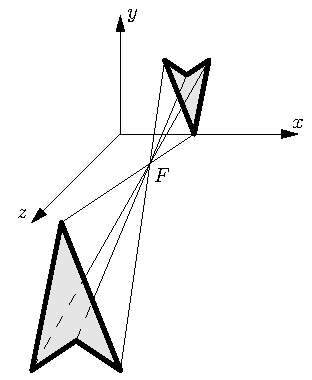
\includegraphics{figures/fig1_8_1.pdf}
    \caption{到$x$-$y$平面上的透视投影：$F$是投影中心（焦点）}
    \label{fig_2}
\end{figure}

这就是照相机的工作原理，也是对我们眼球运作方式的合理且初步的近似。

\begin{figure}[htbp]
    \centering
    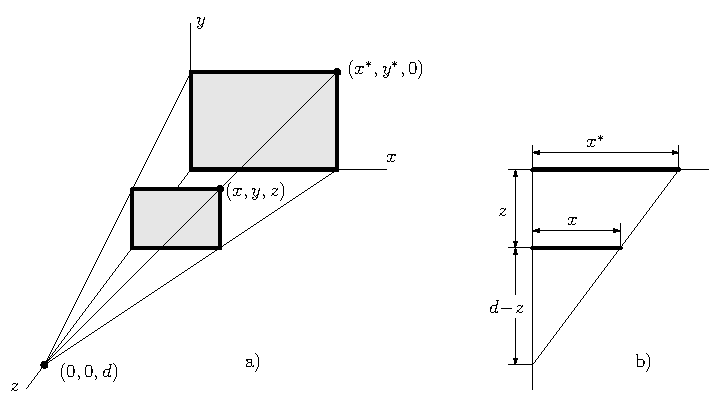
\includegraphics{figures/fig1_8_2.pdf}
    \caption{求出点$(x,y,z)^T$的透视投影的坐标$x^\ast,y^\ast$}
    \label{fig_3}
\end{figure}

下面推导这种投影的公式。假设焦点是$(0,0,d)^T$，并且是向$x$-$y$平面上投影——见图 \ref{fig_3} a)。考虑点$\mathbf{v}=(x,y,z)^T$，并令$\mathbf{v}^*=(x^*,y^*,0)^T$是其投影。如图 \ref{fig_3} b)，分析相似三角形可得\[\frac{x^*}{d}=\frac{x}{d-z},\]
故\[x^*=\frac{xd}{d-z}=\frac{x}{1-z/d},\]
类似有\[y^*=\frac{y}{1-z/d}.\]
注意，此公式同样适用于$z>d$和$z<0$的情况：你可以自行绘制对应的相似三角形来检验。

于是透视投影将点$(x,y,z)^T$映射到点$\begin{pmatrix}\frac{x}{1-z/d},\frac{y}{1-z/d},0\end{pmatrix}^T$。

该变换显然不是线性的（由于分母中的$z$）。然而，可以将它表示为线性变换。为此，我们引入所谓{\bf 齐次坐标}。

在齐次坐标中，$\mathbb{R}^3$中的每个点都用$4$个坐标来表示，其中最后一个（即第$4$个）坐标充当缩放系数的角色。从而，要从向量$\mathbf{v}$的齐次坐标$(x_1,x_2,x_3,x_4)^T$恢复出通常的$3$维坐标$(x,y,z)^T$，我们需要将每项都除以最后一个坐标$x_4$，再取前三个坐标\footnote{如果我们将$\mathbb{R}^3$中一个点的齐次坐标乘以一个非零标量，这个点不会改变。换言之，在齐次坐标中，$\mathbb{R}^3$中的点是用$\mathbb{R}^4$中过$\mathbf{0}$的直线来表示的。}（若$x_4=0$，那么此办法就不奏效了，因此我们假设$x_4=0$对应的是处于无穷远处的点）。

于是在齐次坐标中，向量$\mathbf{v}^{*}$可表示为$(x,y,0,1-z/d)^T$，因此在齐次坐标中，透视投影是线性变换：
\[\begin{pmatrix}x\\y\\0\\1-z/d\end{pmatrix}=\begin{pmatrix}1&0&0&0\\0&1&0&0\\0&0&0&0\\0&0&-1/d&1\end{pmatrix}\begin{pmatrix}x\\y\\z\\1\end{pmatrix}.\]
注意在齐次坐标中，平移也是线性变换：\[\begin{pmatrix}x+a_1\\y+a_2\\z+a_3\\1\end{pmatrix}=\begin{pmatrix}1&0&0&a_1\\0&1&0&a_2\\0&0&1&a_3\\0&0&0&1\end{pmatrix}\begin{pmatrix}x\\y\\z\\1\end{pmatrix}.\]

不过，如果投影中心不是$(0,0,d)^T$，而是任意的点$(d_1,d_2,d_3)^T$呢？那么，我们需要首先做平移量为$-(d_1,d_2,0)^T$的平移，将投影中心移到$(0,0,d_3)^T$（同时保持$x$-$y$平面不变），再作用该投影，然后再用平移量为$(d_1,d_2,0)^T$的平移来抵消之前的平移。类似地，如果投影平面不是$x$-$y$平面，就需要通过旋转和平移将投影平面转到$x$-$y$平面上，之后的逻辑类似上述过程。

所有这些运算都仅仅是与$4\times 4$矩阵的乘法。这就能够解释为何现代的显卡在处理器中内置了$4\times 4$矩阵运算。

当然，此处我们只是对$3$维图形学背后的数学有了粗浅的认识，还有许多可供了解的地方。例如，怎样确定一个物体的哪些部分是可见或不可见的，如何制造逼真的光影，等等。

\begin{problemset}
    \item $\mathbb{R}^3$中的哪个向量具有齐次坐标$(10,20,30,5)$？
    \item 证明：旋转$\gamma$可表示为以下这两个“剪切与缩放”变换的复合：
    \[T_1=\begin{pmatrix}1&0\\\sin\gamma&\cos\gamma\end{pmatrix},\quad T_2=\begin{pmatrix}\sec\gamma&-\tan\gamma\\0&1\end{pmatrix}.\]
    两变换的顺序应该是什么样？
    \item 将$2$维向量乘以任意$2\times 2$矩阵通常需要做$4$次乘法。
    
    假设$2\times 1000$矩阵$D$包含$\mathbb{R}^2$中的$1000$个点。利用两个任意的$2\times 2$矩阵来变换这些点，需要做多少次乘法？请比较两种可能的算法，$A(BD)$和$(AB)D$。
    \item 写出表征投影中心为$(d_1,d_2,d_3)^T$、投影平面为$x$-$y$平面的透视投影的矩阵。
    \item $\mathbb{R}^3$中的变换$T$将向量绕$x$-$y$平面中的直线$y=x+3$旋转$\gamma$。写出对应于该变换的$4\times 4$矩阵。
    
    你可将答案保留为若干矩阵相乘的形式。
\end{problemset}

%----- 第2章 线性方程组 -----

%%%%%%%%%%%%%%%%% 线性方程组 %%%%%%%%%%%%%%

\chapter{线性方程组}\label{chap:LinearSystems}

\section{线性方程组的多副面孔}

关于线性方程组为何物，有多种视角。第一种（也是最朴素的一种），就是将其视作含有$n$个未知数$x_1,x_2,\dots,x_n$的$m$个线性方程，
\[\left\{\begin{array}{cccccccccc}a_{1,1}x_1&+&a_{1,2}x_2&+&\ldots&+&a_{1,n}x_n&=&b_1\\a_{2,1}x_1&+&a_{2,2}x_2&+&\ldots&+&a_{2,n}x_n&=&b_2\\\cdots\\a_{m,1}x_1&+&a_{m,2}x_2&+&\ldots&+&a_{m,n}x_n&=&b_m&.\end{array}\right.\]

求解该方程组即求出{\bf 所有}同时满足这$m$个方程的数$x_1,x_2,\dots,x_n$构成的$n$-元组。

如果记$\mathbf{x}:=(x_{1},x_{2},\ldots,x_{n})^{T}\in\mathbb{F}^{n},\mathbf{b}=(b_{1},b_{2},\ldots,b_{m})^{T}\in\mathbb{F}^{m}$，且记
\[A=\begin{pmatrix}a_{1,1}&a_{1,2}&\ldots&a_{1,n}\\a_{2,1}&a_{2,2}&\ldots&a_{2,n}\\\vdots&\vdots&&\vdots\\a_{m,1}&a_{m,2}&\ldots&a_{m,n}\end{pmatrix},\]
那么上述线性方程组可以写成{\bf 矩阵形式}（也即{\bf 矩阵-向量方程}）
\[A\mathbf{x}=\mathbf{b}.\]
求解上述方程即求出所有满足$A\mathbf{x}=\mathbf{b}$的向量$\mathbf{x}\in\mathbb{F}^{n}$。

最后，回想一下矩阵-向量乘法的“列乘以坐标”规则，我们可以将原方程组写为{\bf 向量方程}
\[x_1\mathbf{a}_1+x_2\mathbf{a}_2+\cdots+x_n\mathbf{a}_n=\mathbf{b},\]
其中$\mathbf{a}_k$是矩阵$A$的第$k$列，$\mathbf{a}_k=(a_{1,k},a_{2,k},\dots,a_{m,k})^T,k=1,2,\dots,n$。

注意，上面三例本质上只是同种数学对象的不同表达而已。

在开始解释如何求解线性方程组之前，我们首先要注意，未知数的记法——比如$x_k,y_k$或者其他名称——都无关紧要。所以，求解线性方程组所必需的信息全部包含于两者：矩阵$A$（称为线性方程组的{\bf 系数矩阵}）和（右端）向量$\mathbf{b}$。进而，我们所需的全部信息都包含于以下矩阵
\pagebreak
\[\left(
  \begin{array}{cccc|c}
      a_{1,1} & a_{1,2} & \ldots & a_{1,n} & b_1    \\
      a_{2,1} & a_{2,2} & \ldots & a_{2,n} & b_2    \\
      \vdots  & \vdots  &        & \vdots  & \vdots \\
      a_{m,1} & a_{m,2} & \ldots & a_{m,n} & b_m    \\
    \end{array}
  \right)\]
该矩阵是通过将列向量$\mathbf{b}$增加到矩阵$A$右端获得的，称为线性方程组的{\bf 增广矩阵}。我们通常会在$A$和$\mathbf{b}$之间插入一条竖线来区分增广矩阵和系数矩阵。


\section{线性方程组的解、阶梯形和简化阶梯形}

线性方程组是用{\bf 高斯-若当消元法}（有时也称为{\bf 行化简}）来求解的。通过对线性方程组的增广矩阵的行作变换（也即对方程作变换），我们将其化为一简单的形式——即所谓{\bf 阶梯形}。当线性方程组具有{\bf 阶梯形}时，我们就很容易写出其解。

\subsection{行变换}

行变换有三种：
\begin{enumerate}
  \item 行交换：交换矩阵的两行；
  \item 缩放：将一行乘以非零标量$a$；
  \item 行置换：将第$k$行换为它与第$j$行的常数倍之和，而保持其他行不变。
\end{enumerate}

显然，变换1和2并不会改变线性方程组的解集——它们实质上就没有改变原方程组。

至于变换3，我们容易看出它不会使方程组的解减少。意即，令“新”方程组由“旧”方程组经过第3种行变换得来。那么“旧”方程组的每个解都是“新”方程组的解。

要看出为什么变换3不会导致解增加，也就是“新”方程组的任一解也是“旧”方程组的解，我们只需注意到第3种行变换是{\bf 可逆的}，也即，“旧”方程组也可以通过对“新”方程组进行第3种行变换得来（你能说出是什么样的变换吗？）

\subsubsection{行变换与乘以初等矩阵}

关于上述行变换为何不改变方程组的解集，还有一种更为“高级”的解释，也即，每种行变换都等价于左乘一种特殊的初等矩阵。

\setcounter{MaxMatrixCols}{12}
具体地说，乘以矩阵
\[
\begin{pNiceMatrix}[margin,first-row,first-col]
    &        &        &        & j      &        &        &        & k      &                        &              & \\
    & 1      &        &        & \vdots &        &        &        & \vdots & \Block{3-3}<\LARGE>{0} &              & \\
    &        & \ddots &        & \vdots &        &        &        & \vdots &                        & \hspace{1em} & \\
    &        &        & 1      & \vdots &        &        &        & \vdots &                        &              & \\
  j & \cdots & \cdots & \cdots & 0      & \cdots & \cdots & \cdots & 1      &                        &              & \\
    &        &        &        & \vdots & 1      &        &        & \vdots &                        &              & \\
    &        &        &        & \vdots &        & \ddots &        & \vdots &                        &              & \\
    &        &        &        & \vdots &        &        & 1      & \vdots &                        &              & \\
  k & \cdots & \cdots & \cdots & 1      & \cdots & \cdots & \cdots & 0      &                        &              & \\
    &        & \Block{3-2}<\LARGE>{0} &        &        &       &        &        &  &            1            &              & \\
    &        & \hspace{1em} &        &        &       &        &        &  &                        &        \ddots      & \\
    &        &  &        &        &       &        &        &  &                        &              & 1 
\end{pNiceMatrix}
\]
即交换第$j$行与第$k$行；乘以矩阵
\[
\begin{pNiceMatrix}[margin,first-col,first-row]
    &                        &        &   &   k    &   &                        &   \\
    & 1                      &        &   & \vdots &   & \Block{3-2}<\LARGE>{0} &   \\
    &                        & \ddots &   & \vdots &   &                        &   \\
    &                        &        & 1 & 0      &   &                        &   \\
  k & \cdots                 & \cdots & 0 & a      & 0 &                        &   \\
    & \Block{3-2}<\LARGE>{0} &        &   & 0      & 1 &                        &   \\
    &                        &        &   &        &   & \ddots                 & 0 \\
    &                        &        &   &        &   & 0                      & 1 \\
\end{pNiceMatrix}
\]
即将第$k$行乘以$a$。最后，乘以矩阵
\[
\begin{pNiceMatrix}[margin,first-row,first-col]
    &                        &        & j      &        & k      &                        &   \\
    & 1                      &        & \vdots &        & \vdots & \Block{2-2}<\LARGE>{0} &   \\
    &                        & \ddots & \vdots &        & \vdots &                        &   \\
  j & \cdots                 & \cdots & 1      & \cdots & 0      &                        &   \\
    &                        &        & \vdots & \ddots & \vdots &                        &   \\
  k & \cdots                 & \cdots & a      & \cdots & 1      &                        &   \\
    & \Block{2-2}<\LARGE>{0} &        &        &        &        & \ddots                 &   \\
    &                        &        &        &        &        &                        & 1
\end{pNiceMatrix}
\]
即将第$k$行加上第$j$行的$a$倍，并保持其他行不变。

要看出与这些矩阵相乘能实现上述效果，\marginpar{\small 一种描述（或记忆）这些初等矩阵的方式是：它们是向$I$施加对应行变换的结果。}只需要观察列向量乘以这些矩阵会发生什么变化。

注意所有初等矩阵都可逆（这对应于行变换的可逆性）。第一个矩阵的逆就是其本身。要得到第二个矩阵的逆，只需将$a$换成$1/a$。最后，通过将$a$换成$-a$可得第三个矩阵的逆。这些逆的正确性同样可通过观察列向量乘以这些矩阵会发生何种变化来检验。

因此，对方程组$A\mathbf{x}=\mathbf{b}$的增广矩阵作行变换等价于向该方程组左端乘上一个特殊的可逆矩阵$E$。在等式$A\mathbf{x}=\mathbf{b}$两端左乘$E$可得，方程\[A\mathbf{x}=\mathbf{b}\]的任意解也是方程\[EA\mathbf{x}=E\mathbf{b}\]的解。将这个方程左乘$E^{-1}$可得，其任意解是下述方程\[E^{-1}EA\mathbf{x}=E^{-1}E\mathbf{b}\]的解，也就是原方程$A\mathbf{x}=\mathbf{b}$的解。因此，行变换不改变方程组的解集。

\subsection{行化简}

行化简的主要步骤包含下面三步：
\begin{enumerate}
  \item 找到矩阵最左侧的非零列；
  \item 如有必要，通过施加第一类行变换（行交换），确保该列的第一个（最上方的）项是非零的。该项将被称为{\bf 主元}；
  \item 通过向第$2,3,\dots,m$行加（或减）第一行的适当倍数，“消去”主元之下的所有非零项（就是将它们都变为$0$）。
\end{enumerate}
我们先将这些步骤作用于整个矩阵，然后保持第一行不变并将这些步骤作用于第$2,3,\dots,m$行，然后是第$3,\dots,m$行，以此类推。

关键是记住在把某一行下方的所有行都减去该行的若干倍后（步骤3），我们就不再改变该行（甚至不会将该行与其他行进行交换）。

在有限次（至多$m$次）应用这些步骤后，我们就得到了矩阵的{\bf 阶梯形}。

\subsubsection{行化简实例}

考虑如下线性方程组：\[\left\{\begin{array}{c}x_1+2x_2+3x_3=1\\3x_1+2x_2+x_3=7\\2x_1+x_2+2x_3=1\end{array}\right.\]
该方程组的增广矩阵是
\[\left(
  \begin{array}{ccc|c}
      1 & 2 & 3 & 1   \\
      3 & 2 & 1 & 7   \\
      2 & 1 & 2 & 1   \\
    \end{array}
  \right)\]
将第二行减去第一行的$3$倍，并将第三行减去第一行的$2$倍，我们得到：
\[\begin{pNiceArray}{ccc|c}[margin,last-col]
  1 & 2 & 3 & 1 &  \\
  3 & 2 & 1 & 7 & -3R_1  \\
  2 & 1 & 2 & 1 & -2R_1 \\
\end{pNiceArray} \quad\sim\quad \left(
  \begin{array}{rrr|r}
      1 & 2 & 3 & 1   \\
      0 & -4 & -8 & 4   \\
      0 & -3 & -4 & -1   \\
    \end{array}
  \right)
\]
将第二行乘以$-1/4$可得
\[\left(
  \begin{array}{rrr|r}
    1 & 2 & 3 & 1   \\
    0 & 1 & 2 & -1   \\
    0 & -3 & -4 & -1   \\
  \end{array}
\right)\]
将第二行的$3$倍加到第三行，可得
\[\begin{pNiceArray}{rrr|r}[margin,last-col]
  1 & 2 & 3 & 1 &  \\
  0 & 1 & 2 & -1 &   \\
  0 & -3 & -4 & -1 & +3R_2 \\
\end{pNiceArray} \quad\sim\quad \left(
  \begin{array}{rrr|r}
      1 & 2 & 3 & 1   \\
      0 & 1 & 2 & -1   \\
      0 & 0 & 2 & -4   \\
    \end{array}
  \right)
\]
现在，我们就可用所谓{\bf 回代法}解此方程组了。也就是说，从最后一行（最后一个方程）得出$x_3 = -2$。接下来从第二个方程得到\[x_2=-1-2x_3=-1-2(-2)=3,\]
最后从第一行（第一个方程）得到\[x_1=1-2x_2-3x_3=1-6+6=1.\]
因此原方程组的解为\[\left\{\begin{array}{l}x_1=1,\\x_2=3,\\x_3=-2,\end{array}\right.\]
或用向量形式表示为\[\mathbf{x}=\begin{pmatrix}1\\3\\-2\end{pmatrix}\]
或写为$\mathbf{x}=(1,3,-2)^T$。我们可以通过作乘法$A\mathbf{x}$来检验该解，其中$A$为系数矩阵。

我们也可以不用回代法，而是从下到上做行变换，将系数矩阵主对角线上方的所有项全部变为$0$：首先将最后一行乘以$1/2$，后续过程则不言而喻：
\begin{align*}
  \begin{pNiceArray}{rrr|r}[margin,last-col]
    1 & 2 & 3 & 1 & -3R_3 \\
    0 & 1 & 2 & -1 &  -2R_3 \\
    0 & 0 & 1 & -2 &  \\
  \end{pNiceArray} &\sim 
  \begin{pNiceArray}{rrr|r}[margin,last-col]
        1 & 2 & 0 & 7 & -2R_2 \\
        0 & 1 & 0 & 3   \\
        0 & 0 & 1 & -2   \\
  \end{pNiceArray}\\
  &\sim\begin{pNiceArray}{rrr|r}[margin]
    1 & 0 & 0 & 1 \\
    0 & 1 & 0 & 3   \\
    0 & 0 & 1 & -2   \\
\end{pNiceArray}
\end{align*}
然后从增广矩阵一眼可知解为$\mathbf{x}=(1,3,-2)^T$。

留给读者一道习题：梳理从下到上阶段的行化简算法。

\subsection{阶梯形}\label{subsec:echelon}

矩阵具有{\bf 阶梯形}，若其满足如下两个条件：
\begin{enumerate}
  \item 所有的零行（即全部的项都等于$0$的行）位于所有非零项的下方；
\end{enumerate}
对于非零行，我们称最左边的非零项为{\bf 先导元}。那么阶梯形的第二个性质可表述为：
\begin{enumerate}[start=2]
  \item 任意非零行的先导元必定严格处于前一行先导元的右侧。
\end{enumerate}

阶梯形中每一行的先导元也称为{\bf 主元}，\marginpar{\small 主元：一行中的先导元（最左侧的非零项）。}因为这些项恰为行化简时所用的{\bf 主元}。

阶梯形有个特例是所谓{\bf 三角}形。在上面的例子中我们就得到了这种形式。在这种形式中，系数矩阵是方阵（$n\times n$矩阵），其主对角线项均不为零，而主对角线之下的所有项都为零。右端项，或者说增广矩阵的最右列可以是任意的。

在行化简的从下到上阶段之后，我们就得到了矩阵的所谓{\bf 简化阶梯形}：系数矩阵等于$I$（如上例所示）是简化阶梯形的一个特例。

一般的定义是：称矩阵具有{\bf 简化阶梯形}，若其具有阶梯形且
\begin{enumerate}[start=3]
  \item 所有主元都等于$1$；
  \item 主元之上的所有项都为$0$。注意，主元之下的所有项也都是$0$，因为该矩阵具有阶梯形。
\end{enumerate}

为了从阶梯形得到简化阶梯形，我们按从下到上、从右到左的次序，利用行置换消去主元之上的所有项。

简化阶梯形的一个例子是系数矩阵等于$I$的方程组。在这种情况下，从简化阶梯形就很容易看出解。在一般的情形下，从简化阶梯形看出解也很容易。例如，令方程组（增广矩阵）的简化阶梯形是\[\left(\begin{array}{ccccc|c}\boxed{1}&2&0&0&0&1\\0&0&\boxed{1}&5&0&2\\0&0&0&0&\boxed{1}&3\end{array}\right);\]
此处我们将主元框出来了。求解思路是，将没有主元的列所对应的变量（所谓{\bf 自由变量}）移到右侧。然后我们可直接写出解为\pagebreak\[\left\{\begin{array}{l}x_1=1-2x_2\\x_2~\text{为自由变量}\\x_3=2-5x_4\\x_4~\text{为自由变量}\\x_5=3\end{array}\right.\]
或者写成向量形式
\[\mathbf{x}=\begin{pmatrix}1-2x_2\\x_2\\2-5x_4\\x_4\\3\end{pmatrix}=\begin{pmatrix}1\\0\\2\\0\\3\end{pmatrix}+x_2\begin{pmatrix}-2\\1\\0\\0\\0\end{pmatrix}+x_4\begin{pmatrix}0\\0\\-5\\1\\0\end{pmatrix},\quad x_2,x_4\in\mathbb{F}.\]

也可用回代法从阶梯形求出解：基本思路是从下到上操作，将所有自由变量移到右侧。
\begin{problemset}
  \item 将下列线性方程组写成矩阵形式和向量方程形式：
  \begin{enumerate}[label={\alph*)}]
    \item $\left\{\begin{array}{rrrrrrrr}x_1&+&2x_2&-&x_3&=&-1\\2x_1&+&2x_2&+&x_3&=&1\\3x_1&+&5x_2&-&2x_3&=&-1\end{array}\right.$
    \item $\left\{\begin{array}{rrrrrrrr}x_1&-&2x_2&-&x_3&=&1\\2x_1&-&3x_2&+&x_3&=&6\\3x_1&-&5x_2&&&=&7\\x_1&&&+&5x_3&=&9\end{array}\right.$
    \item $\left\{\begin{array}{rrrrrrrrrr}x_1&+&2x_2&&&+&2x_4&=&6\\3x_1&+&5x_2&-&x_3&+&6x_4&=&17\\2x_1&+&4x_2&+&x_3&+&2x_4&=&12\\2x_1&&&-&7x_3&+&11x_4&=&7\end{array}\right.$
    \item $\left\{\begin{array}{rrrrrrrrrr}x_1&-&4x_2&-&x_3&+&x_4&=&3\\2x_1&-&8x_2&+&x_3&-&4x_4&=&9\\-x_1&+&4x_2&-&2x_3&+&5x_4&=&-6\end{array}\right.$
    \item $\left\{\begin{array}{rrrrrrrrrr}x_1&+&2x_2&-&x_3&+&3x_4&=&2\\2x_1&+&4x_2&-&x_3&+&6x_4&=&5\\&&x_2&&&+&2x_4&=&3\end{array}\right.$
    \item $\left\{\begin{array}{rrrrrrrrrrr}2x_1&-&2x_2&-&x_3&+&6x_4&-&2x_5&=&1\\x_1&-&x_2&+&x_3&+&2x_4&-&x_5&=&2\\4x_1&-&4x_2&+&5x_3&+&7x_4&-&x_5&=&6\end{array}\right.$
    \item $\left\{\begin{array}{rrrrrrrrrrrr}3x_1&-&x_2&+&x_3&-&x_4&+&2x_5&=&5\\x_1&-&x_2&-&x_3&-&2x_4&-&x_5&=&2\\5x_1&-&2x_2&+&x_3&-&3x_4&+&3x_5&=&10\\2x_1&-&x_2&&&-&2x_4&+&x_5&=&5\end{array}\right.$
  \end{enumerate}
  解这些方程组。将解写成向量形式。
  \item 求出向量方程\[x_1\mathbf{v}_1+x_2\mathbf{v}_2+x_3\mathbf{v}_3=\mathbf{0},\]的{\bf 全部}解，其中$\mathbf{v}_{1}=(1,1,0)^{T},\mathbf{v}_{2}=(0,1,1)^{T},\mathbf{v}_{3}=(1,0,1)^{T}$。关于向量组$\mathbf{v}_1,\mathbf{v}_2,\mathbf{v}_3$的线性无关性（线性相关性），你可以得出什么结论？
\end{problemset}

\section{主元分析}

通过分析线性方程组增广矩阵的阶梯形（简化阶梯形）的主元，可以回答所有关于解的存在性和唯一性的问题。首先要分析的问题是：方程$A\mathbf{x}=\mathbf{b}$何时会{\bf 不相容}（无解）。稍加思索可立得答案：
\begin{center}
  \fbox{\parbox{0.8\linewidth}{方程组不相容（无解），当且仅当{\bf 增广}矩阵的阶梯形的最后一列存在主元，也就是，当且仅当增广矩阵的阶梯形有一行是$\left(\begin{array}{cccc|c}0&0&\ldots&0&b\end{array}\right),b\neq0$。}}
\end{center}
的确如此：这样一行对应于方程$0x_1+0x_2+\ldots+0x_n=b\neq0$，而该方程无解。如果不存在这样的行，我们就可以将增广矩阵化为简化阶梯形并直接看出方程组的解。

下面再列出三个结论。注意，它们是与方程组的{\bf 系数矩阵}而非增广矩阵相关。
\begin{enumerate}
  \item 方程组的解（若存在）是唯一的，当且仅当没有自由变量，也就是当且仅当系数矩阵的阶梯形在每一列中都有主元；
  \item 方程$A\mathbf{x}=\mathbf{b}$对于任意右端项$\mathbf{b}$都是相容的，当且仅当系数矩阵的阶梯形在每一行中都有主元；
  \item 方程$A\mathbf{x}=\mathbf{b}$对于任意右端项$\mathbf{b}$都有{\bf 唯一解}，当且仅当系数矩阵$A$的阶梯形在每一行和每一列中都有主元。
\end{enumerate}

第一个结论很平凡，因为自由变量对应于非唯一性。只是要强调，这一结论{\bf 并不保证}存在性。

第二个结论稍复杂些。若系数矩阵的每行都有主元，{\bf 增广}矩阵的最后一列就不会有主元，因此无论右端项$\mathbf{b}$是什么，方程组都是相容的。

下面证明，如果系数矩阵$A$的阶梯形中有零行，那么可以选择一个右端项$\mathbf{b}$使得方程组$A\mathbf{x}=\mathbf{b}$是不相容的。令$A_{\mathrm{e}}$为系数矩阵$A$的阶梯形。那么\[A_{\mathrm{e}}=EA\]其中$E$是一系列初等矩阵之积，对应于一系列行变换，$E=E_N\dots E_2E_1$。若$A_{\mathrm{e}}$有零行，那么其最后一行也为零。因此，如果取$\mathbf{b}_\mathrm{e}=(0,\ldots,0,1)^T$（除了最后一项以外各项全为$0$）那么方程\[A_{\mathrm{e}}\mathbf{x}=\mathbf{b}_e\]无解。方程两端同时左乘$E^{-1}$，并运用$E^{-1}A_{\mathrm{e}}=A$，可得方程\[A\mathbf{x}=E^{-1}\mathbf{b}_\mathrm{e}\]
无解。

最后，由结论1和2可立得结论3。{\hfill\qedsymbol}

从以上对于主元的分析可得若干重要推论。为此我们需要注意到
\begin{center}
  \fbox{\parbox{0.8\linewidth}{在阶梯形中，任一行和任一列中至多存在一个主元（可以没有主元）。}}
\end{center}

\subsection{有关线性无关性和基的推论、维数}

通过行化简，很容易回答$\mathbb{F}^n$中的向量组何时为基、线性无关组或张成组的问题。

\begin{proposition}\label{prop:li_span_eq}
  设有向量组$\mathbf{v}_{1},\mathbf{v}_{2},\ldots,\mathbf{v}_{m}\in\mathbb{F}^{n}$，并令$A=[\mathbf{v}_{1},\mathbf{v}_{2},\ldots,\mathbf{v}_{m}]$是各列为$\mathbf{v}_{1},\mathbf{v}_{2},\ldots,\mathbf{v}_{m}$的$n\times m$矩阵。那么
  \begin{enumerate}
    \item 向量组$\mathbf{v}_{1},\mathbf{v}_{2},\ldots,\mathbf{v}_{m}$是线性无关的，当且仅当$A$的阶梯形的每一列都有主元；
    \item 向量组$\mathbf{v}_{1},\mathbf{v}_{2},\ldots,\mathbf{v}_{m}$是$\mathbb{F}^{n}$中的完备组（张成组、生成组），当且仅当$A$的阶梯形的每一行都有主元；
    \item 向量组$\mathbf{v}_{1},\mathbf{v}_{2},\ldots,\mathbf{v}_{m}$是$\mathbb{F}^{n}$中的基，当且仅当$A$的阶梯形的每一行与每一列都有主元。
  \end{enumerate}
\end{proposition}
\begin{proof}
  向量组$\mathbf{v}_{1},\mathbf{v}_{2},\ldots,\mathbf{v}_{m}\in\mathbb{F}^{n}$线性无关，当且仅当方程\[x_1\mathbf{v}_1+x_2\mathbf{v}_2+\ldots+x_m\mathbf{v}_m=\mathbf{0}\]具有唯一（平凡）解$x_{1}=x_{2}=\ldots=x_{m}=0$，或等价于，方程$A\mathbf{x}=\mathbf{0}$具有唯一解$\mathbf{x}=\mathbf{0}$。根据前述结论1，这些等价于矩阵的阶梯形每一列都有主元。

  类似地，向量组$\mathbf{v}_{1},\mathbf{v}_{2},\ldots,\mathbf{v}_{m}\in\mathbb{F}^{n}$是$\mathbb{F}^{n}$中的完备组，当且仅当方程\[x_1\mathbf{v}_1+x_2\mathbf{v}_2+\cdots+x_m\mathbf{v}_m=\mathbf{b}\]对任意右端项$\mathbf{b}\in\mathbb{F}^n$都有解。根据前述结论2，这等价于矩阵的阶梯形的每一行都有主元。

  最后，向量组$\mathbf{v}_{1},\mathbf{v}_{2},\ldots,\mathbf{v}_{m}\in\mathbb{F}^{n}$是$\mathbb{F}^{n}$中的基，当且仅当方程\[x_1\mathbf{v}_1+x_2\mathbf{v}_2+\cdots+x_m\mathbf{v}_m=\mathbf{b}\]对任意右端项$\mathbf{b}\in\mathbb{F}^n$都有唯一解。根据前述结论3，这等价于$A$的阶梯形的每一行和每一列都有主元。
\end{proof}

\begin{proposition}\label{prop:li_no_more}
  $\mathbb{F}^{n}$中的任意线性无关向量组不能含有超过$n$个向量。
\end{proposition}

\begin{proof}
  设向量组$\mathbf{v}_{1},\mathbf{v}_{2},\ldots,\mathbf{v}_{m}\in\mathbb{F}^{n}$线性无关，并令$A=[\mathbf{v}_{1},\mathbf{v}_{2},\ldots,\mathbf{v}_{m}]$是各列为$\mathbf{v}_{1},\mathbf{v}_{2},\ldots,\mathbf{v}_{m}$的$n\times m$矩阵。由命题 \ref{prop:li_span_eq}，$A$的阶梯形的每列都必有主元，而这在$m>n$时是不可能的（主元的数目不会超过行数）。
\end{proof}

\begin{proposition}\label{prop:basis_same_size}
  向量空间$V$中的任意两个基都有相同个数的向量。
\end{proposition}

\begin{proof}
  设$\mathbf{v}_{1},\mathbf{v}_{2},\ldots,\mathbf{v}_{n}$和$\mathbf{w}_{1},\mathbf{w}_{2},\ldots,\mathbf{w}_{m}$是$V$中两个不同的基。不失一般性，可假设$n\le m$。考虑定义如下的同构$A:\mathbb{F}^{n}\to V$：\[A\mathbf{e}_k=\mathbf{v}_k,\quad k=1,2,\ldots n,\]其中$\mathbf{e}_1,\mathbf{e}_2,\ldots,\mathbf{e}_n$是$\mathbb{R}^n$中的标准基。

  由于$A^{-1}$也是同构，因此向量组\[A^{-1}\mathbf{w}_1,A^{-1}\mathbf{w}_2,\ldots,A^{-1}\mathbf{w}_m\]也是基（见第 \ref{chap:BasicNotion} 章的\autoref{thm:preserve_basis}）。因此它是线性无关的，则由命题 \ref{prop:li_no_more} 可知$m\le n$。结合$n\le m$的假设即得$m=n$。
\end{proof}

接下来的结论是上述命题的一个特殊情况。
\begin{proposition}\label{prop:basis_size_n}
    $\mathbb{F}^{n}$中的任意一个基都恰有$n$个向量。
\end{proposition}
\begin{proof}
  从上个命题可立即得到此结论，不过也可以直接证明。设$\mathbf{v}_{1},$ $\mathbf{v}_{2},\ldots,\mathbf{v}_{m}$是$\mathbb{F}^{n}$中的基，并令$A$是各列为$\mathbf{v}_{1},\mathbf{v}_{2},\ldots,\mathbf{v}_{m}$的$n\times m$矩阵。该向量组是基，意味着方程\[A\mathbf{x}=\mathbf{b}\]对任意（所有可能的）右端项$\mathbf{b}$都有唯一解。解的存在性表明该矩阵的简化阶梯形每行都有主元，因此主元的数目恰为$n$，唯一性则表明系数矩阵（的阶梯形）每列都有主元。因此\[m = \text{列数} = \text{主元数} = n\]
\end{proof}

\begin{proposition}\label{prop:span_more}
  $\mathbb{F}^{n}$中的任意张成（生成）组都至少包含$n$个向量。
\end{proposition}
\begin{proof}
  设$\mathbf{v}_{1},$ $\mathbf{v}_{2},\ldots,\mathbf{v}_{m}$是$\mathbb{F}^{n}$中的完备组，并令$A$是各列为$\mathbf{v}_{1},\mathbf{v}_{2},\ldots,$ $\mathbf{v}_{m}$的$n\times m$矩阵。命题 \ref{prop:li_span_eq} 的结论2表明，$A$的阶梯形的每行都有主元。因为主元数目不超过列数，所以$n\le m$。
\end{proof}

\subsection{有关可逆矩阵的推论}

\begin{proposition}
  矩阵$A$可逆，当且仅当其阶梯形的每一行和每一列都有主元。
\end{proposition}

\begin{proof}
  我们在本节开头已讨论过，方程$A\mathbf{x}=\mathbf{b}$对于任意右端项$\mathbf{b}$都有唯一解，当且仅当$A$的阶梯形在每一行和每一列中都有主元。又由第 \ref{chap:BasicNotion} 章定理 \ref{thm:invert_unique} 知，矩阵（线性变换）$A$是可逆的，当且仅当方程$A\mathbf{x}=\mathbf{b}$对于任意右端项$\mathbf{b}$都有唯一解。

  还有另一种证法：我们知道矩阵可逆当且仅当它的各列形成一个基（见第 \ref{chap:BasicNotion} 章 \ref{subsec:invert_eq} 小节的推论 \ref{col:invert_basis}）。而上述命题 \ref{prop:basis_size_n} 表明这等价于矩阵的阶梯形每一行和每一列都有主元。
\end{proof}

由上述命题立得下述结论：
\begin{corollary}
  可逆矩阵必为方阵（$n\times n$矩阵）。
\end{corollary}
\begin{proposition}
  若方阵（$n\times n$矩阵）是左可逆的或右可逆的，那么它是可逆的。换言之，为检验方阵$A$的可逆性，只需检验$AA^{-1}=I$, $A^{-1}A=I$之一。
\end{proposition}

注意，此命题只适用于方阵！

\begin{proof}
  我们知道矩阵$A$可逆当且仅当方程$A\mathbf{x}=\mathbf{b}$对于任意右端项$\mathbf{b}$都有唯一解。而这又等价于矩阵$A$的阶梯形在每一行和每一列中都有主元。

  若矩阵$A$是左可逆的，那么方程$A\mathbf{x}=\mathbf{0}$有唯一解$\mathbf{x}=\mathbf{0}$。的确如此：若$B$是$A$的左逆（也即$BA=I$），而$\mathbf{x}$满足\[A\mathbf{x}=\mathbf{0},\]
  那么将此等式两端同时左乘$B$，即得到$\mathbf{x}=\mathbf{0}$，则此解唯一。因此，$A$的阶梯形在每列中都有主元（无自由变量）。若矩阵$A$是方阵（$n\times n$矩阵），那么其阶梯形的每行也必有主元（共$n$个主元，而且每行至多有$1$个主元），因此该矩阵是可逆的。

  若矩阵$A$是右可逆的，且$C$是$A$的右逆（$AC=I$），那么对于$\mathbf{x}=C\mathbf{b},\mathbf{b}\in\mathbb{F}^{n}$，有\[A\mathbf{x}=AC\mathbf{b}=I\mathbf{b}=\mathbf{b}.\]
  因此，对任意右端项$\mathbf{b}$，方程$A\mathbf{x}=\mathbf{b}$都有解$\mathbf{x}=C\mathbf{b}$。于是$A$的阶梯形每一行都有主元。若$A$是方阵，那么它的每一列也都有主元，故$A$可逆。
\end{proof}

\begin{problemset}
  \item $b$取何值时，方程组\[\begin{pmatrix}1&2&2\\2&4&6\\1&2&3\end{pmatrix}\mathbf{x}=\begin{pmatrix}1\\4\\b\end{pmatrix}\]有解？对于该$b$，求方程组的通解。
  \item 判断向量组\[\begin{pmatrix}1\\1\\0\\0\end{pmatrix},\quad\begin{pmatrix}1\\0\\1\\0\end{pmatrix},\quad\begin{pmatrix}0\\0\\1\\1\end{pmatrix},\quad\begin{pmatrix}0\\1\\0\\1\end{pmatrix}\]是否为线性无关的。
  
  这四个向量能张成$\RR^4$吗？（换言之，它是生成组吗？）$\CC^4$呢？
  \item 判断下面哪些向量组是$\RR^3$中的基？
  \begin{enumerate}[label={\alph*)}]
    \item $(1,2,-1)^{T},(1,0,2)^{T},(2,1,1)^{T}$；
    \item $(-1,3,2)^{T},(-3,1,3)^{T},(2,10,2)^{T}$；
    \item $(67,13,-47)^{T},(\pi,-7.84,0)^{T},(3,0,0)^{T}$。
  \end{enumerate}
  哪些向量组是$\CC^3$的基？
  \item 多项式$x^{3}+2x,x^{2}+x+1,x^{3}+5$能否生成（张成）$\mathbb{P}_3$？证明你的结论。
  \item $\mathbb{F}^4$中的$5$个向量是否线性无关？证明你的结论。
  \item 证明或证伪：若方阵（$n\times n$矩阵）$A$的列是线性无关的，那么$A^2=AA$的列也是。
  \item 证明或证伪：若方阵（$n\times n$矩阵）$A$的列是线性无关的，那么$A^3=AAA$的列也是。
  \item 证明：如果方程$A\mathbf{x}=\mathbf{0}$有唯一解（即$A$的阶梯形每一列都有主元），那么$A$是左可逆的。
  
  {\bf 提示}：初等矩阵可能有用处。
  
  {\bf 注意}：正文中已经证明，若$A$是左可逆的则方程$A\mathbf{x}=\mathbf{0}$具有唯一解。此处你需要证明的是该结论的逆命题，而正文中并未给出证明。

  {\bf 注}：这题可能很难，因为它需要对所论述的主题有深刻的理解。然而，当理解需要做些什么之后，这道题就非常简单了。
  \pagebreak
  \item 矩阵的简化阶梯形是唯一的吗？证明你的结论。
  
  即，假设我们通过作任意行变换（不按照特定的算法）得到简化阶梯形矩阵。究竟是每次都会得到相同的矩阵，还是可能得到不同的矩阵？注意，只能作行变换，不允许做列变换。

  {\bf 提示}：如果你是从可逆矩阵开始做变换呢？另外，主元是始终在同样的列中，还是根据所做的行变换不同而处于不同的列？如果你可以不通过（对简化阶梯形）作相反的行变换来推知主元列的位置，那么主元列的位置就不取决于行变换。
\end{problemset}

\section{通过行化简求\texorpdfstring{$A^{-1}$}{A**\{-1\}}}

如上面所讨论的，可逆矩阵必为方阵，并且其阶梯形必定在每一行和每一列中都有主元。所以可逆矩阵的简化阶梯形是恒等矩阵$I$。因此
\begin{center}
  \fbox{\parbox{0.8\linewidth}{任意可逆矩阵都行等价于（即可通过行变换化为）恒等矩阵。}}
\end{center}

下面陈述一个用于求出$n\times n$矩阵的逆的简便算法：
\begin{enumerate}
  \item 向$A$的右侧附上$n\times n$恒等矩阵，将其{\bf 扩充}成$n\times 2n$的矩阵$(A|I)$；
  \item 对扩充后的矩阵作行变换，将$A$变换为恒等矩阵$I$；
  \item 我们添加的矩阵$I$在此过程中自动转化为$A^{-1}$；
  \item 如果通过行变换不能把$A$变换为恒等矩阵，那么$A$不可逆。
\end{enumerate}

上述算法有好几种解释。第一种（也是比较朴素的一种）是：我们知道对于可逆矩阵$A$，向量$A^{-1}\mathbf{b}$是方程$A\mathbf{x}=\mathbf{b}$的解。所以为了求出$A^{-1}$的第$k$列，我们需要求出$A\mathbf{x}=\mathbf{e}_k$的解，其中$\mathbf{e}_1,\mathbf{e}_2,\ldots,\mathbf{e}_n$是$\mathbb{R}^n$中的标准基。上述算法就是同时求解了如下$n$个方程\[A\mathbf{x}=\mathbf{e}_k,\quad k=1,2,\ldots,n\]

我们再展示一种更为“高级”的解释。之前我们讨论过，每次行变换都可通过左乘初等矩阵来实现。令$E_{1},E_{2},\ldots,E_{N}$是对应于我们所作的行变换的初等矩阵，并令$E=E_{N}\cdots E_{2}E_{1}$为它们的乘积\footnote{尽管此处顺序无关紧要，但请注意，若行变换$E_1$是最先进行的，那么在乘积中$E_1$是最右侧的一项。}。我们知道行变换可将$A$变为恒等矩阵，也即$EA=I$，故$E=A^{-1}$。同样的行变换作用于扩充的矩阵$(A|I)$，会将其变为$(EA|E) = (I|A^{-1})$。{\hfill \qedsymbol}

这种运用初等矩阵的“高级”解释蕴涵了之后会用到的一个重要命题：

\begin{theorem}\label{thm:invert_elementary_prod}
  任意可逆矩阵都可表示成若干初等矩阵之积。
\end{theorem}

\begin{proof}
  如前两段所讨论的，$A^{-1}=E_{N}\cdots E_{2}E_{1}$，所以\[A=(A^{-1})^{-1}=E_{1}^{-1}E_{2}^{-1}\cdots E_{N}^{-1}.\]
\end{proof}

\begin{example*}
  假设我们要求出以下矩阵的逆。
  \[\left(\begin{array}{rrr}1&4&-2\\-2&-7&7\\3&11&-6\end{array}\right).\]
  向其右侧附上恒等矩阵，并使用行变换可得
  \begin{align*}
  &\begin{pNiceArray}{rrr|rrr}[last-col]
    1&4&-2&1&0&0&\\
    -2&-7&7&0&1&0&+2R_1\\
    3&11&-6&0&0&1&-3R_1
  \end{pNiceArray}&&\sim 
  \begin{pNiceArray}{rrr|rrr}[last-col]
    1&4&-2&1&0&0&\\
    0&1&3&2&1&0&\\
    0&-1&0&-3&0&1&+R_2
  \end{pNiceArray}\sim\\
  &\begin{pNiceArray}{rrr|rrr}[last-col]
    1&4&-2&1&0&0&\times 3\\
    0&1&3&2&1&0&\\
    0&0&3&-1&1&1&
\end{pNiceArray}&&\sim 
  \begin{pNiceArray}{rrr|rrr}[last-col]
    3&12&-6&3&0&0&+2R_3\\
    0&1&3&2&1&0&-R_3\\
    0&0&3&-1&1&1&
  \end{pNiceArray}\sim
\end{align*}
在最后一次行变换中，我们将第一行乘以$3$倍是为了在行化简的从下到上阶段中不出现分数。
继续作行变换有
\begin{align*}
  \begin{pNiceArray}{rrr|rrr}[margin,last-col]
    3&12&0&1&2&2&-12R_2\\
    0&1&0&3&0&-1&\\
    0&0&3&-1&1&1&
  \end{pNiceArray}&\sim 
  \begin{pNiceArray}{rrr|rrr}[margin]
    3&0&0&-35&2&14\\
    0&1&0&3&0&-1\\
    0&0&3&-1&1&1
  \end{pNiceArray}
\end{align*}
将第一行和第三行除以$3$，就得到了逆矩阵\[\begin{pmatrix}-35/3&2/3&14/3\\3&0&-1\\-1/3&1/3&1/3\end{pmatrix}\]
\end{example*}

\begin{problemset}
  \item 求出下列矩阵的逆：
  \[\left(\begin{array}{ccc}1&2&1\\3&7&3\\2&3&4\end{array}\right),\quad\left(\begin{array}{ccc}1&-1&2\\1&1&-2\\1&1&4\end{array}\right).\]
  给出所有的步骤。
\end{problemset}

\section{维数、有限维向量空间}

\begin{definition*}
  向量空间$V$的维数$\dim V$是基所具有的向量个数。

  对于只包含零向量$\mathbf{0}$的向量空间，规定$\dim V=0$；若$V$不存在（有限的）基，则规定$\dim V=\infty$。

  若$\dim V$是有限值，则称$V$是{\bf 有限维的}；否则称其为{\bf 无限维的}。
\end{definition*}

命题 \ref{prop:basis_same_size} 确保了维数是定义完善的，也即，它并不依赖于基的选取。

第 \ref{chap:BasicNotion} 章的命题 \ref{prop:generating_contain_basis} 表明，向量空间$V$的任意有限张成组都包含一个基。由此立得
\begin{proposition}
  向量空间$V$是有限维的，当且仅当其包含有限张成组。
\end{proposition}

假设我们想检验有限维向量空间中的某向量组是否为基（或者检验其是否为线性无关的，或检验其是否完备）。最简单的方法大概是，利用同构$A:V\to \mathbb{R}^n,n=\dim V$将原问题转化到$\mathbb{R}^n$中，然后就可用行化简（分析主元）来回答这样的问题。

注意，若$\dim V=n$，那么同构$A:V\to \mathbb{R}^n$总是存在的。的确如此：若$\dim V=n$，那么存在基$\mathbf{v}_{1},\mathbf{v}_{2},\ldots,\mathbf{v}_{n}\in V$，于是可定义同构$A:V\to \mathbb{R}^n$为
\[A\mathbf{v}_k=\mathbf{e}_k,\quad k=1,2,\ldots,n.\]

下面给出命题 \ref{prop:li_no_more} 和 \ref{prop:span_more} 的两个推论，作为上述方法的示例。
\begin{proposition}\label{prop:arbit_li_no_more}
  有限维向量空间$V$中的任意线性无关组不会具有超过$\dim V$个向量。
\end{proposition}
\begin{proof}
  令$\mathbf{v}_1,\mathbf{v}_2,\ldots,\mathbf{v}_m\in V$为线性无关组，并令$A:V\to \mathbb{R}^n$为同构。那么$A\mathbf{v}_{1},A\mathbf{v}_{2},\ldots,A\mathbf{v}_{m}$是$\mathbb{R}^n$中的线性无关组，则由命题 \ref{prop:li_no_more} 知$m\le n$。
\end{proof}
\begin{proposition}\label{prop:arbit_span_more}
  有限维向量空间$V$中的任意生成组一定具有至少$\dim V$个向量。
\end{proposition}
\begin{proof}
  令$\mathbf{v}_1,\mathbf{v}_2,\ldots,\mathbf{v}_m\in V$为完备组，并令$A:V\to \mathbb{R}^n$为同构。那么$A\mathbf{v}_{1},A\mathbf{v}_{2},\ldots,A\mathbf{v}_{m}$是$\mathbb{R}^n$中的完备组，则由命题 \ref{prop:span_more} 知$m\ge n$。
\end{proof}

\subsection{将线性无关组补足为基}

下面结论将在后文发挥重要作用。

\begin{proposition}[补足为基]
  有限维向量空间中的线性无关组可被补足为基，也即，若$\mathbf{v}_1,\mathbf{v}_2,\ldots,\mathbf{v}_r$是有限维向量空间$V$中的线性无关向量组，那么可以找到向量$\mathbf{v}_{r+1},\mathbf{v}_{r+2}\ldots,\mathbf{v}_{n}$，使得向量组$\mathbf{v}_1,\mathbf{v}_2,\ldots,\mathbf{v}_n$是$V$中的基。
\end{proposition}

\begin{proof}
  令$n=\dim V$。取任意不属于$\operatorname{span}\{\mathbf{v}_{1},\mathbf{v}_{2},\ldots,\mathbf{v}_{r}\}$的向量，记其为$\mathbf{v}_{r+1}$（这总是可以完成的，因为向量组$\mathbf{v}_1,\mathbf{v}_2,\ldots,\mathbf{v}_r$不是生成组）。由第 \ref{chap:BasicNotion} 章的习题 \ref{ex:1_2_5}，向量组$\mathbf{v}_1,\mathbf{v}_2,\ldots,\mathbf{v}_r,\mathbf{v}_{r+1}$是线性无关的（注意，由命题 \ref{prop:arbit_li_no_more}，$r<n$）。对新构造的向量组重复此步骤，可得到向量$\mathbf{v}_{r+2}$，以此类推。

  当我们得到生成组时，就停止此过程。注意，这一过程不会无限持续下去，因为$V$中的线性无关组不会具有超过$n=\dim V$个向量。
\end{proof}

\subsection{有限维向量空间的子空间}

\begin{theorem}\label{thm:subspace_finite_dimensional}
  令$V$是向量空间$W$的子空间，且$\dim W < \infty$。那么$V$是有限维的，且$\dim V\le \dim W$。

  此外，若$\dim V= \dim W$，则$V=W$（仍假设$V$是$W$的子空间）。
\end{theorem}
\begin{remark*}
  这定理初看上去没什么意思——似乎只是命题 \ref{prop:arbit_li_no_more} 的简单推论。然而，仅在已有$V$的基时，才能应用命题 \ref{prop:arbit_li_no_more}。但此处我们只有$W$中的基，并且无法确定该基中有多少向量属于$V$。事实上，$W$的这个基中可能没有一个向量属于$V$——很容易举出这样的例子。
\end{remark*}

\begin{proof}[\autoref{thm:subspace_finite_dimensional} 的证明]
  $V = \{\mathbf{0}\}$为该定理的平凡情形。现在假设$V \ne \{\mathbf{0}\}$。

  我们的目标是找到$V$的一个基。取非零向量$\mathbf{v}_1\in V$。若$V=\operatorname{span}\{\mathbf{v}_1\}$，我们就得到了所需的基（包含单一向量$\mathbf{v}_1$）。

  如若不然，则用归纳法。假设我们已经构造了$r$个线性无关的向量$\mathbf{v}_{1},\ldots,\mathbf{v}_{r}\in V$。若$V=\mathrm{span}\{\mathbf{v}_{k}:1\leq k\leq r\}$，那么我们就寻得了$V$的基。否则，就存在向量$\mathbf{v}_{r+1}\in V$，满足$\mathbf{v}_{r+1}\notin\mathrm{span}\{\mathbf{v}_{k}:1\leq k\leq r\}$。由第 \ref{chap:BasicNotion} 章的习题 \ref{ex:1_2_5}，向量组$\mathbf{v}_1,\mathbf{v}_2,\ldots,\mathbf{v}_r,\mathbf{v}_{r+1}$是线性无关的。
\end{proof}

\begin{problemset}
  \item 判断正误：
  \begin{enumerate}[label={\alph*)}]
    \item 每个由有限向量组生成的向量空间都有基；
    \item 每个向量空间都有（有限）基；
    \item 一向量空间不会含有超过一个基；
    \item 若一向量空间包含有限基，那么每个基所具有的向量数目都相同；
    \item $\mathbb{P}_{n}$的维数是$n$；
    \item $M_{m\times n}$的维数是$m+n$；
    \item 若向量$\mathbf{v}_{1},\mathbf{v}_{2},\ldots,\mathbf{v}_{n}$生成（张成）向量空间$V$，那么$V$中每个向量都可唯一写成向量$\mathbf{v}_{1},\mathbf{v}_{2},\ldots,\mathbf{v}_{n}$的线性组合；
    \item 有限维向量空间的每个子空间都是有限维的；
    \item 如果$V$是维数为$n$的向量空间，那么$V$恰有一个维数为$0$和一个维数为$n$的子空间。
  \end{enumerate}
  \item 证明：若$V$是维数为$n$的向量空间，那么$V$中的向量组$\mathbf{v}_{1},\mathbf{v}_{2},\ldots,\mathbf{v}_{n}$是线性无关的，当且仅当其张成$V$。
  \item 证明：向量空间$V$中的线性无关向量组$\mathbf{v}_{1},\mathbf{v}_{2},\ldots,\mathbf{v}_{n}$是基，当且仅当$n=\dim V$。
  \item （旧题重温：现在这道题应该很简单了）是否可能出现这样的情况：向量$\mathbf{v}_{1},\mathbf{v}_{2},\mathbf{v}_{3}$是线性相关的，但向量$\mathbf{w}_1=\mathbf{v}_1+\mathbf{v}_2,\mathbf{w}_2=\mathbf{v}_2+\mathbf{v}_3$与$\mathbf{w}_3=\mathbf{v}_3+\mathbf{v}_1$是线性{\bf 无关}的？{\bf 提示}：子空间$\operatorname{span}(\mathbf{v}_{1},\mathbf{v}_{2},\mathbf{v}_{3})$的维数是多少？
  \item 设向量组$\mathbf{u},\mathbf{v},\mathbf{w}$是$V$的基。证明：$\mathbf{u+v+w},\mathbf{v+w},\mathbf{w}$也是$V$的基。
  \item 考虑向量空间$\mathbb{R}^{5}$中的向量$\mathbf{v}_{1}=(2,-1,1,5,-3)^{T},\mathbf{v}_{2}=(3,-2,0,0,0)^{T},$ $\mathbf{v}_3=(1,1,50,-921,0)^T$。
  \begin{enumerate}[label={\alph*)}]
    \item 证明：这些向量是线性无关的；
    \item 将这个向量补足为基。
    
    如果你先解b)，那么你可以不作任何计算就完成整道题。
  \end{enumerate}
\end{problemset}

\section{线性方程组的通解}\label{sec:general_solution}

在接下来这短短一节中，我们讨论线性方程组的通解（即解集）的结构。

称方程组$A\mathbf{x}=\mathbf{b}$是齐次的，若右端项$\mathbf{b}=\mathbf{0}$，即齐次线性方程组形式为$A\mathbf{x}=\mathbf{0}$。

每个方程组\[A\mathbf{x}=\mathbf{b}\]都可通过取$\mathbf{b}=\mathbf{0}$关联到一个齐次方程组。

\begin{theorem}[线性方程组的通解]\label{thm:general_solution}
  令向量$\mathbf{x}_1$满足方程$A\mathbf{x}=\mathbf{b}$，并令$H$为其所关联的齐次方程组\[A\mathbf{x}=\mathbf{0}\]的解集。那么集合\[\{\mathbf{x}=\mathbf{x}_1+\mathbf{x}_\mathrm{h}:\mathbf{x}_\mathrm{h}\in H\}\]是方程$A\mathbf{x}=\mathbf{b}$的解集。
\end{theorem}

该定理还可陈述为
\begin{center}
  \fbox{$A\mathbf{x}=\mathbf{b}$的通解} = \fbox{$A\mathbf{x}=\mathbf{b}$的特解} + \fbox{$A\mathbf{x}=\mathbf{0}$的通解}
\end{center}
\begin{proof}
  取定向量$\mathbf{x}_{1}$满足$A\mathbf{x}_{1}=\mathbf{b}$。令向量$\mathbf{x}_\mathrm{h}$满足$A\mathbf{x}_\mathrm{h}=\mathbf{0}$。那么对于$\mathbf{x}=\mathbf{x}_{1}+\mathbf{x}_{\mathrm{h}}$有\[A\mathbf{x}=A(\mathbf{x}_1+\mathbf{x}_\mathrm{h})=A\mathbf{x}_1+A\mathbf{x}_\mathrm{h}=\mathbf{b}+\mathbf{0}=\mathbf{b},\]
  因此任意形如\[\mathbf{x}=\mathbf{x}_1+\mathbf{x}_\mathrm{h},\quad\mathbf{x}_\mathrm{h}\in H\]的$\mathbf{x}$都是$A\mathbf{x}=\mathbf{b}$的解。
  
  现设$\mathbf{x}$满足$A\mathbf{x}=\mathbf{b}$。那么对于$\mathbf{x}_\mathrm{h}:=\mathbf{x}-\mathbf{x}_1$有\[A\mathbf{x}_\mathrm{h}=A(\mathbf{x}-\mathbf{x}_1)=A\mathbf{x}-A\mathbf{x}_1=\mathbf{b}-\mathbf{b}=\mathbf{0},\]
  所以$\mathbf{x}_\mathrm{h}\in H$。因此$A\mathbf{x}=\mathbf{b}$的\textbf{任意}解$\mathbf{x}$都能表示为$\mathbf{x}=\mathbf{x}_1+\mathbf{x}_\mathrm{h}$，其中$\mathbf{x}_\mathrm{h}\in H$。
\end{proof}

这个定理的强大之处在于其普遍性。它适用于所有的线性方程，而且我们不需要假设向量空间是有限维的。你还会在微分方程、积分方程、偏微分方程等各种场合与这个定理重逢。除了表明解集的结构，这个定理还使我们得以将对唯一性的分析与对存在性的研究分开。也就是说，要研究唯一性，只需要分析齐次方程$A\mathbf{x}=\mathbf{0}$解的唯一性（这个方程总有解）。

就本书内容而言，这个定理有个直接的应用：我们可借以检验方程$A\mathbf{x}=\mathbf{b}$的解。
例如，考虑方程组
\[\begin{pmatrix}2&3&1&4&-9\\1&1&1&1&-3\\1&1&1&2&-5\\2&2&2&3&-8\end{pmatrix}\mathbf{x}=\begin{pmatrix}17\\6\\8\\14\end{pmatrix}.\]
作行变换，可求出该方程组的解
\begin{equation}\label{example_solution}
  \mathbf{x}=\begin{pmatrix}3\\1\\0\\2\\0\end{pmatrix}+x_3\begin{pmatrix}-2\\1\\1\\0\\0\end{pmatrix}+x_5\begin{pmatrix}2\\-1\\0\\2\\1\end{pmatrix},\quad x_3,x_5\in\mathbb{F}.
\end{equation}
此处的参数$x_3$和$x_5$可用任意其他字母替代，比如说$t$和$s$。用$x_3$和$x_5$来表示，只是为了提醒我们，这些参数来自相应的自由变量。

现在假设这个解已给出，并要检验其是否正确。当然，我们可以重做一次行变换，但这太费时了。并且，如果解不是通过标准的方法获得的，那么它可能与从行化简得到的解看起来不同。例如，
\begin{equation}\label{example_solution_2}
  \mathbf{x}=\begin{pmatrix}3\\1\\0\\2\\0\end{pmatrix}+s\begin{pmatrix}-2\\1\\1\\0\\0\end{pmatrix}+t\begin{pmatrix}0\\0\\1\\2\\1\end{pmatrix},\quad s,t\in\mathbb{F}
\end{equation}
与 \eqref{example_solution} 表示同样的解集（你能看出为什么吗？），这里我们只是将 \eqref{example_solution} 中的最后一个向量替换成了它和第二个向量之和。因此，虽然这个式子和我们根据行化简得到的解不同，但它是正确的。

检验 \eqref{example_solution} 和 \eqref{example_solution_2} 给出了正确解的最简单方法，就是检验第一个向量$(3,1,0,2,0)^T$满足方程$A\mathbf{x} = \mathbf{b}$，并且其余两个向量（前面有参数的那两个向量）满足原方程组所关联的齐次方程组$A\mathbf{x} = \mathbf{0}$。

如果这些检验都通过了，那么我们就可确信由 \eqref{example_solution} 或 \eqref{example_solution_2} 所确定的任意向量$\mathbf{x}$都是原方程的解。

注意，这种检验解的方法并不能保证 \eqref{example_solution} 或 \eqref{example_solution_2} 给出所有的解。例如，如果我们漏掉了系数为$x_3$的那一项，上面的检验仍会全部通过。

所以，如何保证在 \eqref{example_solution} 中，我们没有漏掉或是多出任何一个自由变量？

这就要重新数一下主元的数目。在本例中，作行变换可知主元数目为$3$。因此，的确应有$2$个自由变量，这样 \eqref{example_solution} 中就没有任何遗漏。

如果要{\bf 证明}解的正确性，我们就需要新的概念——矩阵的基本子空间和秩。还要指出，在本例中，没必要作完整的行变换来检验的确只有$2$个自由变量，\eqref{example_solution} 和 \eqref{example_solution_2} 也都是正确的通解表达式。

\begin{problemset}
  \item 判断正误：
  \begin{enumerate}[label={\alph*)}]
    \item 任意线性方程组都至少有一个解；
    \item 任意线性方程组都至多有一个解；
    \item 任意齐次线性方程组都至少有一个解；
    \item 任意具有$n$个方程$n$个未知数的线性方程组都至少有一个解；
    \item 任意具有$n$个方程$n$个未知数的线性方程组都至多有一个解；
    \item 如果对应于给定线性方程组的齐次方程组有解，那么原方程组有解；
    \item 如果具有$n$个方程$n$个未知数的齐次线性方程组的系数矩阵是可逆的，那么该方程组没有非零解；
    \item 任意具有$m$个方程$n$个未知数的线性方程组的解集都是$\mathbb{R}^n$的子空间；
    \item 任意具有$m$个方程$n$个未知数的齐次线性方程组的解集都是$\mathbb{R}^n$的子空间。
  \end{enumerate}
  \item 求出通解如下的$2\times 3$线性方程组（具有$2$个方程、$3$个未知数）。
  \[\begin{pmatrix}1\\1\\0\end{pmatrix}+s\begin{pmatrix}1\\2\\1\end{pmatrix},\quad s\in\mathbb{R}.\]
\end{problemset}

\section{矩阵的基本子空间、秩}

我们在第 \ref{chap:BasicNotion} 章第 \ref{sec:subspace} 节讨论过，每个线性变换$A:V\to W$都与两个子空间相关联，一个是它的核（零空间）\[\operatorname{Ker}A=\operatorname{Null}A:=\{\mathbf{v}\in V:A\mathbf{v}=\mathbf{0}\}\subset V,\]
另一个是它的值域\[\operatorname{Ran}A=\{\mathbf{w}\in W:\mathbf{w}=A\mathbf{v},\mathbf{v}\in V\}\subset W.\]
换言之，核$\ker A$是齐次方程组$A\mathbf{x}=\mathbf{0}$的解集，值域$\rg A$是使得方程$A\mathbf{x}=\mathbf{b}$有解的所有右端项$\mathbf{b}\in W$所成的集合。

若$A$是$m\times n$矩阵，即从$\mathbb{F}^{n}$到$\mathbb{F}^{m}$的映射，那么由矩阵-向量乘法的“列乘以坐标”法则，任意向量$\mathbf{w}\in\operatorname{Ran}A$可表示为$A$的列的线性组合。这就能解释{\bf 列空间}（记号为$\col A$）这一名称的来历，它是$\rg A$的另一种表达。

对于矩阵$A$，在$\rg A$和$\ker A$以外，还常讨论转置矩阵$A^T$的核与值域。通常，$\rg A^T$常称为{\bf 行空间}，而$\ker A^T$常称为{\bf 左零空间}（但往往不用特别的记号来表示它们）。

称$\operatorname{Ran}A,\operatorname{Ker}A,\operatorname{Ran}A^{T},\operatorname{Ker}A^{T}$这四个子空间是矩阵$A$的{\bf 基本子空间}。本节我们将研究四个基本子空间维数上的重要关系。

我们将会用到下面定义——它是线性代数中基础性的定义之一。
\begin{definition*}
  对于线性变换（矩阵）$A$，其秩$\rank A$是$A$的值域的维数\[\rank A:=\dim \rg A.\]
\end{definition*}

\subsection{计算基本子空间和秩}

为计算矩阵的基本子空间和秩，需要作行化简。也即，令$A$为矩阵，$A_{\mathrm{e}}$为其阶梯形
\begin{enumerate}
  \item \textbf{原}矩阵$A$的主元列（即作行变换之后，所得阶梯形中具有主元的那些列）就是$\rg A$的（一个）基。
  \item 阶梯形$A_{\mathrm{e}}$的主元{\bf 行}给出了行空间的一个基。当然，也可以取原矩阵的转置并作行变换。但是，如果我们已经得到$A$的阶梯形（比如说在计算$\rg A$的过程中），那么我们就可马上得到$\rg A^T$。
  \item 为了求出零空间$\ker A$的基，需要求解齐次方程$A\mathbf{x}=\mathbf{0}$：细节参见下面示例。
\end{enumerate}

\begin{example*}
  考虑矩阵\[\begin{pmatrix}1&1&2&2&1\\2&2&1&1&1\\3&3&3&3&2\\1&1&-1&-1&0\end{pmatrix}.\]
  作行变换可得阶梯形\[\begin{pmatrix}\boxed{1}&1&2&2&1\\0&0&\boxed{-3}&-3&-1\\0&0&0&0&0\\0&0&0&0&0\end{pmatrix}\]
  （这里框出了主元）。因此，{\bf 原矩阵}的第1、3列，也即\[\begin{pmatrix}1\\2\\3\\1\end{pmatrix},\quad\begin{pmatrix}2\\1\\3\\-1\end{pmatrix}\]
  给出了$\rg A$的一个基。我们还可马上得到行空间$\rg A^T$的基：{\bf 阶梯形}的第一、二行，即向量\[\begin{pmatrix}1\\1\\2\\2\\1\end{pmatrix},\quad\begin{pmatrix}0\\0\\-3\\-3\\-1\end{pmatrix}\]
  （此处我们将向量写成列向量。究竟是将向量像此处一样写成列向量还是写成行向量，是个习惯问题。这里我们写成列向量的理由是，尽管我们称$\rg A$是{\bf 行空间}，但我们其实将它定义为$A^T$的列空间）

  为计算零空间$\ker A$的基，我们需要解方程$A\mathbf{x}=\mathbf{0}$。计算$A$的{\bf 简化}阶梯形，对于本例是\[\begin{pmatrix}\boxed{1}&1&0&0&1/3\\0&0&\boxed{1}&1&1/3\\0&0&0&0&0\\0&0&0&0&0\end{pmatrix}.\]
  \pagebreak

  \noindent 注意，在求解齐次方程$A\mathbf{x}=\mathbf{0}$时，并不需要写出完整的增广矩阵。的确，此时增广矩阵的最后一列全为$0$，在行变换中不会改变。因此，我们不需要真的写出它，而只需记得有这一列，则可从上述简化阶梯形中看出解为\[\left\{\begin{array}{l}x_1=-x_2-\frac{1}{3}x_5,\\x_2~\text{是自由变量},\\x_3=-x_4-\frac{1}{3}x_5\\x_4~\text{是自由变量},\\x_5~\text{是自由变量},\end{array}\right.\]
  或写成向量形式
  \begin{equation}\label{basis_of_ker_a}
    \mathbf{x}=\begin{pmatrix}-x_2-\frac{1}{3}x_5\\x_2\\-x_4-\frac{1}{3}x_5\\x_4\\x_5\end{pmatrix}=x_2\begin{pmatrix}-1\\1\\0\\0\\0\end{pmatrix}+x_4\begin{pmatrix}0\\0\\-1\\1\\0\end{pmatrix}+x_5\begin{pmatrix}-1/3\\0\\-1/3\\0\\1\end{pmatrix}
  \end{equation}
  每个自由变量之后的向量，也即向量\[\begin{pmatrix}-1\\1\\0\\0\\0\end{pmatrix},\quad\begin{pmatrix}0\\0\\-1\\1\\0\end{pmatrix},\quad\begin{pmatrix}-1/3\\0\\-1/3\\0\\1\end{pmatrix}\]
  形成$\ker A$的基。

  遗憾的是，求出$\ker A^T$的基并没有捷径——必须求解方程$A^T\mathbf{x}=\mathbf{0}$。已知$A$的阶梯形并无帮助。
\end{example*}

\subsection{基本子空间的基的计算方式的解释}

所以，为什么以上方法确实能给出基本子空间的基呢？

\subsubsection{零空间$\ker A$}

零空间$\ker A$的基的求法解释起来可能最容易：因为我们求解了方程$A\mathbf{x}=\mathbf{0}$，即求出它所有的解，那么$\ker A$的所有向量都是我们所得各向量的线性组合。因此，我们所得各向量形成了$\ker A$的张成组。要看出这个向量组是线性无关的，让我们将每个向量都乘以对应的自由变量并求和——见 \eqref{basis_of_ker_a}。那么对于任意自由变量$x_k$，求和结果的第$k$项恰为$x_k$（同样可见 \eqref{basis_of_ker_a}），因此该结果（线性组合）为$\mathbf{0}$只有一种可能，就是所有自由变量都为$0$。

\subsubsection{列空间$\rg A$}

下面我们解释列空间$\rg A$的基的求法为何奏效。首先，注意到$A$的\textbf{简化阶梯形}$A_{\mathrm{re}}$的主元列形成$\rg A_{\mathrm{re}}$的基（并不是原矩阵的列空间的基，而是其简化阶梯形的基！）。因为行变换仅仅是左乘可逆矩阵，所以它并不改变线性无关关系。因此，{\bf 原}矩阵$A$的主元列也是线性无关的。

现在我们说明$A$的主元列张成$A$的列空间。令$\mathbf{v}_{1},\mathbf{v}_{2},\ldots,\mathbf{v}_{r}$是$A$的主元列，并令$\mathbf{v}$是$A$的任意一列。我们要证明：$\mathbf{v}$可表示成主元列$\mathbf{v}_{1},\mathbf{v}_{2},\ldots,\mathbf{v}_{r}$的线性组合\[\mathbf{v}=\alpha_1\mathbf{v}_1+\alpha_2\mathbf{v}_2+\cdots+\alpha_r\mathbf{v}_r.\]
简化阶梯形$A_{\mathrm{re}}$是由$A$左乘初等矩阵得到的：\[A_{\mathrm{re}}=EA\]
其中$E$是一系列初等矩阵的积，因此$E$是可逆矩阵。向量$E\mathbf{v}_{1},E\mathbf{v}_{2},\ldots,$ $E\mathbf{v}_{r}$是$A_{\mathrm{re}}$的主元列，而$A$的其中一列$\mathbf{v}$被变换为$A_{\mathrm{re}}$的一列$E\mathbf{v}$。因为$A_{\mathrm{re}}$的主元列形成$\rg A_{\mathrm{re}}$的基，所以向量$E\mathbf{v}$可表示为它们的线性组合\[E\mathbf{v}=\alpha_1E\mathbf{v}_1+\alpha_2E\mathbf{v}_2+\ldots+\alpha_rE\mathbf{v}_r.\]
将该等式两端同时左乘$E^{-1}$，可得如下表达式\[\mathbf{v}=\alpha_1\mathbf{v}_1+\alpha_2\mathbf{v}_2+\cdots+\alpha_r\mathbf{v}_r,\]
因此$A$的主元列的确张成$\rg A$。

\subsubsection{行空间$\rg A^T$}

容易看出，$A$的\textbf{阶梯形}$A_{\mathrm{e}}$的主元行是线性无关的。的确如此：令$\mathbf{w}_1,\mathbf{w}_2,\ldots,\mathbf{w}_r$是$A_{\mathrm{e}}$的转置的主元行（因为我们总将这些向量写成列向量）。假设\[\alpha_1\mathbf{w}_1+\alpha_2\mathbf{w}_2+\ldots+\alpha_r\mathbf{w}_r=\mathbf{0}.\]
考虑$\mathbf{w}_1$的第一个非零项。因为其他所有向量$\mathbf{w}_2,\mathbf{w}_3,\ldots,\mathbf{w}_r$的对应项都等于$0$（由阶梯形的定义），我们可得$\alpha_1=0$。因此可以直接忽略求和式的第一项。

现在考虑$\mathbf{w}_2$的第一个非零项。向量$\mathbf{w}_3,\ldots,\mathbf{w}_r$的对应项都为$0$，因此$\alpha_2=0$。重复此过程，我们可得$\alpha_{k}=0\ \forall k=1,2,\ldots,r$。

要看出$\mathbf{w}_{1},\mathbf{w}_{2},\ldots,\mathbf{w}_{r}$张成行空间，请注意{\bf 行变换并不改变行空间}。直接分析行变换过程就能看出这一点，不过此处我们给出一种更为正式的证法。

对于变换$A$和集合$X$，我们记$A(X)$是所有可被表示成$y=A(x),$ $x\in X$的元素$y$所成的集合\[A(X):=\{y=A(x):x\in X\}.\]

若$A$是$m\times n$矩阵，$A_{\mathrm{e}}$是其阶梯形，$A_{\mathrm{e}}$是由$A$左乘初等矩阵得到的：\[A_{\mathrm{e}}=EA\]
其中$E$是$m\times m$可逆矩阵（初等矩阵的积）。那么\[\operatorname{Ran}A_{\mathrm{e}}^T=\operatorname{Ran}(A^TE^T)=A^T(\operatorname{Ran}E^T)=A^T(\mathbb{R}^m)=\operatorname{Ran}A^T,\]
因此，的确有$\rg A^T = \rg A_{\mathrm{e}}^T$。

\subsection{秩定理、基本子空间的维数}

在许多实际应用中，都需要求出矩阵列空间或零空间的基。例如，如上所示，求解齐次方程组$A\mathbf{x}=0$就是求出零空间$\ker A$的基。求出列空间的基也就意味着从张成组中找出一个基（通过移除不必需的列向量）。

然而，上述基本子空间的基的计算方法的最重要应用，就是得出这些子空间的维数关系。

\begin{theorem}[秩定理]
  对于矩阵$A$，\[\rank A = \rank A^T.\]
\end{theorem}
该定理常表述为：
\begin{center}
  \fbox{矩阵的{\bf 列秩}等于{\bf 行秩}。}
\end{center}
该定理的证明很简单，因为$\rg A$和$\rg A^T$的维数都等于$A$的阶梯形的主元的个数。

下面定理给出了基本子空间的维数之间的重要关系，它也常被称为秩定理。

\begin{theorem}\label{thm:fundamental_thm_of_la}
  令$A$是$m\times n$矩阵，即从$\mathbb{F}^n$到$\mathbb{F}^m$的线性变换。那么
  \begin{enumerate}
    \item $\dim \ker A + \rank A = n$（$A$的定义域的维数）；
    \item $\dim \ker A^T + \rank A = m$（$A$的目标空间的维数）。
  \end{enumerate}
\end{theorem}
\begin{proof}
  利用上述基本子空间的基的求法，本证明非常简单。第一个结论就是，自由变量的数目（$\dim\ker A$）加上基本变量的数目（主元的数目，即$\rank A$）等于列数（$n$）。

  而第二个结论，只需注意到$\rank A = \rank A^T$，就可知道仅仅是将第一个结论应用于$A^T$的结果。
\end{proof}

为演示上述定理的应用，考虑第 \ref{sec:general_solution} 节的例子。彼时我们考虑了线性方程组\[\begin{pmatrix}2&3&1&4&-9\\1&1&1&1&-3\\1&1&1&2&-5\\2&2&2&3&-8\end{pmatrix}\mathbf{x}=\begin{pmatrix}17\\6\\8\\14\end{pmatrix}.\]
并求出了其通解表达式
\begin{equation*}
  \mathbf{x}=\begin{pmatrix}3\\1\\0\\2\\0\end{pmatrix}+x_3\begin{pmatrix}-2\\1\\1\\0\\0\end{pmatrix}+x_5\begin{pmatrix}2\\-1\\0\\2\\1\end{pmatrix},\quad x_3,x_5\in\mathbb{F}.
\end{equation*}
或
\begin{equation*}
  \mathbf{x}=\begin{pmatrix}3\\1\\0\\2\\0\end{pmatrix}+s\begin{pmatrix}-2\\1\\1\\0\\0\end{pmatrix}+t\begin{pmatrix}0\\0\\1\\2\\1\end{pmatrix},\quad s,t\in\mathbb{F}
\end{equation*}
在第 \ref{sec:general_solution} 节中我们检验了这两个式子给出的向量$\mathbf{x}$都确实是原方程的解。但是，我们如何保证这两个式子给出了{\bf 所有}解呢？

首先，我们知道这两个式子中，最后$2$个向量（前面乘了参数的向量）属于$\ker A$。容易看出，两式中的这两个向量都是线性无关的（两个向量线性相关，当且仅当其中一个向量是另一个的若干倍）。

现在计算维数：交换前两行并作一轮行变换：
\begin{align*}
  \begin{pNiceArray}{rrrrr}[margin,first-col]
    &1&1&1&1&-3\\
    -2R_1&2&3&1&4&-9\\
    -R_1&1&1&1&2&-5\\
    -2R_1&2&2&2&3&-8
  \end{pNiceArray} &\sim 
  \begin{pNiceArray}{rrrrr}[margin]
     1&1&1&1&-3\\0&1&-1&2&-3\\0&0&0&1&-2\\0&0&0&1&-2
  \end{pNiceArray}
\end{align*}
从中已能看出有三个主元，因此$\rank A\ge 3$。（其实我们已经能看出秩为$3$，但是此处只需要推到这个不等式就够了）。由\autoref{thm:fundamental_thm_of_la}，$\rank A+\dim\ker A = 5$，于是$\dim\ker A\le 2$，因此$\ker A$中不会有超过$2$个向量线性无关。因此，上面表达式中的最后两个向量都形成$\ker A$的基，则这两个表达式都给出了原方程的所有解。

秩定理的一个重要推论，就是下面这个将线性方程组解的存在性和唯一性关联起来的定理。

\begin{theorem}
  令$A$是$m\times n$矩阵。那么方程\[A\mathbf{x}=\mathbf{b}\]
  对于任一$\mathbf{b}\in\mathbb{R}^m$都有解，当且仅当对偶方程\[A^T\mathbf{x}=\mathbf{0}\]都具有唯一解（仅有平凡解）。（注意，第二个方程中是$A^T$，不是$A$）
\end{theorem}
\begin{proof}
  由\autoref{thm:fundamental_thm_of_la} 可立即得证（只需计算维数）。我们将证明的细节留给读者作为习题。
\end{proof}

第二个秩定理（\autoref{thm:fundamental_thm_of_la}）有一个非常优美的几何解释：该定理的第一条是说，如果变换$A:\mathbb{F}^{n}\to\mathbb{F}^{m}$具有平凡的核（$\operatorname{Ker}A=\{\mathbf{0}\}$），那么定义域$\mathbb{F}^{n}$和值域$\rg A$的维数相同。如果核不是平凡的，那么该变换会“消掉”$\dim\ker A$维，从而$\dim\rg A = n-\dim\ker A$。

\section{线性变换在任意基下的表示、坐标变更公式}\label{sec:ChangeOfCoordinate}

% 如下是算法~\ref{alg:euclid}.
% \begin{algorithm}[H]
%   \small
%   \caption{~Euclid's algorithm}\label{alg:euclid}
%   \begin{algorithmic}[1]
%     \Procedure{Euclid}{$a,b$}\Comment{The g.c.d. of a and b}
%     \State $r\gets a\bmod b$
%     \While{$r\not=0$}\Comment{We have the answer if r is 0}
%     \State $a\gets b$
%     \State $b\gets r$
%     \State $r\gets a\bmod b$
%     \EndWhile\label{euclidendwhile}
%     \State \Return $b$\Comment{The gcd is b}
%     \EndProcedure
%   \end{algorithmic}
% \end{algorithm}


% 如下是算法~\ref{alg:foo}, 算法宽度可以通过 minipage 宏包调节.
% \begin{center}
%   \vspace{-2ex}
%   \begin{minipage}{.9\linewidth}
%     \begin{algorithm}[H]
%       \caption{~算法的名字}\label{alg:foo}
%       \begin{algorithmic}[1]
%         \Require input parameters A, B, C
%         \Ensure output result
%         \State some description 算法介绍
%         \For{condition}
%         \State ...
%         \If{condition}
%         \State ...
%         \Else
%         \State ...
%         \EndIf
%         \EndFor
%         \While{condition}
%         \State ...
%         \EndWhile
%         \State \Return result
%       \end{algorithmic}
%     \end{algorithm}
%   \end{minipage}
% \end{center}


% \section{\texorpdfstring{{\boldmath$Z=X \cup Y$}}{Z = X union Y} 的情况}

% 这是一个小节标题中出现数学符号的情况.



%----- 第3章 行列式 -----

%%%%%%%%%%%%%%% 行列式 %%%%%%%%%%%%%

\chapter{行列式}\label{chap:Determinant}

\section{引入}

读者大概已在微积分或代数课中接触了行列式（至少接触过$2\times 2$与$3\times 3$矩阵的行列式）。对于$2\times 2$矩阵
\[\begin{pmatrix}a&b\\c&d\end{pmatrix}\]
其行列式为$ad-bc$；$3\times 3$矩阵的行列式可用“大卫之星”法则\footnote{对于$3\times 3$行列式
\[a = \begin{vmatrix}
  a_{1,1} & a_{1,2} & a_{1,3} \\
  a_{2,1} & a_{2,2} & a_{2,3} \\
  a_{3,1} & a_{3,2} & a_{3,3} 
\end{vmatrix}\]
有\[a = \underbrace{a_{1,1}a_{2,2}a_{3,3} + a_{1,2}a_{2,3}a_{3,1} + a_{2,1}a_{3,2}a_{1,3}}_{\text{三条从左上往右下的对角线项之积}} - (\underbrace{a_{1,3}a_{2,2}a_{3,1} + a_{1,2}a_{2,1}a_{3,3} + a_{2,3}a_{3,2}a_{1,1}}_{\text{三条从右上往左下的对角线项之积}})\]
——译者注}求得。

在本章中，我们期望引入$n\times n$的矩阵的行列式。我不想仅仅给出正式的定义，而想首先给个引子，再导出行列式应具备的一些性质。那么，我们如果要使行列式具备这些性质，就必须按照若干（彼此等价的）方式来定义它，而没有别的选择。

从向量组的行列式出发，会比从矩阵的行列式出发更为方便。而这两者并无实质差别——我们总能将向量（视作列向量）组合成矩阵。

设我们有$\mathbb{R}^n$中的$n$个向量$\mathbf{v}_{1},\mathbf{v}_{2},\ldots,\mathbf{v}_{n}$（注意各向量的长度与向量的个数相等），并且我们想求出由这些向量所确定的平行多面体的$n$维体积。

由向量$\mathbf{v}_{1},\mathbf{v}_{2},\ldots,\mathbf{v}_{n}$所确定的平行多面体，可定义为所有表示如下的向量$\mathbf{v}\in\mathbb{R}^{n}$的集合：
\[\mathbf{v}=t_1\mathbf{v}_1+t_2\mathbf{v}_2+\cdots+t_n\mathbf{v}_n,\quad0\leq t_k\leq1\quad\forall k=1,2,\ldots,n.\]
$n=2$与$n=3$的情况很容易可视化——分别为平行四边形和平行六面体。那么，$n$维体积是什么呢？

$n=2$时，即为面积；$n=3$时，即为体积。维数为$1$时，即为长度。

最后，引入一些记号。对于一组（列）向量$\mathbf{a}_{1},\mathbf{a}_{2},\ldots,\mathbf{a}_{n}$，我们记其行列式（这是我们将构造的概念）为$D(\mathbf{a}_{1},\mathbf{a}_{2},\ldots,\mathbf{a}_{n})$。如果我们将这些向量组成一个矩阵$A$（其中第$k$列为$\mathbf{a}_{k}$），那么我们使用记号$\det A$：
\[\det A=D(\mathbf{a}_1,\mathbf{a}_2,\ldots,\mathbf{a}_n)\]
并且，对矩阵\[A=\begin{pmatrix}a_{1,1}&a_{1,2}&\ldots&a_{1,n}\\a_{2,1}&a_{2,2}&\ldots&a_{2,n}\\\vdots&\vdots&&\vdots\\a_{n,1}&a_{n,2}&\ldots&a_{n,n}\end{pmatrix}\]
其行列式常记为：
\[\begin{vmatrix}a_{1,1}&a_{1,2}&\ldots&a_{1,n}\\a_{2,1}&a_{2,2}&\ldots&a_{2,n}\\\vdots&\vdots&&\vdots\\a_{n,1}&a_{n,2}&\ldots&a_{n,n}\end{vmatrix}.\]

\section{行列式应具备的性质}\label{sec:determinant_prop}
我们知道，对于$2$维和$3$维情况，平行六面体的“体积”是由{\bf “底面积乘高”}规则确定的：任取一向量，则高等于从这个向量到剩余向量张成的子空间的距离，底面积则为由剩余向量所确定的平行六面体的$(n-1)$维体积。

现在，我们将此处的思想推广到更高维度。我们暂时不关心高和底面积的具体计算，而是说明，如果假设底面积和高满足一些自然的性质，那么我们就能唯一定义体积（行列式），而别无选择。

\subsection{对每个自变量的线性}
首先，如果我们将向量$\mathbf{v}_1$乘以正数$a$，那么高（即到线性张成空间$\mathcal{L}(\mathbf{v}_{2},\ldots,\mathbf{v}_{n})$的距离）会被乘以$a$。如果我们允许负的高（以及负的体积），那么这个性质就会对所有标量$a$都成立，因此向量组$\mathbf{v}_{1},\mathbf{v}_{2},\ldots,\mathbf{v}_{n}$的行列式$D(\mathbf{v}_{1},\mathbf{v}_{2},\ldots,\mathbf{v}_{n})$就应满足\[D(\alpha\mathbf{v}_{1},\mathbf{v}_{2},\ldots,\mathbf{v}_{n})=\alpha D(\mathbf{v}_{1},\mathbf{v}_{2},\ldots,\mathbf{v}_{n}).\]
当然，向量$\mathbf{v}_1$并无任何特别之处，所以对于任意下标$k$都有
\begin{equation}\label{Determinant_linear_1}
  D(\mathbf{v}_1,\ldots,\underset{k}{\alpha\mathbf{v}_k},\ldots,\mathbf{v}_n)=\alpha D(\mathbf{v}_1,\ldots,\underset{k}{\mathbf{v}_k},\ldots,\mathbf{v}_n)
\end{equation}

接下来推导下个性质。注意到，如果我们将（某位置上的）两向量相加，那么所得结果的“高”应等于每个求和项的“高”之和，即
\pagebreak
\begin{align}
  D(\mathbf{v}_1,\ldots,\underbrace{\mathbf{u}_k+\mathbf{v}_k}_k,&\ldots,\mathbf{v}_n)=\label{Determinant_linear_2}\\
  &D(\mathbf{v}_1,\ldots,\underset{k}{\mathbf{u}_k},\ldots,\mathbf{v}_n)+D(\mathbf{v}_1,\ldots,\underset{k}{\mathbf{v}_k},\ldots,\mathbf{v}_n)\notag
\end{align}
换言之，上述两个性质表明，$n$个向量的行列式{\bf 对每个自变量（向量）是线性的}，意即如果固定$n-1$个向量而将剩余的那个向量视作自变量，我们就得到了一个线性函数。

\begin{remark*}
  我们已经了解到，{\bf 线性}是一个绝佳的性质，它在很多情况下都大有用处。因此，允许负的高（从而允许负的体积）存在，只是为了得到线性而付出的微不足道的代价。后续如有必要，我们总可以加上绝对值。

  事实上，我们并不因允许负的高存在而牺牲任何东西！恰恰相反，我们反而得到了新东西——行列式的符号包含向量组的信息（取向）。
\end{remark*}

\subsection{如果两向量重合，则行列式为$0$}

若$\mathbf{v}_{j}=\mathbf{v}_{k}$（$j\ne k$），那么向量$\mathbf{v}_{1},\mathbf{v}_{2},\ldots,\mathbf{v}_{n}$是线性相关的，因此\[\dim\operatorname{span}\{\mathbf{v}_1,\mathbf{v}_2,\ldots,\mathbf{v}_n\}<n.\]
不过这样一来体积就一定为$0$【因为某个高（比如从$\mathbf{v}_j$到$\operatorname{span}\{\mathbf{v}_{r}:r\neq j\}$的距离）是$0$】。因此可以很自然地假设
\begin{equation}\label{Determinant_0}
  D(\mathbf{v}_1,\mathbf{v}_2,\ldots,\mathbf{v}_n)=0\quad\text{若}~\mathbf{v}_j=\mathbf{v}_k(j\neq k).
\end{equation}
后续我们还会用到行列式的这条性质。

\begin{remark*}
  有个更强的性质是：对于线性相关向量组$\mathbf{v}_1,\mathbf{v}_2,\ldots,\mathbf{v}_n$，$D(\mathbf{v}_1,\mathbf{v}_2,$ $\ldots,\mathbf{v}_n)=0$成立。该性质也很自然。

  然而，容易从更弱的假设 \eqref{Determinant_0} 以及线性 \eqref{Determinant_linear_1} 和 \eqref{Determinant_linear_2} 推出此性质。详见命题 \ref{prop:det_0}。
\end{remark*}

\subsection{对“列置换”保持原值}
接下来的性质看上去也很自然。它就是：如果我们取一向量（比如$\mathbf{v}_j$），并且将它加上另一向量$\mathbf{v}_k$的若干倍，那么“高”不变，因此
\begin{align}
  D(\mathbf{v}_1,\ldots,\underbrace{\mathbf{v}_j+\alpha\mathbf{v}_k}_j,\ldots,\underset{k}{\mathbf{v}_k},&\ldots,\mathbf{v}_n)\label{Preserve_column_replacement}\\
  &=D(\mathbf{v}_1,\ldots,\underset{j}{\mathbf{v}_j},\ldots,\underset{k}{\mathbf{v}_k},\ldots,\mathbf{v}_n).\notag
\end{align}
换言之，若施加第三类{\bf 列变换}，行列式不变。

不过，该性质并不独立——它是式 \eqref{Determinant_0} 以及线性 \eqref{Determinant_linear_1} 和 \eqref{Determinant_linear_2} 的简单推论。也即
\begin{align*}
  D(\mathbf{v}_{1},&\ldots,\underbrace{\mathbf{v}_{j}+\alpha\mathbf{v}_{k}}_{j},\ldots,\underset{k}{\mathbf{v}_k},\ldots,\mathbf{v}_{n})\\
  &=D(\mathbf{v}_{1},\ldots,\underset{j}{\mathbf{v}_j},\ldots,\underset{k}{\mathbf{v}_k},\ldots,\mathbf{v}_{n})+\alpha D(\mathbf{v}_{1},\ldots,\underset{j}{\mathbf{v}_k},\ldots,\underset{k}{\mathbf{v}_k},\ldots,\mathbf{v}_{n})\\
  &=D(\mathbf{v}_{1},\ldots,\underset{j}{\mathbf{v}_j},\ldots,\underset{k}{\mathbf{v}_k},\ldots,\mathbf{v}_{n});
\end{align*}
此处第一个等号源于线性 \eqref{Determinant_linear_1} 和 \eqref{Determinant_linear_2}，而第二个等号即源于式 \eqref{Determinant_0}。

\subsection{反对称性}

行列式应具备的下个性质是，\marginpar{\small 称多变量函数是{\bf 反对称的}，若交换其任意两个自变量会导致函数值变号。}如果我们交换两个向量，那么行列式变号：
\begin{equation}\label{antisymmetry}
  D(\mathbf{v}_1,\ldots,\underset{j}{\mathbf{v}_k},\ldots,\underset{k}{\mathbf{v}_j},\ldots,\mathbf{v}_n)=-D(\mathbf{v}_1,\ldots,\underset{j}{\mathbf{v}_j},\ldots,\underset{k}{\mathbf{v}_k},\ldots,\mathbf{v}_n).
\end{equation}
这个性质一眼看上去并不自然，但其可由之前的性质推导出来。即，应用 \eqref{Preserve_column_replacement} 三次，再利用式 \eqref{Determinant_linear_1} 即得
\begin{align*}
  D&(\mathbf{v}_{1},\ldots,\underset{j}{\mathbf{v}_j},\ldots,\underset{k}{\mathbf{v}_k},\ldots,\mathbf{v}_{n})\\
  &=D(\mathbf{v}_{1},\ldots,\underset{j}{\mathbf{v}_j},\ldots,\underbrace{\mathbf{v}_{k}-\mathbf{v}_{j}}_{k},\ldots,\mathbf{v}_{n})\\
  &=D(\mathbf{v}_{1},\ldots,\underbrace{\mathbf{v}_{j}+(\mathbf{v}_{k}-\mathbf{v}_{j})}_{j},\ldots,\underbrace{\mathbf{v}_{k}-\mathbf{v}_{j}}_{k},\ldots,\mathbf{v}_{n})\\
  &=D(\mathbf{v}_{1},\ldots,\underset{j}{\mathbf{v}_k},\ldots,\underbrace{\mathbf{v}_{k}-\mathbf{v}_{j}}_{k},\ldots,\mathbf{v}_{n})\\
  &=D(\mathbf{v}_{1},\ldots,\underset{j}{\mathbf{v}_k},\ldots,\underbrace{(\mathbf{v}_{k}-\mathbf{v}_{j})-\mathbf{v}_{k}}_{k},\ldots,\mathbf{v}_{n})\\
  &=D(\mathbf{v}_1,\ldots,\underset{j}{\mathbf{v}_k},\ldots,-\underset{k}{\mathbf{v}_j},\ldots,\mathbf{v}_n)\\
  &=-D(\mathbf{v}_{1},\ldots,\underset{j}{\mathbf{v}_k},\ldots,\underset{k}{\mathbf{v}_j},\ldots,\mathbf{v}_{n}).
\end{align*}
回想一下，性质 \eqref{Preserve_column_replacement} 源于 \eqref{Determinant_0} 和线性 \eqref{Determinant_linear_1}、\eqref{Determinant_linear_2}，因此反对称性 \eqref{antisymmetry} 也源于那些性质。

\subsection{归一化}

最后一个性质是最简单的一个。对于$\mathbb{R}^n$中的标准基$\mathbf{e}_1,\mathbf{e}_2,\ldots,\mathbf{e}_n$，对应的平行多面体是$n$维单位立方体，所以
\begin{equation}\label{normalization}
  D(\mathbf{e}_1,\mathbf{e}_2,\ldots,\mathbf{e}_n)=1.
\end{equation}
用矩阵记号书写就是\[\det(I)=1\]

\section{构造行列式}

接下来的安排是：利用我们在第 \ref{sec:determinant_prop} 节中所确定的行列式应具备的性质，来导出行列式的其余性质（其中有些是极不显而易见的）。我们将展示如何用这些性质结合我们的惯用手段——行化简——来计算行列式。

然后，在第 \ref{sec:determinant_formal} 节中，我们将展示行列式（就是具有我们所需性质的一个函数）是存在且唯一的。毕竟，我们需要确保我们计算与研究的对象是存在的。

我们起初以几何作为引子来引入行列式及其性质，这源于考虑实向量空间$\mathbb{R}^n$中的向量，因此都只能关联到各项为实数的矩阵。尽管如此，以下的构造都只运用代数运算（加法、乘法和除法），因而适用于各项为复数的矩阵，甚至是各项属于任意的域的矩阵。

因此，接下来，我们不仅仅是为实矩阵构造行列式，而同样也为复矩阵（及各项属于任意的域的矩阵）进行构造。从几何出发的引子很优美却只适用于实数情形，但在我们选定了行列式的性质（见下性质1-3）后，所有讨论都适用于一般的情形。

\subsection{基本性质}\label{subsec:basic_prop}

我们将采用行列式的如下基本性质：

\begin{enumerate}[label={\textup{\arabic*}.}]
  \item 行列式对于每一列都是线性的，用向量记号表述即对于任一下标$k$，对所有标量$\alpha,\beta$都有
  \[\begin{aligned}
    D(\mathbf{v}_{1},\ldots,&\underbrace{\alpha\mathbf{u}_{k}+\beta\mathbf{v}_{k}}_{k},\ldots,\mathbf{v}_{n})\\&=\alpha D(\mathbf{v}_{1},\ldots,\underset{k}{\mathbf{u}_{k}},\ldots,\mathbf{v}_{n})+\beta D(\mathbf{v}_{1},\ldots,\underset{k}{\mathbf{v}_{k}},\ldots,\mathbf{v}_{n})
  \end{aligned}\]
  \item 行列式是{\bf 反对称的}，即如果交换两列，行列式变号；
  \item 归一化性质：$\det(I)=1$。
\end{enumerate}

所有这些性质都在第 \ref{sec:determinant_prop} 节中讨论了。第一个性质就是结合了 \eqref{Determinant_linear_1} 和 \eqref{Determinant_linear_2}，第二个是式 \eqref{antisymmetry}，而第三个是式 \eqref{normalization}。注意，我们并未用性质 \eqref{Determinant_0} 和 \eqref{Preserve_column_replacement}——它们可由上面三个性质推导出来。由这三个性质就能完全定义行列式！

\subsection{由基本性质推导出的行列式性质}

接下来，$\det A=D(\mathbf{a}_{1},\mathbf{a}_{2},\ldots,\mathbf{a}_{n})$就是满足上面 \ref{subsec:basic_prop} 节中所述三个性质的函数。

\begin{proposition}\label{prop:det_0}
  对于方阵$A$，下面结论成立：
  \begin{enumerate}[label={\textup{\arabic*}.}]
    \item 若$A$有一列是零，那么$\det A = 0$；
    \item 若$A$有两列相等，那么$\det A = 0$；
    \item 若$A$的其中一列是另一列的若干倍，那么$\det A = 0$；
    \item 若$A$的各列线性相关，即若该矩阵不可逆，那么$\det A = 0$。
  \end{enumerate}
\end{proposition}

\begin{proof}
  结论1由线性立即可得——如果我们将为零的列乘以零，我们并不会改变矩阵及其行列式。而由上节所述性质1，我们应得到$0$。

  行列式的反对称性蕴涵了结论2。的确如此：如果我们交换两个相等的列，我们并没有改变行列式的输入（向量组或矩阵），因此行列式保持不变；另一方面，交换两列会使行列式变号，因此\[\det A = -\det A\]该式成立仅当$\det A = 0$。

  结论3是结论2和线性的一个很显然的推论。

  为证明最后一个结论，首先我们假设第一个向量$\mathbf{v}_1$是其余向量的线性组合：\[\mathbf{v}_1=\alpha_2\mathbf{v}_2+\alpha_3\mathbf{v}_3+\cdots+\alpha_n\mathbf{v}_n=\sum_{k=2}^n\alpha_k\mathbf{v}_k.\]
  然后由线性可知（以向量记号表示）
  \[\begin{aligned}
    D(\mathbf{v}_{1},\mathbf{v}_{2},\ldots,\mathbf{v}_{n})&=D\left(\bigl(\sum_{k=2}^{n}\alpha_{k}\mathbf{v}_{k}\bigr),\mathbf{v}_{2},\mathbf{v}_{3},\ldots,\mathbf{v}_{n}\right)\\
    &=\sum_{k=2}^{n}\alpha_{k}D(\mathbf{v}_{k},\mathbf{v}_{2},\mathbf{v}_{3},\ldots,\mathbf{v}_{n})
  \end{aligned}\]
  和式中的每个行列式都等于零，因为它们都含有两个相等的列。

  让我们考虑一般的情况，即考虑向量组$\mathbf{v}_1,\mathbf{v}_2,\ldots,\mathbf{v}_n$线性相关的情形。那么其中有一个向量，比如说$\mathbf{v}_k$，可被表示成其他向量的线性组合。将该向量和$\mathbf{v}_1$交换，我们就得到了刚刚讨论过的情形，因此\[D(\mathbf{v}_1,\ldots,\underset{k}{\mathbf{v}_k},\ldots,\mathbf{v}_n)=-D(\mathbf{v}_k,\ldots,\underset{k}{\mathbf{v}_1},\ldots,\mathbf{v}_n)=-0=0,\]
  故该情况中的行列式也是$0$。
\end{proof}

接下来的命题推广了性质 \eqref{Preserve_column_replacement}。如我们之前所述，该性质可从我们在本节所用的行列式的三大“基本”性质推导出来。

\begin{proposition}
  如果我们向其中一列加上其余列的线性组合（并保持其余列不变），\marginpar{\small 注意，此处向一列加入自身的若干倍是不允许的，我们只能加入其他列的倍数。}那么行列式不变。特别地，行列式在“列置换”（第三类列变换）下是保持原值的。
\end{proposition}

\begin{proof}
  取定向量$\mathbf{v}_k$，并令$\mathbf{u}$是其余向量的线性组合\[\mathbf{u}=\sum_{j\neq k}\alpha_j\mathbf{v}_j.\]
  于是由线性可得
  \begin{align*}
    D(\mathbf{v}_1,\ldots,\underbrace{\mathbf{v}_k+\mathbf{u}}_k,\ldots,&\mathbf{v}_n)\\
    =D(\mathbf{v}_1,\ldots,\underset{k}{\mathbf{v}_k},\ldots,\mathbf{v}_n)+D(\mathbf{v}_1,\ldots,\underset{k}{\mathbf{u}},\ldots,\mathbf{v}_n),
  \end{align*}
  由命题 \ref{prop:det_0} 可得，最后一项等于$0$。
\end{proof}

\subsection{对角矩阵与三角矩阵的行列式}

下面我们准备计算几类重要的特殊矩阵的行列式。第一类是所谓的{\bf 对角}矩阵。回想一下，称方阵$A=\{a_{j,k}\}_{j,j=1}^{n}$是{\bf 对角的}，若其{\bf 主对角线}之外的项全部为零，也即对于所有$j\ne k$有$a_{j,k}=0$。我们常用记号$\operatorname{diag}\{a_1,a_2,\dots,a_n\}$来表示对角矩阵\[\begin{pmatrix}a_1&0&\ldots&0\\0&a_2&\ldots&0\\\vdots&\vdots&\ddots&0\\0&0&\ldots&a_n\end{pmatrix}.\]

由于对角矩阵$\operatorname{diag}\{a_1,a_2,\dots,a_n\}$可由恒等矩阵将各列乘以常数（第$k$列乘以$a_k$）得到，所以
\begin{center}
  \fbox{\parbox{0.8\linewidth}{对角矩阵的行列式等于对角线上各项的乘积：\[\det(\mathrm{diag}\{a_1,a_2,\ldots,a_n\})=a_1a_2\ldots a_n.\]}}
\end{center}

下一类重要矩阵是所谓{\bf 三角}矩阵。称方阵$A=\{a_{j,k}\}_{j,j=1}^{n}$是{\bf 上三角的}，若所有在主对角线{\bf 之下}的项都为$0$，也即对于所有$k<j$有$a_{j,k}=0$。称方阵是{\bf 下三角的}，若所有在主对角线{\bf 之上}的项都为$0$，也即对于所有$j<k$有$a_{j,k}=0$。称一矩阵是{\bf 三角的}，若其是下三角的或是上三角的。

容易看出\begin{center}
  \fbox{\parbox{0.8\linewidth}{{\bf 三角}矩阵的行列式等于对角线上各项的乘积：\[\det A=a_{1,1}a_{2,2}\ldots a_{n,n}.\]}}
\end{center}

的确如此：若一个三角矩阵的主对角线上有项为零，那么其不可逆（容易通过列变换来检验之），因此上式两端都等于零。若所有对角线上的项都非零，那么利用列置换（第三类列变换），我们可将该矩阵转化成对角矩阵（且保持对角矩阵不变）：对于上三角矩阵，首先将第$2,3,\dots,n$列减去第一列的适当倍数，将第一行中（除第一项外）全部变成$0$，然后将第$3,\dots,n$列减去第二列的适当倍数，以此类推。

对于下三角矩阵，则需要从左到右进行“列化简”，即首先将第$n-1,\dots,2,1$各列减去最后一列的适当倍数，以此类推。

\subsection{计算行列式}

现在可以利用行列式的兴致来进行计算：只需作列变换（即对$A^{T}$作行变换），并且记录所有会使行列式变号的列变换。好在，最常用的变换——行置换，即第三类行变换——不改变行列式的值。因此我们只需记下两种变换：列交换以及将列向量乘以标量。

若$A^T$的阶梯形并不是每列（每行）都有主元，那么$A$不可逆，因此$\det A = 0$。若$A$可逆，我们就得到了三角矩阵，$\det A$就是对角线项的乘积，再乘上一个数用于修正“列交换”和“乘以标量”对行列式的改变。

由上述算法可得，$\det A$仅当矩阵$A$不可逆时为零。将这与命题 \ref{prop:det_0} 结合可得
\begin{proposition}
  $\det A=0$当且仅当矩阵$A$不可逆。等价的表述是：$\det A\ne 0$当且仅当$A$可逆。
\end{proposition}

注意，尽管我们知道了如何计算行列式，但行列式还是没有定义。有人可能会问：为什么不将其定义为上述算法的结果呢？这样做的问题在于，正式而言，这样的结果是不完善的——意思是，我们并没有证明用不同的列变换会得出相同的结果。

\subsection{积和转置的行列式、初等矩阵的行列式}

\begin{theorem}[转置的行列式]\label{thm:det_trans}
  对于方阵$A$，\[\det A = \det(A^T).\]
\end{theorem}

该定理表明，我们上面讨论的所有关于列的结论同样适用于行。特别地，行列式在{\bf 行变换}和{\bf 列变换}下的表现是相同的。所以我们可以用行变换来计算行列式。

\begin{theorem}[乘积的行列式]\label{thm:det_prod}
  对于$n\times n$矩阵$A$和$B$有\[\det (AB) = (\det A)(\det B)\]
  换言之
  \begin{center}
    \fbox{乘积的行列式等于行列式的乘积。}
  \end{center}
\end{theorem}

两个定理的证明都要用到下述引理：
\begin{lemma}\label{lem:elementary_det}
  对方阵$A$和（大小相同的）初等矩阵$E$有\[\det (AE) = (\det A)(\det E)\]
\end{lemma}
\begin{proof}
  完成证明只需确认这三件事：特殊（初等）矩阵的行列式（很容易计算）；右乘初等矩阵等同于作列变换；以及列变换对行列式的影响（已知）。

  初等矩阵的行列式与对应的列变换是一致的，这看似是个巧合，实则不然：对于列变换，其对应的初等矩阵可通过对恒等矩阵$I$作对应的列变换来获得。因此，其行列式是$1$（$I$的行列式）乘以列变换对行列式的改变。

  至此，证明就完成了。乍一看有些不可思议，但上面几段就完成了对该引理{\bf 完整而严谨}的证明！
\end{proof}

应用引理 \ref{lem:elementary_det} $N$次可得下述推论。

\begin{corollary}\label{col:det_multiply_elementary}
  对于任意矩阵$A$，以及任意一组初等矩阵$E_1,E_2,\ldots,E_N$（所有矩阵都是$n\times n$的）\[\det(AE_1E_2\ldots E_N)=(\det A)(\det E_1)(\det E_2)\ldots(\det E_N)\]
\end{corollary}
\begin{lemma}\label{lem:invert_elementary_prod}
  任意可逆矩阵都是一系列初等矩阵的乘积。\footnote{这其实是第 \ref{chap:LinearSystems} 章的定理 \ref{thm:invert_elementary_prod}。故原书此处的证明略去。}
\end{lemma}
\begin{proof}[\autoref{thm:det_trans} 的证明]
  首先，容易验证，对于任意初等矩阵都有$\det E = \det(E^T)$。注意，只需对于可逆矩阵$A$证明此定理，因为若$A$不可逆，那么$A^T$也不可逆，则两者的行列式都为零。

  由引理 \ref{lem:invert_elementary_prod}，矩阵$A$可表示为若干初等矩阵的乘积\[A=E_1E_2\ldots E_N,\]
  由推论 \ref{col:det_multiply_elementary}，$A$的行列式等于初等矩阵的行列式之积。由于取转置只会将每个初等矩阵都变为其转置并将乘的顺序反过来，所以由推论 \ref{col:det_multiply_elementary} 可知$\det A = \det(A^T)$。
\end{proof}
\begin{proof}[\autoref{thm:det_prod} 的证明]
  首先假设$B$可逆。那么由引理 \ref{lem:invert_elementary_prod} 可得，$B$可表示为若干初等矩阵之积
  \[B=E_1E_2\ldots E_N,\]
  因此由推论 \ref{col:det_multiply_elementary}
  \[\det(AB)=(\det A)[(\det E_1)(\det E_2)\ldots(\det E_N)]=(\det A)(\det B).\]
  
  若$B$不可逆，那么乘积$AB$也不可逆，因此该定理也就是$0=0$。

  为证明乘积$AB=C$不可逆，假设其可逆。那么将等式$AB=C$同时左乘$C^{-1}$，可得$C^{-1}AB=I$，则$C^{-1}A$是$B$的左逆，因此$B$是左可逆的。又由于$B$是方阵，所以$B$可逆，这就出现了矛盾。
\end{proof}
\subsection{行列式性质总结}

首先，重申一遍：{\bf 行列式只对方阵有定义！}由于我们知道了$\det A = \det A^T$，所以对于列成立的结论对于行也是成立的。
\begin{enumerate}
  \item 行列式对于各行（列）都是线性的【将其余各行（列）固定】。
  \item 如果交换矩阵$A$的两行（列），那么行列式变号。
  \item 对于三角矩阵（特别地，对角矩阵）而言，其行列式为对角线项的乘积。特别地，$\det I = 1$。
  \item 若矩阵$A$有零行（或零列），则$\det A = 0$。
  \item 若$A$有两行（列）相等，那么$\det A = 0$。
  \item 若$A$的其中一行（列）是另一些行（列）的线性组合，也即，若该矩阵不可逆，那么$\det A = 0$。
  
  更一般地，
  \item $\det A = 0$当且仅当（等价于）$A$不可逆。
  \item $\det A \neq 0$当且仅当$A$可逆。
  \item 若我们向矩阵$A$的一行（列）加入其余行（列）的线性组合，那么$\det A$不变。特别地，在行（列）置换下【也即在第三类行（列）变换下】，行列式保持原值。
  \item $\det A^T = \det A$。
  \item $\det (AB) = (\det A)(\det B)$。
  
  最后：
  \item 若$A$为$n\times n$矩阵，那么$\det (aA) = a^n(\det A)$。
\end{enumerate}

最后一个性质源于行列式的线性——回忆一下，要将矩阵乘以$A$，我们需要将各行都乘以$a$，而每次乘法都会将行列式乘以$a$。

\begin{problemset}
  \item 若$A$为$n\times n$矩阵，那么行列式$\det A$和$\det (5A)$有什么联系？\\{\bf 注}：$\det (5A) = 5\det A$只在$1\times 1$的平凡情形成立。
  \item 若$A$、$B$如下，那么行列式$\det A$和$\det B$有什么联系？
  \begin{enumerate}[label={\alph*)}]
    \item \[A=\begin{pmatrix}a_1&a_2&a_3\\b_1&b_2&b_3\\c_1&c_2&c_3\end{pmatrix},\quad B=\begin{pmatrix}2a_1&3a_2&5a_3\\2b_1&3b_2&5b_3\\2c_1&3c_2&5c_3\end{pmatrix};\]
    \item \[A=\begin{pmatrix}a_1&a_2&a_3\\b_1&b_2&b_3\\c_1&c_2&c_3\end{pmatrix},\quad B=\begin{pmatrix}3a_1&4a_2+5a_1&5a_3\\3b_1&4b_2+5b_1&5b_3\\3c_1&4c_2+5c_1&5c_3\end{pmatrix}.\]。
\end{enumerate}
  \item 利用行变换或列变换来计算下列行列式：
  \[\begin{vmatrix}0&1&2\\-1&0&-3\\2&3&0\end{vmatrix},\quad\begin{vmatrix}1&2&3\\4&5&6\\7&8&9\end{vmatrix},\quad\begin{vmatrix}1&0&-2&3\\-3&1&1&2\\0&4&-1&1\\2&3&0&1\end{vmatrix},\quad\begin{vmatrix}1&x\\1&y\end{vmatrix}.\]
  \item 称方阵（$n\times n$矩阵）$A$是斜对称的（或反对称的），若$A^T = -A$。证明：若$A$是斜对称的且$n$为奇数，那么$\det A = 0$。该结论在$n$为偶数时还成立吗？
  \item 称方阵$A$是{\bf 幂零的}，若对某正整数$k$有$A^k = \mathbf{0}$。证明：对幂零矩阵$A$有$\det A = 0$。
  \item 证明：若矩阵$A$和$B$相似，则$\det A = \det B$。
  \item 称实方阵$Q$为正交的，若$Q^TQ = I$。证明：若$Q$为正交矩阵，则$\det Q = \pm 1$。
  \item 证明：\[\begin{vmatrix}1&x&x^2\\1&y&y^2\\1&z&z^2\end{vmatrix}=(z-x)(z-y)(y-x).\]这是所谓范德蒙行列式的一个特例。
\end{problemset}

\section{正式定义、行列式的存在性与唯一性}\label{sec:determinant_formal}

\section{余子式展开}

\section{子式与秩}

\section{第 \textup{\ref{chap:Determinant}} 章复习题}

{\zihao{5}
\begin{enumerate}[label={\textbf{\arabic{section}.\arabic*.}},ref={\arabic{section}.\arabic*}]
  \item 判断正误：
  \item 设$A$
\end{enumerate}}

%----- 第4章 谱理论初步 -----

%%%%%%%%%%%%%%%%%% 谱理论初步 %%%%%%%%%%%%%%%%%%%

\chapter{谱理论初步（特征值与特征向量）}

谱理论是帮助我们理解线性算子之结构的主要工具。本章中，我们仅考虑从向量空间至其本身的算子（或与之等价的$n\times n$矩阵）。对于一个这样的线性变换$A:V\to V$，我们可以将其乘以自身，或取其任意次幂，以至将其放进多项式。

谱理论的主要思想是将算子分为简单的几块，并分别分析每块。

为了解释这一主要思想，我们来考虑{\bf 差分方程}。许多过程可用下面这类方程来描述：\[\mathbf{x}_{n+1}=A\mathbf{x}_{n},\quad n=0,1,2,\ldots,\]
其中$A:V\to V$是线性变换，$\mathbf{x}_n$是时刻$n$处的系统状态。给定初始状态$\mathbf{x}_{0}$，我们想要知道时刻$n$处的状态$\mathbf{x}_n$、分析$\mathbf{x}_n$的长期演变，等等\footnote{差分方程类似于“离散时间下的\textbf{微分方程}$\mathbf{x}'(t)=A\mathbf{x}(t)$”。为求解微分方程，我们需要计算$e^{tA}:=\sum_{k=0}^{\infty}t^{k}A^{n}/k!$，而谱理论也能帮助我们进行该计算。}。

乍一看，此问题很简单：用公式$\mathbf{x}_n=A^n\mathbf{x}_0$即可得解$\mathbf{x}_n$。但是，如果$n$很大，有几千甚至几百万呢？又，如果我们要分析$n\to\infty$时$\mathbf{x}_n$的演变呢？

此处，{\bf 特征值}和{\bf 特征向量}的思想应运而生。假设$A\mathbf{x}_{0}=\lambda\mathbf{x}_{0}$，其中$\lambda$为某标量。那么$A^{2}\mathbf{x}_{0}=\lambda^{2}\mathbf{x}_{0},A^{3}\mathbf{x}_{0}=\lambda^{3}\mathbf{x}_{0},\ldots,A^n\mathbf{x}_0=\lambda^n\mathbf{x}_0$。这样，解的演变就很容易理解了。

本节我们仅考虑有限维向量空间中的算子。无限维情况下的谱理论要复杂得多，并且此处展示的大多数结论在无限维情况下都不成立。

\section{主要定义}

\subsection{特征值、特征向量、谱}

称标量$\lambda$为算子$A:V\to V$的\textbf{特征值}，若存在\textbf{非零}向量$\mathbf{v}\in V$使得\[A\mathbf{v}=\lambda\mathbf{v}.\]
向量$\mathbf{v}$称为$A$（相应于特征值$\lambda$的）特征向量。

如果我们知道$\lambda$是特征值，则很容易求出特征向量：只需求解方程$A\mathbf{x}=\lambda\mathbf{x}$，或与之等价的\[(A-\lambda I)\mathbf{x}=\mathbf{0}.\]
所以，求出\textbf{所有}相应于特征值$\lambda$的特征向量，就是求出$A-\lambda I$的零空间。这个零空间$\ker(A-\lambda I)$，即所有特征向量及$\mathbf{0}$向量所成的集合，称为\textbf{特征空间}。

算子$A$的全体特征值构成的集合称为$A$的\textbf{谱}，常记为$\sigma(A)$。

\subsection{求出特征值：特征多项式}

标量$\lambda$为特征值当且仅当零空间$\ker(A-\lambda I)$是非平凡的（因此方程$(A-\lambda I)\mathbf{x}=\mathbf{0}$有非平凡解）。

设$A$作用在$\mathbb{F}^n$上（即$A:\mathbb{F}^n\to \mathbb{F}^n$）。因为$A$的矩阵是方阵，所以$A-\lambda I$有非平凡零空间，当且仅当它不可逆。我们知道方阵不可逆当且仅当其行列式为$0$。因此

\centerline{\fbox{$\lambda\in\sigma(A)$，即$\lambda$为$A$的特征值$\iff$$\det(A-\lambda I)=0$}}

若$A$为$n\times n$矩阵，那么行列式$\det(A-\lambda)$是关于变量$\lambda$的$n$次多项式。该多项式称为$A$的\textbf{特征多项式}。因此，要求出$A$的所有特征值，只需计算特征多项式并求出它的所有根。

算子的谱的这种求法在维数较高时不太实用：求出高次多项式的根可能非常困难，并且高于$4$次的多项式没有求根公式。因此，在高维下，求特征值和特征向量会用到各种数值方法。

\subsection{求出抽象的算子的特征多项式和特征值}

现在我们知道如何求出一矩阵的谱了。但是，对于作用于抽象的向量空间的算子，我们如何求出其特征值呢？方法其实很简单：

\centerline{\fbox{取任意一个基，并计算该算子关于这个基的矩阵的特征值。}}

可是，我们怎么确保所得结果不会随着基的选取而改变呢？

对此，有多种解释。其中一种解释基于\textbf{相似矩阵}这一概念。回想一下，称方阵$A$和$B$是相似的，如果存在可逆矩阵$S$使得\[A=SBS^{-1}.\]
注意，相似矩阵的行列式是相同的。的确如此：\[\det A=\det(SBS^{-1})=\det S\det B\det S^{-1}=\det B\]
因为$\det S^{-1}=1/\det S$。注意，如果$A=SBS^{-1}$那么\[A-\lambda I=SBS^{-1}-\lambda SIS^{-1}=S(BS^{-1}-\lambda IS^{-1})=S(B-\lambda I)S^{-1},\]
因此矩阵$A-\lambda I$和$B-\lambda I$是相似的。因此\[\det(A-\lambda I)=\det(B-\lambda I),\]即

\centerline{\fbox{相似矩阵的特征多项式是一样的。}}

若$T:V\to V$是线性变换，并且$\mathcal{A}$和$\mathcal{B}$是$V$中的两个基，那么\[\left[T\right]_{\mathcal{AA}}=\left[I\right]_{\mathcal{AB}}\left[T\right]_{\mathcal{BB}}\left[I\right]_{\mathcal{BA}}\]
又因为$[I]_{\mathcal{BA}}=([I]_{\mathcal{AB}})^{-1}$，所以矩阵$\left[T\right]_{\mathcal{AA}}$和$\left[T\right]_{\mathcal{BB}}$相似。

换言之，同一线性变换关于不同基的矩阵是相似的。

因此，我们可定义算子的特征多项式为这个算子在某个基下的矩阵的特征多项式。如上所讨论的，这并不依赖于基的选取，因此这样定义算子的特征多项式是完善的。

\subsection{复向量空间 VS 实向量空间}

代数基本定理表明，任意（次数至少为$1$）的多项式都有复根。这就意味着，有限维\textbf{复}向量空间中的算子至少有一个特征值，所以它的谱一定非空。

而另方面，在实向量空间中，很容易构造一个不具有\textbf{实}特征值的线性变换，例子之一是$\mathbb{R}^2$中的旋转$R_\alpha,\alpha\ne \pi n$。这样的算子的谱是空集，因为通常假设特征值属于标量域（如果算子作用于$\mathbb{F}$上的向量空间，那么特征值就应属于$\mathbb{F}$）。

因此，复数情形（算子作用于复向量空间）似乎更适于研究谱理论。因为$\mathbb{R}\subset\mathbb{C}$，所以我们总可以将$n\times n$实矩阵视为$\mathbb{C}^n$中的算子，从而允许复特征值存在。将实矩阵视为$\mathbb{C}^n$中的算子是谱理论研究中的惯常做法，并且我们将遵从这一惯例。除非特别说明，求矩阵的特征值都是指求出所有\textbf{复}特征值，而不仅限于实特征值。

注意，抽象的实向量空间中的算子也总能被看成复向量空间中的算子。一种简易的处理方式是，取定一个基（回忆一下：本章中的所有向量空间都是有限维的），然后总是处理关于这个基的坐标向量，并且允许坐标中出现复数——这其实就是完成从$\mathbb{R}^n$中算子到$\mathbb{C}^n$中算子的迁移（上段所述内容）。

这迁移过程其实就展现了实向量空间的所谓\textbf{复化}，而且它还不依赖于基的选取。复化的一种“高端”而又抽象的建构方式可以解释它为什么不依赖于基的选取，这将在第 \ref{chap:InnerProduct} 章第 \ref{subsec:complexification} 节详述。

\subsection{特征值的重数}

请注意，若$p$为多项式，$\lambda$是其零点（即$p(\lambda)=0$），那么$z-\lambda$整除$p(z)$，也即$p$可由$p(z)=(z-\lambda)q(z)$表示，其中$q$为多项式。如果$q(\lambda)=0$，那么$q$同样可被$z-\lambda$整除，所以$(z-\lambda)^2$整除$p$，以此类推。

使得$(z-\lambda)^k$整除$p(z)$的最大正整数$k$称为$\lambda$这个根的重数。

如果$\lambda$是算子（矩阵）$A$的特征值，那么它是特征多项式$p(z)=\det(A-zI)$的根。此根的重数称为特征值$\lambda$的\textbf{（代数）重数}。

任意次数为$n$的多项式$p(z)=\sum_{k=0}^{n}a_{k}z^{k}$都恰有$n$个复根（重根以重数计）。“重根以重数计”的意思是，如果一个根的重数为$d$，就需要列出它$d$次，并且在计数时重复数$d$次。换言之，$p$可表示为\[p(z)=a_n(z-\lambda_1)(z-\lambda_2)\ldots(z-\lambda_n).\]其中$\lambda_{1},\lambda_{2},\ldots,\lambda_{n}$是复根（重根以重数计）。

特征值还有另一种重数：特征空间$\ker(A-\lambda I)$的维数称为特征值$\lambda$的\textbf{几何重数}。

几何重数不如代数重数运用得广泛。所以，当仅提及“重数”时，通常是指\textbf{代数重数}。

顺带说一句：特征值的代数重数和几何重数可能不等。

\begin{proposition}
    特征值的几何重数不超过其代数重数。
\end{proposition}
\begin{proof}
    见下方习题 \ref{ex:4_1_9}。
\end{proof}

\subsection{迹与行列式}

\begin{theorem}
    令$A$为$n\times n$矩阵，并令$\lambda_{1},\lambda_{2},\ldots,\lambda_{n}$是它的（复）特征值（重根以重数计）。那么
    \begin{enumerate}
        \item $\tr A=\lambda_1+\lambda_2+\ldots+\lambda_n$。
        \item $\det A=\lambda_1\lambda_2\ldots\lambda_n$。
    \end{enumerate}
\end{theorem}
\begin{proof}
    见下方习题 \ref{ex:4_1_10}、\ref{ex:4_1_11}。
\end{proof}

\subsection{三角矩阵的特征值}

计算特征值等价于求出矩阵的特征多项式的零点（有可能利用数值方法），而这或许非常耗时。然而，在一种特殊情况中，我们可以直接从矩阵里读出特征值。即
\begin{center}
    \fbox{\parbox{0.73\linewidth}{三角矩阵的特征值（重根以重数计）恰为对角线项$a_{1,1},a_{2,2},\ldots,a_{n,n}$。}}
\end{center}

“三角”此处可指上三角也可指下三角。因为对角矩阵是三角矩阵的一个特例（它既是上三角的又是下三角的），所以
\begin{center}
    \fbox{对角矩阵的特征值是其对角线项。}
\end{center}

有关三角矩阵的这些结论很容易证明：只需将三角矩阵的对角线项减去$\lambda$，再利用“三角矩阵的行列式等于对角线项之积”，即得到特征多项式
\[\det(A-\lambda I)=(a_{1,1}-\lambda)(a_{2,2}-\lambda)\ldots(a_{n,n}-\lambda)\]
而它的根恰为$a_{1,1},a_{2,2},\ldots,a_{n,n}$。

\begin{problemset}
    \item 判断正误：
    \begin{enumerate}[label={\alph*)}]
        \item $n$维向量空间中的每个线性算子都有$n$个互异的特征值；
        \item 一矩阵如果有一个特征向量，就有无数个特征向量；
        \item 存在没有实特征值的实方阵；
        \item 存在没有（复）特征值的方阵；
        \item 相似矩阵总有相同的特征值；
        \item 相似矩阵总有相同的特征向量；
        \item 矩阵$A$的两个特征向量的和（非零）总是特征向量；
        \item 矩阵$A$的相应于同一特征值$\lambda$的两个特征向量的和（非零）总是特征向量。
    \end{enumerate}
    \item 求出下列矩阵的特征多项式、特征值和特征向量：
    \[\begin{pmatrix}4&-5\\2&-3\end{pmatrix},\quad\begin{pmatrix}2&1\\-1&4\end{pmatrix},\quad\begin{pmatrix}1&3&3\\-3&-5&-3\\3&3&1\end{pmatrix}.\]
    \item 求出旋转矩阵
    \[\begin{pmatrix}\cos\alpha&-\sin\alpha\\\sin\alpha&\cos\alpha\end{pmatrix}.\]
    的特征值和特征向量。注意，特征值（以及特征向量）不一定是实的。
    \item 求出下列矩阵的特征多项式和特征值：
    \[\begin{pmatrix}1&2&5&67\\0&2&3&6\\0&0&-2&5\\0&0&0&3\end{pmatrix},\begin{pmatrix}2&1&0&2\\0&\pi&43&2\\0&0&16&1\\0&0&0&54\end{pmatrix},\begin{pmatrix}4&0&0&0\\1&3&0&0\\2&4&e&0\\3&3&1&1\end{pmatrix},\begin{pmatrix}4&0&0&0\\1&0&0&0\\2&4&0&0\\3&3&1&1\end{pmatrix}.\]
    请勿展开特征多项式——保留为因式乘积的形式。
    \item 证明：三角矩阵的特征值（重根以重数计）恰为其对角线项。
    \item 称算子$A$是\textbf{幂零的}，若对某$k$有$A^k=\mathbf{0}$。证明：若$A$是幂零的，那么$\sigma(A)=\{0\}$（即$0$是$A$唯一的特征值）。
    \item 证明分块三角矩阵
    \[\begin{pmatrix}A&*\\\mathbf{0}&B\end{pmatrix},\]
    （其中$A$和$B$为方阵）的特征多项式等于$\det(A-\lambda I)\det(B-\lambda I)$。（利用第 \ref{chap:Determinant} 章的习题 \ref{ex:3_3_11}）
    \item 令$\mathbf{v}_{1},\mathbf{v}_{2},\ldots,\mathbf{v}_{n}$是向量空间$V$的基。又假设前$k$个基向量$\mathbf{v}_{1},\mathbf{v}_{2},\ldots,\mathbf{v}_{k}$是算子$A$的特征向量，且对应于同一特征值$\lambda$（即$A\mathbf{v}_{j}=\lambda\mathbf{v}_{j},j=1,2,\ldots,k$）。证明：在该基下，算子$A$的矩阵具有分块三角形式\[\begin{pmatrix}\lambda I_k&*\\\mathbf{0}&B\end{pmatrix},\]
    其中$I_k$是$k\times k$恒等矩阵，$B$为某$(n-k)\times(n-k)$矩阵。
    \item \label{ex:4_1_9}利用上面两题的结论证明：特征值的几何重数不超过其代数重数。
    \item \label{ex:4_1_10}证明：矩阵$A$的行列式是其特征值之积（重根以重数计）。
    
    \textbf{提示}：首先证明$\det(A-\lambda I)=(\lambda_1-\lambda)(\lambda_2-\lambda)\ldots(\lambda_n-\lambda)$，其中$\lambda_{1},\lambda_{2},\ldots,\lambda_{n}$是特征值（重根以重数计）。然后比照常数项（不含$\lambda$的项）或令$\lambda=0$以得出结论。
    \item \label{ex:4_1_11}按以下三步骤证明：矩阵的迹等于特征值之和。首先，计算下列等式右侧$\lambda^{n-1}$的系数：\[\det(A-\lambda I)=(\lambda_1-\lambda)(\lambda_2-\lambda)\ldots(\lambda_n-\lambda).\]
    然后证明$\det(A-\lambda I)$可表示为\[\det(A-\lambda I)=(a_{1,1}-\lambda)(a_{2,2}-\lambda)\ldots(a_{n,n}-\lambda)+q(\lambda)\]
    其中$q(\lambda)$是次数最高为$n-2$的多项式。最后比照$\lambda^{n-1}$的系数以得出结论。
\end{problemset}

\section{对角化}

%----- 第5章 内积空间 -----
%%%%%%%%%%%%%%%%%% 内积空间 %%%%%%%%%%%%%%%%%%%

\chapter{内积空间}\label{chap:InnerProduct}

\section{复化和实化}

\subsection{复化}\label{subsec:complexification}

%----- 第6章 内积空间上算子的结构 -----
%%%%%%%%%%%%%%%%%% 内积空间上算子的结构 %%%%%%%%%%%%%%%%%%%

\chapter{内积空间上算子的结构}\label{chap:StructinInnerProdSpace}

本章我们仍然假设所有向量空间都是有限维的，并且仍然只处理实向量空间或复向量空间——内积空间的理论不适用于一般的域上的向量空间。如未指明向量空间，则有关表述对实向量空间和复向量空间都成立。

为了避免重复书写实质上相同的公式，我们都用复数情形下的公式，它们在实数情形下也正确，虽然有时会复杂一点。

\section{算子的上三角（舒尔）表示}

\begin{theorem}\label{thm:schur}
    令$A:X\to X$是作用于复内积空间的算子。那么存在$X$的规范正交基$\mathbf{u}_{1},\mathbf{u}_{2},\ldots,\mathbf{u}_{n}$，使得$A$关于该基的矩阵是上三角的。

    换言之，任意$n\times n$矩阵$A$都可表示为$A=UTU^*$，其中$U$是幺正的，$T$是上三角矩阵。
\end{theorem}

\begin{proof}
    我们通过对$\dim X$用归纳法来证明本定理。若$\dim X=1$，则该定理是平凡的，这是因为任意$1\times 1$矩阵都是上三角的。

    假设我们证明了该定理在$\dim X=n-1$时是成立的，并要证明它在$\dim X=n$时也成立。

    令$\lambda_1$是$A$的特征值，并令$\mathbf{u}_1$（$\|\mathbf{u}_1\|=1$）是对应的特征向量，$A\mathbf{u}_1=\lambda_1\mathbf{u}_1$。记$E=\mathbf{u}_1^\perp$，并令$\mathbf{v}_{2},\ldots,\mathbf{v}_{n}$是$E$的规范正交基（显然$\dim E=\dim X-1=n-1$），因此$\mathbf{u}_1,\mathbf{v}_{2},\ldots,\mathbf{v}_{n}$是$X$的规范正交基。在该基下，$A$的矩阵形如
    \begin{equation}\label{upper_triangular_with_ortho}
        \begin{pNiceArray}{c|ccc}
            \lambda_1 & & * & \\
            \Hline
            0 & & & \\
            \vdots & & A_1 & \\
            0 & & & 
        \end{pNiceArray}
    \end{equation}
    此处$\lambda_1$之下的所有项都是零，$\ast$表示我们不在意第一行中位于$\lambda_1$右侧的项。

    我们在意的是右下角$(n-1)\times (n-1)$的块，记其为$A_1$。

    注意，$A_1$确定了$E$上的一个线性变换，又由于$\dim E=n-1$，所以由归纳假设可得，存在规范正交基（不妨记其为$\mathbf{u}_{2},\ldots,\mathbf{u}_{n}$）使得$A_1$的矩阵是上三角的。

    因此$A$关于规范正交基$\mathbf{u}_{1},\mathbf{u}_{2},\ldots,\mathbf{u}_{n}$的矩阵形如 \eqref{upper_triangular_with_ortho}，其中$A_1$是上三角的。因此$A$关于该基的矩阵也是上三角的。
\end{proof}

\begin{remark*}
    注意，此证明中引入的子空间$E=\mathbf{u}_1^\perp$在$A$下不是不变的，即$AE\subset E$并不一定成立。这意味着$A_1$不是$A$的一部分，而是由$A$构造出来的变换。

    还请注意，$AE\subset E$当且仅当记作$\ast$的所有项（即第一行中除了$\lambda_1$以外的项）都是零。
\end{remark*}

\begin{remark*}
    注意，即便$A$是实矩阵，矩阵$U$和$T$还是可能有复数项。比如，旋转矩阵
    \[\begin{pmatrix}\cos\alpha&-\sin\alpha\\\sin\alpha&\cos\alpha\end{pmatrix},\quad\alpha\neq k\pi,k\in\mathbb{Z}\]
    就不幺正等价于实上三角矩阵（甚至不会与之相似）。的确如此：该矩阵的特征值是复数，而上三角矩阵的特征值恰为对角线项。
\end{remark*}

\begin{remark*}
    有个类似于定理 \ref{thm:schur} 的结论，可在任意向量空间（不需要有内积）上成立并被证明。该结论是说，任意算子都关于某个基具有上三角矩阵。为证明之，可以仿照定理 \ref{thm:schur} 的证明，也可以为$V$配以内积（取$V$的基，并使其具有规范正交性，见第 \ref{chap:InnerProduct} 章的习题 \ref{ex:5_2_4}）。

    注意，适用于内积空间的版本（定理 \ref{thm:schur}）比适用于一般向量空间的版本更强，因为它指出总可以找到满足条件的规范正交基，而不仅仅是基。
\end{remark*}

下面定理是定理 \ref{thm:schur} 在实数情形下的版本。

\begin{theorem}\label{thm:schur_real}
    令$A:X\to X$是作用于{\bf 实}内积空间的算子。假设$A$的所有特征值都是实数【即$A$恰存在$n=\dim X$个实特征值（以重数计）】。那么存在$X$的规范正交基$\mathbf{u}_{1},\mathbf{u}_{2},\ldots,\mathbf{u}_{n}$，使得$A$关于该基的矩阵是上三角的。

    换言之，任意特征值全为实数的$n\times n$实矩阵$A$都可表示为$A=UTU^*=UTU^T$，其中$U$是正交的，$T$是实上三角矩阵。
\end{theorem}

\begin{remark}\label{remark:eig_complex}
    回忆一下，我们在第 \ref{chap:SpectralIntro} 章第 \ref{subsec:complex_vs_real} 节中讨论过，“实向量空间$X$上算子$A$的特征值”总是指$X_\mathbb{C}$（$X$的复化）上的$A_\mathbb{C}$（$A$的复化）的特征值。

    如果$X=\mathbb{R}^n$，那么允许各坐标为复数，即得到其复化$\mathbb{C}^n$。$\mathbb{R}^n$上算子$A$的复化（即与{\bf 实}矩阵$A$的乘法）仍是与同一实矩阵的乘法，只不过所乘向量属于$\mathbb{C}^n$。

    有关复化的更多细节，详见第 \ref{chap:SpectralIntro} 章第 \ref{subsec:complex_vs_real} 节和第 \ref{chap:InnerProduct} 章第 \ref{subsec:complexification} 节。
\end{remark}

\begin{proof}[\autoref{thm:schur_real} 的证明]
    为证明该定理，只需分析定理 \ref{thm:schur} 的证明。不失一般性，假设算子（矩阵）作用于$\mathbb{R}^n$。

    假设定理对于$(n-1)\times (n-1)$矩阵成立。如定理 \ref{thm:schur} 的证明，令$\lambda_1$是$A$的实特征值，$\mathbf{u}_1\in\mathbb{R}^n$（$\|\mathbf{u}_1\|=1$）是对应的特征向量，并令$\mathbf{u}_1,\mathbf{v}_{2},\ldots,\mathbf{v}_{n}$是$\mathbb{R}^n$的规范正交基。
    
    在该基下，$A$的矩阵形如 \eqref{upper_triangular_with_ortho}，其中$A_1$是实矩阵。

    如果我们能证明$A_1$只有实特征值，即可完成整个证明。的确如此：这样一来，由归纳假设，存在$E=\mathbf{u}_1^\perp$的规范正交基$\mathbf{u}_{2},\ldots,\mathbf{u}_{n}$，使得$A$在该基下的矩阵是上三角的，所以$A$关于基$\mathbf{u}_1,\mathbf{u}_{2},\ldots,\mathbf{u}_{n}$的矩阵也是上三角的。

    为证明$A_1$只有实特征值，注意到\[\det(A-\lambda I)=(\lambda_1-\lambda)\det(A_1-\lambda)\]
    （可按第一行进行余子式展开）于是$A_1$的任意特征值也是$A$的特征值，而$A$只有实特征值！
\end{proof}

\begin{problemset}
    \item 利用算子的上三角表示来重新证明：行列式是特征值的积，迹是特征值的和（特征值均按重数计）。
\end{problemset}

\section{自伴算子和正规算子的谱定理}

本节中，我们讨论幺正等价于对角矩阵的矩阵（算子）。

回忆一下，称算子$A$是自伴的，若$A=A^*$。自伴算子（关于规范正交基）的矩阵，即满足$A^*=A$的矩阵，称为埃尔米特矩阵。

术语{\bf 自伴}与{\bf 埃尔米特}本质上同义。人们通常在提及算子时用自伴而在提及矩阵时用埃尔米特。我们尽量遵循此惯例，但因为我们通常不区分算子及其矩阵，所以有时会混用这两个术语。

\begin{theorem}\label{thm:self_adjoint_operator_real_eig}
    令$A=A^*$是内积空间$X$上的自伴算子（$X$可以是实的也可以是复的）。那么$A$的所有特征值都是实数，并且$X$存在由$A$的特征向量构成的规范正交基。
\end{theorem}

该定理可按矩阵形式重述如下：

\begin{theorem}\label{thm:self_adjoint_matrix_diagonalize}
    令$A=A^*$是自伴矩阵（从而是方阵）。那么$A$可表示为\[A=UDU^*\]其中$U$是幺正矩阵，$D$是实对角矩阵。

    此外，若$A$是实矩阵，那么$U$可选为实矩阵（即正交矩阵）。
\end{theorem}

\begin{proof}
    为证明复内积空间中的定理 \ref{thm:self_adjoint_operator_real_eig} 和 \ref{thm:self_adjoint_matrix_diagonalize}，首先应用定理 \ref{thm:schur}，找出$X$的一个规范正交基，使得$A$关于该基的矩阵是上三角的。现在问：什么样的上三角矩阵是自伴的？

    答案是直接的：上三角矩阵是自伴的，当且仅当其为实对角矩阵。定理 \ref{thm:self_adjoint_operator_real_eig} 得证（从而也有定理 \ref{thm:self_adjoint_matrix_diagonalize}）。

    为处理实向量空间的情形，首先注意到由刚刚证明的复数情形，$A$的特征值都是实数\footnote{回想一下（见上方的注 \ref{remark:eig_complex}），“实向量空间$X$上算子的特征值”总是指$X_\mathbb{C}$（$X$的复化）上原算子的复化的特征值。}。那么，只需应用定理 \ref{thm:schur_real}，并再次注意到自伴的上三角矩阵仅有对角阵即可。
\end{proof}

\begin{remark*}
    许多教材只考虑实矩阵，则定理 \ref{thm:self_adjoint_matrix_diagonalize} 常称为“{\bf 对称}矩阵的谱定理”。然而要强调，定理 \ref{thm:self_adjoint_matrix_diagonalize} 对{\bf 复}对称矩阵是不成立的：该定理是对埃尔米特矩阵成立，特别地，也对{\bf 实}对称矩阵成立。
\end{remark*}

现在给出“自伴算子的特征值为实数”的不依赖于基的证明。令$A=A^*$，$A\mathbf{x}=\lambda\mathbf{x},\mathbf{x}\neq0$。那么\[(A\mathbf{x},\mathbf{x})=(\lambda\mathbf{x},\mathbf{x})=\lambda(\mathbf{x},\mathbf{x})=\lambda\|\mathbf{x}\|^2.\]
另方面，\[(A\mathbf{x},\mathbf{x})=(\mathbf{x},A^*\mathbf{x})=(\mathbf{x},A\mathbf{x})=(\mathbf{x},\lambda\mathbf{x})=\overline{\lambda}(\mathbf{x},\mathbf{x})=\overline{\lambda}\|\mathbf{x}\|^2,\]
因此$\lambda\|\mathbf{x}\|^2=\overline{\lambda}\|\mathbf{x}\|^2$。因为$\|\mathbf{x}\|\ne 0$（$\mathbf{x}\ne \mathbf{0}$），所以$\lambda=\overline{\lambda}$，故$\lambda$为实数。

根据定理 \ref{thm:self_adjoint_operator_real_eig}，自伴算子的特征空间是正交的。下面给出该结论的另一种证明。

\begin{proposition}
    令$A=A^*$是自伴算子，并令$\mathbf{u},\mathbf{v}$是它的特征向量，$A\mathbf{u}=\lambda\mathbf{u},A\mathbf{v}=\mu\mathbf{v}$。那么，若$\lambda\ne\mu$，那么$\mathbf{u}$和$\mathbf{v}$正交。
\end{proposition}
\begin{proof}
    该命题可由谱定理（定理 \ref{thm:self_adjoint_operator_real_eig}）得到，但此处我们直接证明之。我们有\[(A\mathbf{u},\mathbf{v})=(\lambda\mathbf{u},\mathbf{v})=\lambda(\mathbf{u},\mathbf{v}).\]
    另一方面，\[(A\mathbf{u},\mathbf{v})=(\mathbf{u},A^*\mathbf{v})=(\mathbf{u},A\mathbf{v})=(\mathbf{u},\mu\mathbf{v})=\overline{\mu}(\mathbf{u},\mathbf{v})=\mu(\mathbf{u},\mathbf{v})\]
    （最后一个等式成立，是因为自伴算子的特征值是实数）因此$\lambda(\mathbf{u},\mathbf{v})=\mu(\mathbf{u},\mathbf{v})$。若$\lambda\ne \mu$，则只能$(\mathbf{u},\mathbf{v})=0$。
\end{proof}

现在我们尝试找出什么样的矩阵幺正等价于对角矩阵。容易检验，对角矩阵$D$满足\[D^*D=DD^*.\]因此如果矩阵$A$关于某个规范正交基具有对角矩阵，那么$A^*A=AA^*$。

\begin{definition}
    算子（矩阵）$N$称为{\bf 正规}的，若$N^*N=NN^*$。
\end{definition}

显然，任意自伴算子$A=A^*$都是正规的。并且，任意幺正算子$U:X\to X$也是正规的，因为$U^*U=UU^*=I$。

注意，正规算子是一向量空间到其自身的变换，而不是从一向量空间到另一向量空间的。所以，如果$U$是从一向量空间到另一向量空间的幺正变换，那么不能说$U$是正规的。

\begin{theorem}\label{thm:normal_diag}
    复向量空间上的任意正规算子$N$的特征向量能构成规范正交基。

    换言之，任意满足$N^*N=NN^*$的矩阵$N$能表示为\[N=UDU^*\]其中$U$是幺正矩阵，$D$是对角阵。
\end{theorem}

\begin{remark*}
    注意，上述定理中即便$N$是实矩阵，也不能断定矩阵$U$和$D$是实的。此外，很容易证明如果$D$是实的，那么$N$一定是自伴的。
\end{remark*}

\begin{proof}[定理 \ref{thm:normal_diag} 的证明]
    要证明定理 \ref{thm:normal_diag}，先应用定理 \ref{thm:schur}，从而得到一个规范正交基，$N$关于该基的矩阵是上三角的。为完成该定理的证明，只需证明上三角的正规矩阵一定是对角的。

    我们将对矩阵的维数用归纳法来证明。$1\times 1$矩阵的情形是平凡的，因为任意$1\times 1$矩阵都是对角阵。

    假设我们已经证明任意$(n-1)\times (n-1)$上三角正规矩阵都是对角的，现在要证明这对于$n\times n$矩阵也是成立的。令$N$是$n\times n$上三角正规矩阵。可将其写为
    \begin{equation*}
        \begin{pNiceArray}{c|ccc}
            a_{1,1} & a_{1,2} & \ldots & a_{1,n}\\
            \Hline
            0 & & & \\
            \vdots & & N_1 & \\
            0 & & & 
        \end{pNiceArray}
    \end{equation*}
    其中$N_1$是$(n-1)\times (n-1)$上三角正规矩阵。

    我们来比较$N^*N$和$NN^*$左上角（第一行第一列）的项。直接计算表明
    \[(N^*N)_{1,1}=\overline{a}_{1,1}a_{1,1}=|a_{1,1}|^2\]
    且有\[(NN^*)_{1,1}=|a_{1,1}|^2+|a_{1,2}|^2+\ldots+|a_{1,n}|^2.\]
    因此，$(N^*N)_{1,1}=(NN^*)_{1,1}$当且仅当$a_{1,2}=\ldots=a_{1,n}=0$。因此，矩阵$N$形如
    \begin{equation*}
        \begin{pNiceArray}{c|ccc}
            a_{1,1} & 0 & \ldots & 0\\
            \Hline
            0 & & & \\
            \vdots & & N_1 & \\
            0 & & & 
        \end{pNiceArray}
    \end{equation*}
    从上述表达式可得
    \begin{equation*}
        N^*N = \begin{pNiceArray}{c|ccc}
            |a_{1,1}|^2 & 0 & \ldots & 0\\
            \Hline
            0 & & & \\
            \vdots & & N_1^*N_1 & \\
            0 & & & 
        \end{pNiceArray},\quad 
        \begin{pNiceArray}{c|ccc}
            |a_{1,1}|^2 & 0 & \ldots & 0\\
            \Hline
            0 & & & \\
            \vdots & & N_1N_1^* & \\
            0 & & & 
        \end{pNiceArray},
    \end{equation*}
    因此$N_1^*N_1=N_1N_1^*$，这意味着矩阵$N_1$是正规的，由归纳假设可得它是对角的。于是矩阵$N$也是对角的。
\end{proof}

下面命题给出了正规算子的一个很有用的刻画。

\begin{proposition}
    算子$N:X\to X$是正规的，当且仅当\[\|N\mathbf{x}\|=\|N^*\mathbf{x}\|\quad\forall\mathbf{x}\in X.\]
\end{proposition}
\begin{proof}
    令$N$是正规的，$N^*N=NN^*$。那么\[\|N\mathbf{x}\|^2=(N\mathbf{x},N\mathbf{x})=(N^*N\mathbf{x},\mathbf{x})=(NN^*\mathbf{x},\mathbf{x})=(N^*\mathbf{x},N^*\mathbf{x})=\|N^*\mathbf{x}\|^2\]
    所以$\|N\mathbf{x}\|=\|N^{*}\mathbf{x}\|$。

    现在令\[\|N\mathbf{x}\|=\|N^*\mathbf{x}\|\quad\forall\mathbf{x}\in X.\]
    由极化恒等式（第 \ref{chap:InnerProduct} 章引理 \ref{lem:polarization}）可得对所有$\mathbf{x},\mathbf{y}\in X$
    \begin{align*}
        (N^{*}N\mathbf{x},\mathbf{y})=(N\mathbf{x},N\mathbf{y})&=\frac{1}{4}\sum_{\alpha=\pm1,\pm i}\alpha\|N\mathbf{x}+\alpha N\mathbf{y}\|^{2}\\
        &=\frac{1}{4}\sum_{\alpha=\pm1,\pm i}\alpha\|N(\mathbf{x}+\alpha\mathbf{y})\|^2\\
        &=\frac{1}{4}\sum_{\alpha=\pm1,\pm i}\alpha\|N^{*}(\mathbf{x}+\alpha\mathbf{y})\|^{2}\\
        &=\frac{1}{4}\sum_{\alpha=\pm1,\pm i}\alpha\|N^{*}\mathbf{x}+\alpha N^{*}\mathbf{y}\|^{2}\\
        &=(N^*\mathbf{x},N^*\mathbf{y})=(NN^*\mathbf{x},\mathbf{y})
    \end{align*}
    因此（见第 \ref{chap:InnerProduct} 章推论 \ref{col:Ax_Bx_A_eq_B}），$N^N=NN^*$。
\end{proof}

\begin{problemset}
    \item 判断正误：
    \begin{probenumerate}
        \item 每个幺正算子$U:X\to X$都是正规的。
        \item 一矩阵是幺正的，当且仅当其可逆。
        \item 如果两个矩阵是幺正等价的，则这两个矩阵也是相似的。
        \item 自伴算子之和仍然自伴。
        \item 幺正算子的伴随是幺正的。
        \item 正规算子的伴随是正规的。
        \item 如果线性算子的所有特征值是$1$，那么该算子必为幺正或正交的。
        \item 如果正规算子的所有特征值是$1$，那么该算子是恒等算子。
        \item 线性算子可能只保持范数而不保持内积。
    \end{probenumerate}
    \item 判断正误：正规算子之和仍然正规。论证你的结论。
    \item 证明：幺正等价于对角矩阵的算子是正规的。
    \item 正交分解下列矩阵\[A=\begin{pmatrix}
        3&2\\2&3
    \end{pmatrix}\]求出$A$的所有平方根，即求出所有满足$B^2=A$的矩阵$B$。注意，$A$的所有平方根都是自伴的。
    \item 判断正误：任意自伴矩阵有自伴的平方根。论证之。
    \item 正交分解下列矩阵\[A=\begin{pmatrix}
        7&2\\2&4
    \end{pmatrix}\]即将其表示为$A=UDU^*$，其中$D$是对角阵，$U$是幺正的。

    在$A$的所有平方根（即所有满足$B^2=A$的矩阵$B$）中，找出具有正特征值的那个。你可将$B$保留为矩阵乘积。
    \item 判断正误：
    \begin{probenumerate}
        \item 两个自伴算子的乘积仍是自伴的；
        \item 若$A$是自伴的，那么$A^k$是自伴的。
    \end{probenumerate}
    论证你的结论。
    \item 令$A$是$m\times n$矩阵。证明：
    \begin{probenumerate}
        \item $A^*A$是自伴的；
        \item $A^*A$的所有特征值都非负；
        \item $A^*A+I$可逆。
    \end{probenumerate}
    \item 对于下列结论，如果正确则证明之，如果不正确则给出反例：
    \begin{probenumerate}
        \item 若$A=A^*$，那么$A+iI$是可逆的；
        \item 若$U$是幺正的，那么$U+\frac34I$是可逆的；
        \item 若$A$是实矩阵，那么$A-iI$是可逆的。
    \end{probenumerate}
    \item 正交分解旋转矩阵\[R_\alpha=\begin{pmatrix}
        \cos\alpha&-\sin\alpha\\\sin\alpha&\cos\alpha
    \end{pmatrix}\]其中$\alpha$不是$\pi$的整数倍。注意，此处你会得到复特征值。
    \item 正交分解矩阵\[A=\begin{pmatrix}
        \cos\alpha&\sin\alpha\\\sin\alpha&-\cos\alpha
    \end{pmatrix}\]
    {\bf 提示}：此处你会得到实特征值。三角函数的恒等式$\sin2x=2\sin x\cos x,$ $\sin^2x=(1-\cos2x)/2,\cos^2x=(1+\cos2x)/2$（应用于$x=\alpha/2$）有助于简化特征向量的表达式。
    \item 你能从几何角度描述上题中矩阵$A$所确定的线性变换吗？它的几何描述特别简单。
    \item 证明：具有单位模长特征值（即所有特征值都满足$|\lambda_k|=1$）的正规算子是幺正的。{\bf 提示}：考虑对角化。
    \item 证明：具有实特征值的正规算子是自伴的。
    \item 举例说明：定理 \ref{thm:normal_diag} 的结论对于{\bf 复}对称矩阵不成立。即
    \begin{probenumerate}
        \item 构造一个（可对角化的）$2\times 2$复对称矩阵，其特征向量不能构成正交基；
        \item 构造一个$2\times 2$复对称矩阵，其不能被对角化。
    \end{probenumerate}
\end{problemset}

\section{极分解和奇异值分解}

\subsection{正定算子、平方根}

\begin{definition*}
    称自伴算子$A:X\to X$是{\bf 正定的}，若\[(A\mathbf{x},\mathbf{x})>0\quad\forall\mathbf{x}\neq\mathbf{0},\]
    称其为{\bf 正半定的}，若\[(A\mathbf{x},\mathbf{x})>0\quad\forall\mathbf{x}\in X,\]
    我们将用记号$A>0$指代正定算子，并用记号$A\ge 0$指代正半定算子。
\end{definition*}

下述定理描述了正定和正半定算子。

\begin{theorem}
    令$A=A^*$。则
    \begin{enumerate}
        \item $A>0$当且仅当$A$的所有特征值都是正数。
        \item $A\ge 0$当且仅当$A$的所有特征值都是非负数。
    \end{enumerate}
\end{theorem}
\begin{proof}
    选取一个规范正交基，使得$A$关于该基的矩阵是对角的（见定理 \ref{thm:self_adjoint_operator_real_eig}）。为完成证明，只需留意，对角矩阵是正定（正半定）的，当且仅当其所有对角线项都是正的（非负的）。
\end{proof}

\begin{corollary}
    令$A=A^*\ge 0$是正半定算子。存在唯一的正半定算子$B$使得$B^2=A$。
\end{corollary}

这样的$B$称为$A$的（正）平方根，并记作$\sqrt{A}$或$A^{1/2}$。

\begin{proof}
    首先证明$\sqrt{A}$存在。令$\mathbf{v}_{1},\mathbf{v}_{2},\ldots,\mathbf{v}_{n}$是由$A$的特征向量构成的规范正交基，并令$\lambda_{1},\lambda_{2},\ldots,\lambda_{n}$是对应的特征值。注意，因为$A\ge 0$，所以全体$\lambda_k\ge 0$。

    关于基$\mathbf{v}_{1},\mathbf{v}_{2},\ldots,\mathbf{v}_{n}$，$A$的矩阵是对角线项为$\lambda_{1},\lambda_{2},\ldots,\lambda_{n}$的\linebreak 对角阵$\operatorname{diag}\{\lambda_{1},\lambda_{2},\ldots,\lambda_{n}\}$。定义算子$B$，其关于同一个基的矩阵为\linebreak $\mathrm{diag}\{\sqrt{\lambda_{1}},\sqrt{\lambda_{2}},\ldots,\sqrt{\lambda_{n}}\}$。

    显然，$B=B^*\ge 0$，并且$B^2=A$。

    为证明$B$是唯一的，假设存在算子$C=C^*\ge 0$使得$C^2=A$。令$\mathbf{u}_1,\mathbf{u}_2,\ldots,\mathbf{u}_n$是由$C$的特征向量构成的规范正交基，并令$\mu_{1},\mu_{2},\ldots,\mu_{n}$是对应的特征值（注意$\mu_k\ge 0\ \forall k$）。$C$关于基$\mathbf{u}_1,\mathbf{u}_2,\ldots,\mathbf{u}_n$的矩阵是对角阵$\mathrm{diag}\{\mu_{1},\mu_{2},\ldots,\mu_{n}\}$，因而$A=C^2$关于相同基的矩阵是$\mathrm{diag}\{\mu_{1}^{2},\mu_{2}^{2},\ldots,\mu_{n}^{2}\}$。这意味着，$A$的任意特征值都形如$\mu_k^2$，并且如果$A\mathbf{x}=\lambda\mathbf{x}$，那么$C\mathbf{x}=\sqrt\lambda\mathbf{x}$。

    因此，关于上面的基$\mathbf{v}_{1},\mathbf{v}_{2},\ldots,\mathbf{v}_{n}$，算子$C$的矩阵是对角矩阵\linebreak $\mathrm{diag}\{\sqrt{\lambda_{1}},\sqrt{\lambda_{2}},\ldots,\sqrt{\lambda_{n}}\}$，即$B=C$。
\end{proof}

\subsection{变换的模、极分解}

考虑变换$A:X\to Y$。其{\bf 埃尔米特平方} $A^*A$是$X$上的正半定算子。的确如此：
\[(A^*A)^*=A^*(A^*)^*=A^*A\]
并且\[(A^*A\mathbf{x},\mathbf{x})=(A\mathbf{x},A\mathbf{x})=\|A\mathbf{x}\|^2\geq0\quad\forall\mathbf{x}\in X.\]
因此，存在（唯一的）半正定平方根$R=\sqrt{A^*A}$。该算子$R$称为变换$A$的{\bf 模}，常记为$|A|$。

$A$的模显示了变换$A$的“大小”：
\begin{proposition}\label{prop:modulus_preserve_norm}
    对线性变换$A:X\to Y$，\[\||A|\mathbf{x}\|=\|A\mathbf{x}\|\quad\forall\mathbf{x}\in X.\]
\end{proposition}

\begin{proof}
    对任意$\mathbf{x}\in X$，
    \[\begin{aligned}
        \|\|A\|\mathbf{x}\|^{2}&=(|A|\mathbf{x},|A|\mathbf{x})=(|A|^*|A|\mathbf{x},\mathbf{x})=(|A|^2\mathbf{x},\mathbf{x})\\
        &=(A^*A\mathbf{x},\mathbf{x})=(A\mathbf{x},A\mathbf{x})=\|A\mathbf{x}\|^2
    \end{aligned}\qedhere\]
\end{proof}

\begin{corollary}
    \[\ker A=\ker |A|=(\rg |A|)^\perp.\]
\end{corollary}
\begin{proof}
    第一个等号可直接由命题 \ref{prop:modulus_preserve_norm} 得到，第二个等号源于$\ker T=(\rg T^*)^\perp$（$|A|$是自伴的）。
\end{proof}
\begin{theorem}[算子的极分解]
    令$A:X\to X$是算子（方阵）。那么$A$可表示为\[A=U|A|,\]其中$U$是幺正算子。
\end{theorem}
\begin{remark*}
    上述幺正算子$U$通常不唯一。从定理的证明中，我们将发现$U$唯一当且仅当$A$可逆。
\end{remark*}
\begin{remark*}
    极分解$A=U|A|$对从一个空间到另一个空间的变换$A:X\to Y$也成立。不过在这种情况中，只能保证$U$是从$\rg |A|=(\ker A)^\perp$到$Y$的{\bf 等距变换}。

    若$\dim X\le \dim Y$，那么这个等距变换扩展为从整个$X$到$Y$的等距变换（而若$\dim X=\dim Y$，这个变换就成为幺正算子）。
\end{remark*}

\subsection{奇异值、施密特分解}

\subsection{施密特分解的矩阵表示、奇异值分解}

\section{奇异值分解的应用}

\section{正交矩阵的结构}

\[
    \begin{pNiceMatrix}
        R_{\varphi_1}             &               &        &               & \Block{2-1}<\LARGE>{0} \\
                                  & R_{\varphi_2} &        &               &                        \\
                                  &               & \ddots &               &                        \\
        \Block[b]{2-1}<\LARGE>{0} &               &        & R_{\varphi_k} &                        \\
                                  &               &        &               & I_{n-2k}
    \end{pNiceMatrix}.
\]

\begin{equation*}
    \begin{pNiceArray}{c|ccc}
        R_{-\alpha} &  & * & \\
        \Hline
         & & & \\
        \mathbf{0} & & U_1 & \\
         & & & 
    \end{pNiceArray}
\end{equation*}

\begin{equation*}
    \begin{pNiceArray}{c|ccc}
        R_{-\alpha} &  & \mathbf{0} & \\
        \Hline
         & & & \\
        \mathbf{0} & & U_1 & \\
         & & & 
    \end{pNiceArray}
\end{equation*}

\begin{equation*}
    I = U^*U = \begin{pNiceArray}{c|ccc}
        I &  & \mathbf{0} & \\
        \Hline
         & & & \\
        \mathbf{0} & & U_1^*U_1 & \\
         & & & 
    \end{pNiceArray}
\end{equation*}

\[
    \begin{pNiceMatrix}
        R_{-\alpha_1}             &               &        &               &        & \Block{2-1}<\LARGE>{0} \\
                                  & R_{-\alpha_2} &        &               &        &                        \\
                                  &               & \ddots &               &        &                        \\
                                  &               &        & R_{-\alpha_d} &        &                        \\
        \Block[b]{2-1}<\LARGE>{0} &               &        &               & -I_{r} &                        \\
                                  &               &        &               &        & -I_{l}                 \\
    \end{pNiceMatrix}.
\]

\[
    \begin{pNiceMatrix}
        R_{\varphi_1}             &               &        &               &       & \Block{2-1}<\LARGE>{0} \\
                                  & R_{\varphi_2} &        &               &       &                        \\
                                  &               & \ddots &               &       &                        \\
                                  &               &        & R_{\varphi_k} &       &                        \\
        \Block[b]{2-1}<\LARGE>{0} &               &        &               & I_{r} &                        \\
                                  &               &        &               &       & -1                     \\
    \end{pNiceMatrix}.
\]

\section{取向}



%----- 第7章 双线性型和二次型 -----
%%%%%%%%%%%%%%%%%% 双线性型和二次型 %%%%%%%%%%%%%%%%%%%

\chapter{双线性型和二次型}\label{chap:BilinearandInner}

诚然，{\bf 实}二次型（即二次齐次多项式）的研究是本章论题的源动机，不过复二次型$(A\mathbf{x},\mathbf{x}),\mathbf{x}\in\mathbb{C}^n,A=A^*$也相当有趣。因此，除非另有说明，本章的结论和计算过程适用于实数和复数情形。

为了避免重复书写实质上相同的公式，我们都用复数情形下的记号。特别地，在实数情形下，以$A^*$代替$A^T$。

\section{主要定义}

\subsection{\texorpdfstring{$\mathbb{R}^n$}{R**n}上的双线性型}

$\mathbb{R}^n$上的双线性型是具有两个自变量的函数$L(\mathbf{x},\mathbf{y})$，它对每个自变量都是线性的，即
\begin{enumerate}
    \item $L(\alpha\mathbf{x}_1+\beta\mathbf{x}_2,\mathbf{y})=\alpha L(\mathbf{x}_1,\mathbf{y})+\beta L(\mathbf{x}_2,\mathbf{y})$；
    \item $L(\mathbf{x},\alpha\mathbf{y}_1+\beta\mathbf{y}_2)=\alpha L(\mathbf{x},\mathbf{y}_1)+\beta L(\mathbf{x},\mathbf{y}_2)$。
\end{enumerate}
可以考察取值于任意向量空间的双线性型，不过本书中只考察取值于实数的双线性型。

若$\mathbf{x}=(x_{1},x_{2},\ldots,x_{n})^{T}$及$\mathbf{y}=(y_{1},y_{2},\ldots,y_{n})^{T}$，则双线性型可表示成\[L(\mathbf{x},\mathbf{y})=\sum_{j,k=1}^na_{j,k}x_ky_j,\]
或写为矩阵形式
\[L(\mathbf{x},\mathbf{y})=(A\mathbf{x},\mathbf{y})\]
其中
\[A=\begin{pmatrix}a_{1,1}&a_{1,2}&\ldots&a_{1,n}\\a_{2,1}&a_{2,2}&\ldots&a_{2,n}\\\vdots&\vdots&\ddots&\vdots\\a_{n,1}&a_{n,2}&\ldots&a_{n,n}\end{pmatrix}.\]
由矩阵$A$可唯一确定双线性型$L$。

\subsection{\texorpdfstring{$\mathbb{R}^n$}{R**n}上的二次型}

二次型有几种等价的定义。

一种是，$\mathbb{R}^n$上的二次型是双线性型$L$的“{\bf 对角线}”，即任意二次型$Q$都定义为$Q[\mathbf{x}]=L(\mathbf{x},\mathbf{x})=(A\mathbf{x},\mathbf{x})$。

另一种更“代数”的定义是，二次型是{\bf 二次齐次多项式}，即$Q[\mathbf{x}]$是关于$n$个变量$x_1,x_2,\dots,x_n$的多项式，且其中只含有$2$次的项。这意味着其中只含形如$ax_k^2$和$cx_jx_k$的项。

要将二次型$Q[\mathbf{x}]$写为$Q[\mathbf{x}]=(A\mathbf{x},\mathbf{x})$的形式，有很多方法（事实上有无穷多种方法）。例如，要将$\mathbb{R}^2$上的二次型$Q[\mathbf{x}]=x_1^2+x_2^2-4x_1x_2$表示为$(A\mathbf{x},\mathbf{x})$，则$A$可为下列矩阵之一
\[\begin{pmatrix}1&-4\\0&1\end{pmatrix},\quad\begin{pmatrix}1&0\\-4&1\end{pmatrix},\quad\begin{pmatrix}1&-2\\-2&1\end{pmatrix}.\]
事实上，任意形式如下的矩阵$A$都可以。
\[\begin{pmatrix}1&a-4\\-a&1\end{pmatrix}\]
但若要求$A$是对称的，那么$A$就是唯一的：
\begin{center}
    \fbox{\parbox{0.8\linewidth}{$\mathbb{R}^n$上的任意二次型$Q[\mathbf{x}]$可唯一表示为$Q[\mathbf{x}]=(A\mathbf{x},\mathbf{x})$，其中$A$是（实）对称矩阵。}}
\end{center}

例如，对于$\mathbb{R}^3$上的二次型\[Q[\mathbf{x}]=x_1^2+3x_2^2+5x_3^2+4x_1x_2-16x_1x_3+7x_2x_3\]
对应的对称矩阵$A$是
\[\begin{pmatrix}1&2&-8\\2&3&3.5\\-8&3.5&5\end{pmatrix}.\]

\subsection{\texorpdfstring{$\mathbb{C}^n$}{C**n}上的二次型}

还可以定义$\mathbb{C}^n$（乃至任意复内积空间）上的{\bf 二次型}，只需取自伴变换$A=A^*$，并定义$Q$为$Q[\mathbf{x}]=(A\mathbf{x},\mathbf{x})$。尽管我们主要举$\mathbb{R}^n$上的例子，但所有定理对于$\mathbb{C}^n$的情况也是成立的。做好这个心理准备后，我们总用$A^*$取代$A^T$。

复数情形与实数情形的本质区别仅在于，如果二次型是实的，那么对应的矩阵一定是埃尔米特（自伴）的，我们没有选择的余地。

注意到，如果$A=A^*$，那么
\[(A\mathbf{x},\mathbf{x})=(\mathbf{x},A^*\mathbf{x})=(\mathbf{x},A\mathbf{x})=\overline{(A\mathbf{x},\mathbf{x})},\]
所以$(A\mathbf{x},\mathbf{x})\in\mathbb{R}$。

逆命题也是正确的。

\begin{lemma}\label{lem:real_quad_self_adjoint}
    令$(A\mathbf{x},\mathbf{x})$对所有$\mathbf{x}\in\mathbb{C}^n$都是实数。那么$A=A^*$。
\end{lemma}

我们将证明留给读者作为习题，见下习题 \ref{ex:7_1_4}。

引理 \ref{lem:real_quad_self_adjoint} 的一种可行证法是利用极化恒等式的如下变种。

\begin{lemma}\label{lem:polarization_eq_operator}
    令$A$是内积空间$X$上的算子。
    \begin{enumerate}
        \item 若$X$是复向量空间，那么对所有$\mathbf{x},\mathbf{y}\in X$，
        \[(A\mathbf{x},\mathbf{y})=\frac{1}{4}\sum_{\alpha\in\mathbb{C}:\alpha^4=1}\alpha(A(\mathbf{x}+\alpha\mathbf{y}),\mathbf{x}+\alpha\mathbf{y}).\]
        \item 若$X$是实向量空间且$A=A^*$，那么对所有$\mathbf{x},\mathbf{y}\in X$，
        \[(A\mathbf{x},\mathbf{y})=\frac{1}{4}\left[(A(\mathbf{x}+\mathbf{y}),\mathbf{x}+\mathbf{y})-(A(\mathbf{x}-\mathbf{y}),\mathbf{x}-\mathbf{y})\right].\]
    \end{enumerate}
\end{lemma}

引理 \ref{lem:polarization_eq_operator} 的证明见第 \ref{chap:InnerProduct} 章的习题 \ref{ex:5_6_3}。

\begin{problemset}
    \item 求出$\mathbb{R}^3$上的如下双线性型$L$的矩阵。
    \begin{align*}
        L(\mathbf{x},\mathbf{y})=x_1y_1&+2x_1y_2+14x_1y_3-5x_2y_1+2x_2y_2\\
        &-3x_2y_3+8x_3y_1+19x_3y_2-2x_3y_3.
    \end{align*}
    \item 定义$\mathbb{R}^2$上的双线性$L$为\[L(\mathbf{x},\mathbf{y})=\det[\mathbf{x},\mathbf{y}],\]
    即，要计算$L(\mathbf{x},\mathbf{y})$，构造各列为$\mathbf{x},\mathbf{y}$的$2\times 2$矩阵并计算其行列式。
    \item 求出$\mathbb{R}^3$上的如下二次型$Q$的矩阵
    \[Q[\mathbf{x}]=x_1^2+2x_1x_2-3x_1x_3-9x_2^2+6x_2x_3+13x_3^2.\]
    \item \label{ex:7_1_4} 证明上述引理 \ref{lem:real_quad_self_adjoint}。
    
    {\bf 提示}：利用极化恒等式（见引理 \ref{lem:polarization_eq_operator}）。或者，你可以考虑表达式$(A(\mathbf{x}+z\mathbf{y}),\mathbf{x}+z\mathbf{y})$，证明如果它对所有$z\in\mathbb{C}$都是实数，则$(A\mathbf{x},\mathbf{y})={\overline{(\mathbf{y},A^{*}\mathbf{x})}}$。
\end{problemset}

\section{二次型的对角化}

你之前可能已经与二次型相识了——在你学习平面二次曲线的时候。你甚至可能还学过$\mathbb{R}^3$上的二次曲面。

我们要给出这些对象的通用分类方法。

\subsection{正交对角化}

\subsection{非正交对角化}

\section{西尔维斯特惯性定律}

\section{正定型、特征值的极小极大刻画和西尔维斯特正定性判据}

\section{正定型和内积}



%----- 第8章 对偶空间与张量 -----
%%%%%%%%%%%%%%%%%% 对偶空间和张量 %%%%%%%%%%%%%%%%%%%

\chapter{对偶空间和张量}\label{chap:DualandTensor}

\section{对偶空间}

\section{内积空间的对偶}

\section{伴随（对偶）变换和转置、三探基本子空间}

\section{向量空间与其对偶有什么差异？}

\section{多重线性函数、张量}

\section{张量的坐标变换公式}



%----- 第9章 谱理论进阶 -----
%%%%%%%%%%%%%%%%%% 谱理论进阶 %%%%%%%%%%%%%%%%%%%

\chapter{谱理论进阶}\label{chap:SpectralAdvanced}




%%%%%%%%%%%%%%%%%%%%%% 参考文献 %%%%%%%%%%%%%%%%%%%%%

% 生成参考文献, 两种方式任选一种

% 第一种方式, 使用 bib 文件
%\nocite{*}  % 可以显示全部参考文献
% \bibliography{reference}

%--------------------------------------------------%

% 第二种方式, 手动添加文献信息
%
%%%%%%%%%%%%%%% 手动添加参考文献  %%%%%%%%%%%%%%%

\clearpage
\phantomsection
\addcontentsline{toc}{chapter}{参考文献} % 添加  "参考文献 " 到目录

\begin{thebibliography}{99}
\bibitem{Tadmor2012} Tadmor~E. A review of numerical methods for nonlinear partial differential equations\allowbreak[J]. Bull. Amer. Math. Soc., 2012, 49(4): 507-554.

\bibitem{LiLiu1997} 李荣华, 刘播. 微分方程数值解法\allowbreak[M]. 第四版. 北京: 高等教育出版社, 2009.

\bibitem{Adams2003} Adams~R~A, Fournier~J~J~F. Sobolev spaces\allowbreak[M]. 2nd ed. Amsterdam: Elsevier, 2003.

\bibitem{TreWei2014}Trefethen~L~N, Weideman~J~A~C. The exponentially convergent trapezoidal rule\allowbreak[J]. SIAM Rev., 2014, 56(3): 385-458.

\bibitem{Shen1994} Shen~J. Efficient spectral-Galerkin method I. Direct solvers of second- and fourth-order equations using Legendre polynomials\allowbreak[J]. SIAM J. Sci. Comput., 1994, 15(6): 1489-1505.

\end{thebibliography}




%%%%%%%%%%%%%%%%%%%%%% 附录 %%%%%%%%%%%%%%%%%%%%%%%%

% 添加附录, 如不需要可以注释
% 
%%%%%%%%%%%%%%%%%%%% 附录 %%%%%%%%%%%%%%%%%%%%%

% 添加附录, 如不需要可以把附录部分注释
\appendix

% 附录正文
\chapter{这是第一个附录}

\section{附录A的小节}

这里是附录环境\index{附录环境}.

附录公式及编号
\begin{equation}\label{eq:abc}
  a^2+b^2=c^2.
\end{equation}

附录的图片: 如图~\ref{fig:sinx2}.
\begin{figure}[htp!]
  \centering
  \includegraphics[width=0.45\linewidth]{image1.eps}
  \caption{函数 $y=\sin(x)$ 的图像}\label{fig:sinx2}
\end{figure}


附录的表格: 表~\ref{tab:heightweight2}.

\begin{table}[htp!]
\centering
% PLCR已经定义
\caption{某校学生身高体重样本}
\label{tab:heightweight2}
\begin{tabularx}{0.9\textwidth}{P{1.5cm}CCC}
\toprule
序号 & 年龄 & 身高 & 体重 \\
\midrule
001 & 15 & 156 & 42 \\
002 & 16 & 158 & 45 \\
003 & 14 & 162 & 48 \\
004 & 15 & 163 & 50 \\
\cmidrule{2-4}
平均 & 15 & 159.75 & 46.25 \\
\bottomrule
\end{tabularx}
\end{table}


\chapter{这是第二个附录}

\section{附录B的小节}

这里是附录环境.

附录内容附录内容附录内容内容附录内容附录内容附录内容附录内容附录内容附录内容附录内容附录内容附录内容附录内容附录内容附录内容附录内容附录内容附录内容附录内容附录内容正文内容正文.内容附录内容附录内容附录内容附录内容附录内容附录内容附录内容附录内容附录内容附录内容附录内容附录内容附录内容附录内容附录内容附录内容附录内容文内容正文内容.



%%%%%%%%%%%%%%%%%%%%%%%%%%%%%%%%%%%%%%%%%%%%%%%%%%%%

\backmatter  % 结束章节自动编号

%%%%%%%%%%%%%%%%%%%%%% 索引  %%%%%%%%%%%%%%%%%%%%%%%%

\clearpage
\renewcommand*{\indexfont}{\small}
\setindexprenote{\kaishu 各条目按照汉语拼音排序。部分条目下有若干子条目，子条目中用波浪线“$\sim$”指代其所属的条目。所有条目（含子条目）后附注英文原文。例如，“基（basis）”条目下的“正交$\sim$（orthogonal）”，即表示“正交基”（orthogonal basis）。}
\printindex


%%%%%%%%%%%%%%%%%%%%%%% 后记 %%%%%%%%%%%%%%%%%%%%%%%%

% 
%%%%%%%%%%%%%%%%%%%% 后记 %%%%%%%%%%%%%%%%%%%%%

\chapter{后~~记}

后记内容后记内容后记内容后记内容后记内容后记内容后记内容后记内容后记内容后记内容后记内容后记内容后记内容后记内容后记内容后记内容后记内容后记内容后记内容后记内容后记内容后记内容后记内容后记内容后记内容后记内容后记内容后记内容后记内容后记内容后记内容后记内容后记内容后记内容后记内容后记内容后记内容后记内容后记内容后记内容后记内容后记内容后记内容后记内容后记内容后记内容后记内容后记内容后记内容后记内容后记内容后记内容后记内容后记内容后记内容后记内容后记内容后记内容后记内容后记内容后记内容后记内容后记内容后记内容后记内容后记内容后记内容后记内容后记内容


\vspace{5ex}
\begin{flushright}
作~~者~~~~~~~~~

202X年X月~~~~~
\end{flushright}




\end{document}


